\chapter{$\pi$SOD-M: A Methodology for Building Reliable Service Based
Applications}
\label{chapter:methodology}

\epigraph{``\textit{There are two ways of constructing a software design: One way is to make it so
simple that there are obviously no deficiencies, and the other way is to make it
so complicated that there are no obvious deficiencies. The first method is far
more difficult.}''}{C.A.R. Hoare}  

% Software construction is moving towards the use of methodologies for controlling
% the software construction process and facilitating the specification of software
% functional and non-functional requirements (NFRs), and its maintenance and
% evolution for integrating new functionalities. 
% There exist several methodologies, methods and new
% approaches\cite{CastroMV11,PapazoglouH06,sommerville08,Gervais02,somf,MilanovicM06}
% for software engineering (such as presented and analysed in the previous
% chapter), improving software development and modeling non-functional
% requirements. These methods can help to ensure the coherence between
% functional and non-functional properties necessary to the system, particularly
% when information systems include complex business processes calling web services
% or legacy applications exported as services. The challenge is to ensure
% reliability properties for the complete application. There are still a number of
% problems to be solved in the development of system, specially for service-based
% development, \textit{e.g.}, automatic composition; NFRs specification and
% modelling; and specific development methodologies for service-based applications.

% Software is moving towards models, methodologies, software process and
% architectures that should be easily modeled and developed, accommodate changes
% and integrate new functionality. Functional and non-functional
% requirements (NFRs) may demand such a robust method to provide the necessary
% support for the modeling and development software process. 	

This chapter presents $\pi$SOD-M (\textit{Policy-based
Service Oriented Development Methodology}), a methodology for modeling and
developing reliable web service based applications using a MDA approach. We
propose guidelines for building service compositions that include non-functional
requirements (NFRs). The methodology focuses on the development of
service-based system, considering non-functional aspects of the software being
developed. These aspects are implemented as policies for the application
services. The design of this aspects integrates both functional and
non-functional requirements.
 
This chapter is organized as follows. Section
\ref{sec:pisodm} introduces the concepts, general structure and motivations
to define a specific methodology for policy-based web service development.
We use a motivational example for
illustrating the concepts and principle of $\pi$SOD-M. Sections
\ref{sec:pim-pisodm}, \ref{sec:psm-pisodm} and \ref{sec:models-tranformation} describe the development
models and transformations of our methodology. They also how to apply the
methodology for building concrete applications. Section \ref{sec:pisodm_conclusion} concludes the chapter.

\section{$\pi$SOD-M}  
\label{sec:pisodm}

$\pi$SOD-M is a MDA (Model Driven Architecture) based methodology. It provides
a \correctingText{environment} for building service compositions considering
their non-functional requirements. $\pi$SOD-M extends the SOD-M \cite{valeriaThesis} method by adding
the concept of \textit{Policy} \cite{Espinosa-OviedoVZC09,Espinosa-Oviedo2011a}
for representing NFR associated to service-based applications. $\pi$SOD-M also
proposes the generation of a set of models at different abstraction levels, as
well as transformations between these models.

% Our approach extends SOD-M with the notion
% of \textit{Policy} \cite{Espinosa-OviedoVZC09,Espinosa-Oviedo2011a} for
% representing non-functional aspects associated to service-based applications. 

% A model driven development process needs both models at different
% abstraction levels and transformations between them. The
% transformations allow us to relate elements from an input source model to an
% output target model (different from each other). At each level, a transformation
% between models is performed to refine the specification of the system into a
% more concrete version of it.


$\pi$SOD-M's models represent both the cross-cutting aspects of the application
being modelled, as well as the constraints associated to services. The systems
cross-cutting concerns affect functional concerns, such as availability;
recovery; and persistence aspects. Constraints are restrictions that must be
respected during the execution of the application, for example the fact that a
service requires an authentication for executing system functions. 

\newText{
$\pi$-SOD-M supports the construction of service-oriented applications that implement business processes.
Therefore, it proposes a development process based on the definition of models
(instances of the meta-modes) and transformations for semi-automatically
generating different levels of abstraction that describe a service-oriented
application from abstract platform independent views (CIM and PIM level) to
platform dependent views and the PSM and implementation levels. We extended the
Business and Service views of the SOD-M method \cite{CastroMV11}. The Business
view defines  the concepts for modeling a business process, while the Service
view defines the concepts  for designing services compositions. Our methodology
introduces concepts (e.g. NF-requirement, constraint, assertion, contract,
policy) in the Policy view for describing constraints associated to services and
non-functional properties associated to service processes. }


$\pi$SOD-M defines a service oriented approach providing a set of guidelines to
build service based information systems (SIS) and proposes to use services as
first-class objects for the whole system development process. $\pi$SOD-M extends
the SOD-M models to include capabilities to model NFRs. The
SOD-M models that are being extended are: \textit{use case model, extended use case model, service
process model} and \textit{service composition model}. $\pi$SOD-M
provides a conceptual structure to: (i) capture the system requirements and specification in
high-level abstraction models (computation independent models, CIMs); (ii)
obtain the PIMs from such models (specification documents). The
platform independent models (PIMs) are designed to specify the system
details; (iii) transform such models into platform specific models
(PSMs)\footnote{\correctingText{$\pi$-PEWS language.}} that bundles the
specification of the system with the details of the targeted platform; and (iv) serialize such model into the working-code that implements the system.


% As one of the main aims of MDA is to separate design from architecture and
% technologies, the $\pi$SOD-M's models describe the system behaviour and its
% restrictions, do not considering definition of standard architecture, because
% the devising of the system's architecture is outside the scope of our work. We
% consider that all applications to be modeled are services. 


\subsection{General Overview}

% The SOD-M \textit{use case} and \textit{extended use case} models were extended
% to a single model named \textit{$\pi$-UseCase} (figure
% \ref{fig:sodmExtensions}). 


% The original models (\textit{use case} and  \textit{extended use case} models) do not define
% concepts to design non-functional restrictions, which are considered in the
% \textit{$\pi$-UseCase} model. 

% \textit{service process} model of SOD-M was
% extended to the


 Figure \ref{fig:sodmExtensions} presents the SOD-M models in the context of MDA
 architecture, and defines which models are extended by our approach. The
 \textit{$\pi$-UseCase} model describes services requirements, constraints and quality requirements. The \textit{$\pi$-ServiceProcess} model defines the
concept of service contract for representing the service input and output data restrictions, as well as
function restrictions. In this model we propose the definition of service
contracts. The \textit{$\pi$-ServiceProcess} model groups the constraints
described in the \textit{$\pi$-UseCase} model into contracts that are associated
with services. The  \textit{$\pi$-ServiceComposition} model provides the concept of \textit{Policy}
 that groups contracts with similar non-functional requirements. For
example, security restrictions, such as contracts for authentication, privacy
data access or transactions are grouped into a security policy.


% \textit{service composition} model of SOD-M was extended to the

%  . The contracts specified in the \textit{$\pi$-ServiceProcess} model are
%  refined into policies in the \textit{$\pi$-ServiceComposition} model. \textit{Policy}
% 
%  

\begin{figure}[ht]
\centering
\includegraphics[width=0.8\textwidth]{chapters/methodology/figs/ArquiteturaPiSOD-M}
\caption{SOD-M and $\pi$SOD-M Extension Models.}
\label{fig:sodmExtensions}
\end{figure}

% The services restrictions are being refined into each level of modeling. 

In the \textit{$\pi$-UseCase} model, use cases restrictions are designed as
constraints. In the \textit{$\pi$-ServiceProcess}, the constraints are grouped
into service contracts, and use cases are refined to services or functions.
Then, contracts are grouped into policies.


 The $\pi$SOD-M methodology proposes the \textit{$\pi$-PEWS} model as platform
 specific model. An instance of the \textit{$\pi$-PEWS} model is generated from
 the \textit{$\pi$-ServiceComposition} model, and it is a representation of a
 \textit{$\pi$-PEWS} specification \cite{BaCAM05,Placido2010LTPD}. From
 a \textit{$\pi$-PEWS} model it is possible to generate a service composition
 code.


  $\pi$SOD-M also defines model-to-model transformation rules (starting from
  the \textit{$\pi$-UseCase} model) to \textit{$\pi$-ServiceComposition} model;
  and uses model-to-text transformations to generate the corresponding
  implementation code in the \textit{$\pi$-PEWS} language. 
  
%   Non-functional
%   requirements are modelled by specifying high-level platform
%   independent models, and then the specific platform code is generated.


\subsection{Development Process}


$\pi$SOD-M uses the concept of MDA viewpoint, used as a technique of
abstraction to focus on a particular aspect of the issue or proposed system.
MDA defines, specifically, three viewpoints (figure
\ref{fig:developmentProcess}):

\begin{itemize}
  \item \textbf{Computation Independent Viewpoint:} This level focusses the
  environment of the system, as well as on its business and requirements
  specifications. At this moment of the development, the structure and system
  processing details are still unknown or undetermined. In $\pi$SOD-M, this
  level is represented as a list of business services from a requirements and
  business specification document. 
  \item \textbf{Platform Independent Viewpoint:} This level focusses the system
  functionality, hiding the details of any particular platform. This
  specification defines those parts of the system that do not
  change from one platform to another. In $\pi$SOD-M, this level is modelled by the system use case, service
  process and service composition models.
  \item \textbf{Platform Specific Viewpoint:} This level focusses the
  functionality, without hiding the details of a particular platform,
  combining the platform independent view with the specific aspects of the platform to
  implement the system.  In $\pi$SOD-M, the result of this level is the
  $\pi$PEWS specification \cite{Placido2010LTPD} which represents as a platform
  specific model.
\end{itemize}

\begin{figure} [ht!]
\centering
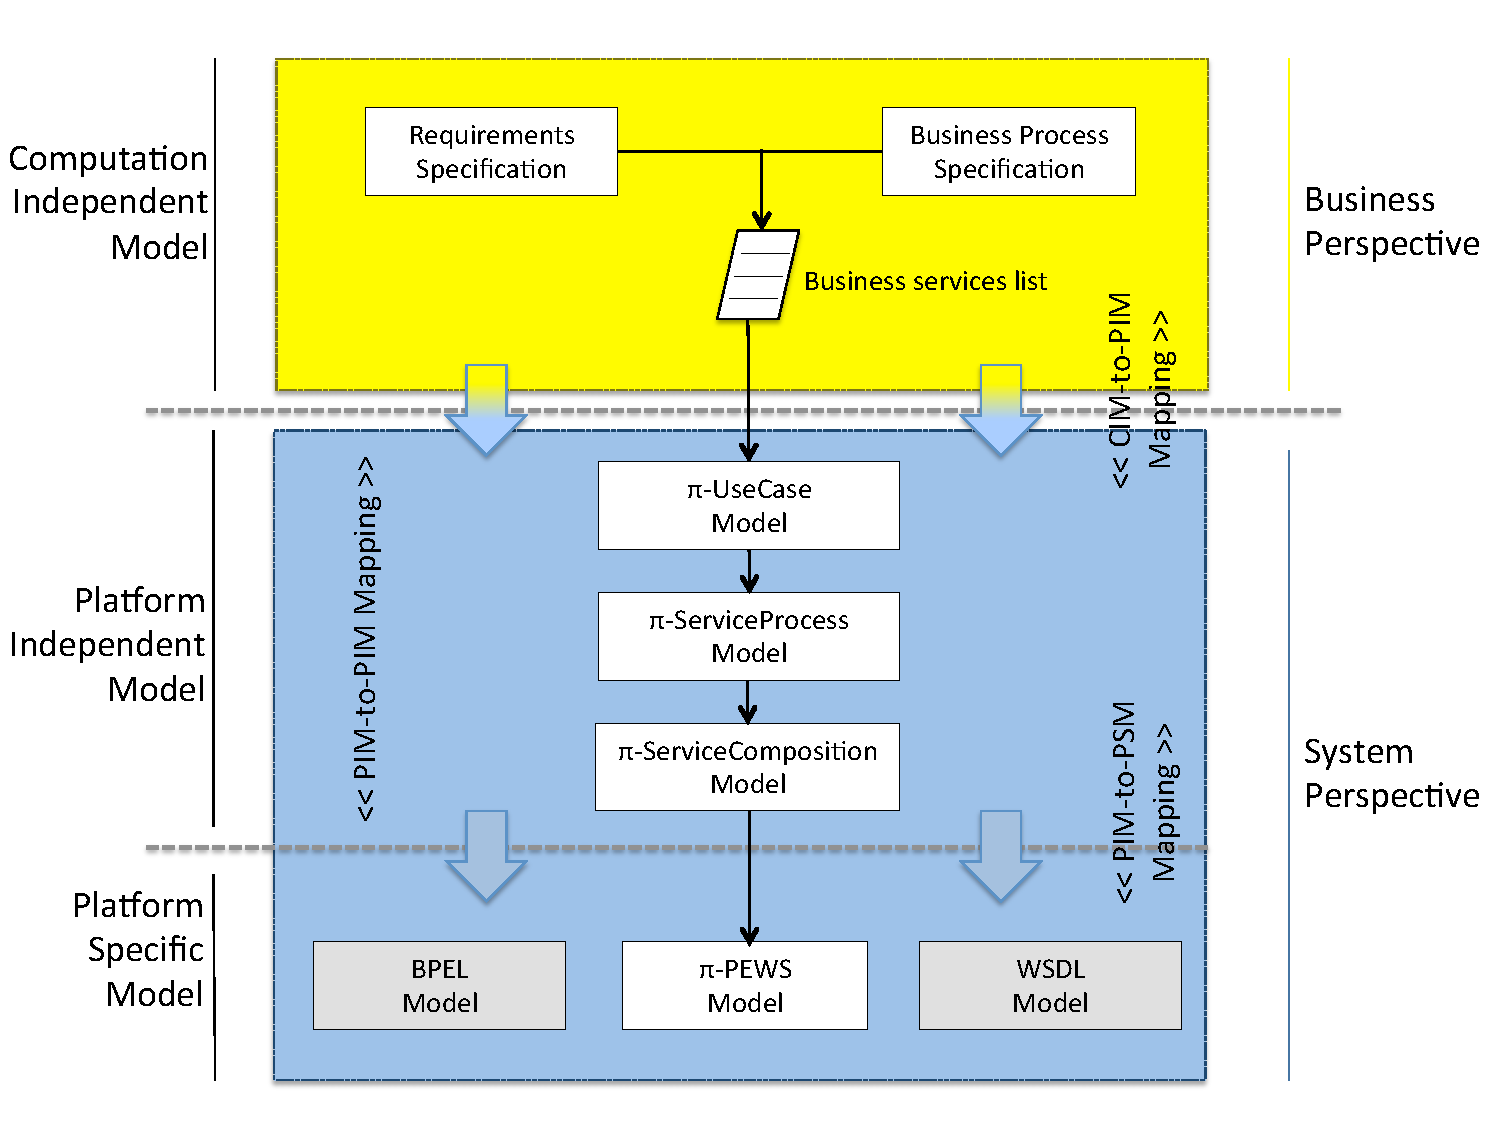
\includegraphics[width=0.8\textwidth]{chapters/methodology/figs/PiSOD-MProcess}
\caption{$\pi$SOD-M Development Process and Models.}
\label{fig:developmentProcess}
\end{figure}


 Computation Independent Models (CIM) aim to represent the business view, while
 Platform Independent Models (PIM) and Platform Specific Models (PSM) aim
 to represent the information system view and detail the information system to
 be implemented to fulfill the requirements of a business environment.

 Figure \ref{fig:developmentProcess} presents the $\pi$SOD-M development
 process, which defines a service oriented approach providing the guidelines for
 building service-based information systems (SIS), that was the result of the
 SOD-M extension described in figure \ref{fig:sodmExtensions}. 
 
%  Notice that it is
%  possible to have different platform models at the PSM level (figure
%  \ref{fig:sodmExtensions}), such as BPEL or WSDL. However,
%  $\pi$SOD-M defines the \textit{$\pi$-PEWS} model as platform specific model. We
%  choose \textit{$\pi$-PEWS} as platform  specific model because this language
%  can express in their specification, service compositions and restrictions on
%  services through contracts. Besides being a language developed by our research
%  group.

Next section presents the concepts that lead to modeling applications in
$\pi$SOD-M. These concepts form the basis of our methodology for modeling the
reliable service-based applications. 

\subsection{Methodology Concepts} 
\label{sec:concepts}

% $\pi$SOD-M proposes a new approach for defining non-functional
% aspects in service-oriented development. 

The concepts presented in figure \ref{fig:pisodm-concepts} represent the main
elements of the methodology used for system application modeling. The $\pi$SOD-M's
meta-model\footnote{\textit{Meta-model} is the construction of a collection of
``concepts'' (things, terms, etc.) within a certain domain. A model is an
abstraction of phenomena in the real world; a meta-model is yet another abstraction, highlighting properties of the model
itself. A model conforms to its meta-model in the way that a computer program
conforms to the grammar of the programming language in which it is written.}
concepts are used in all methodology meta-models. They
describe the key concepts that must be modelled in a service-oriented
application. The $\pi$SOD-M meta-model consists of the set of concepts for
modelling and development applications that use MDA. These concepts represent the reliable
service-based system development, and are present in the modelling any
application.


Notice that the three $\pi$SOD-M methodology views (\textit{Business, System}
and \textit{Policy}) are different to those levels proposed by the traditional
MDA literature: \textit{CIM, PIM} and \textit{PSM}. In the $\pi$SOD-M
meta-model, at different MDA levels, there are elements from the $\pi$SOD-M
concepts.  

\begin{figure}[ht!]
\centering
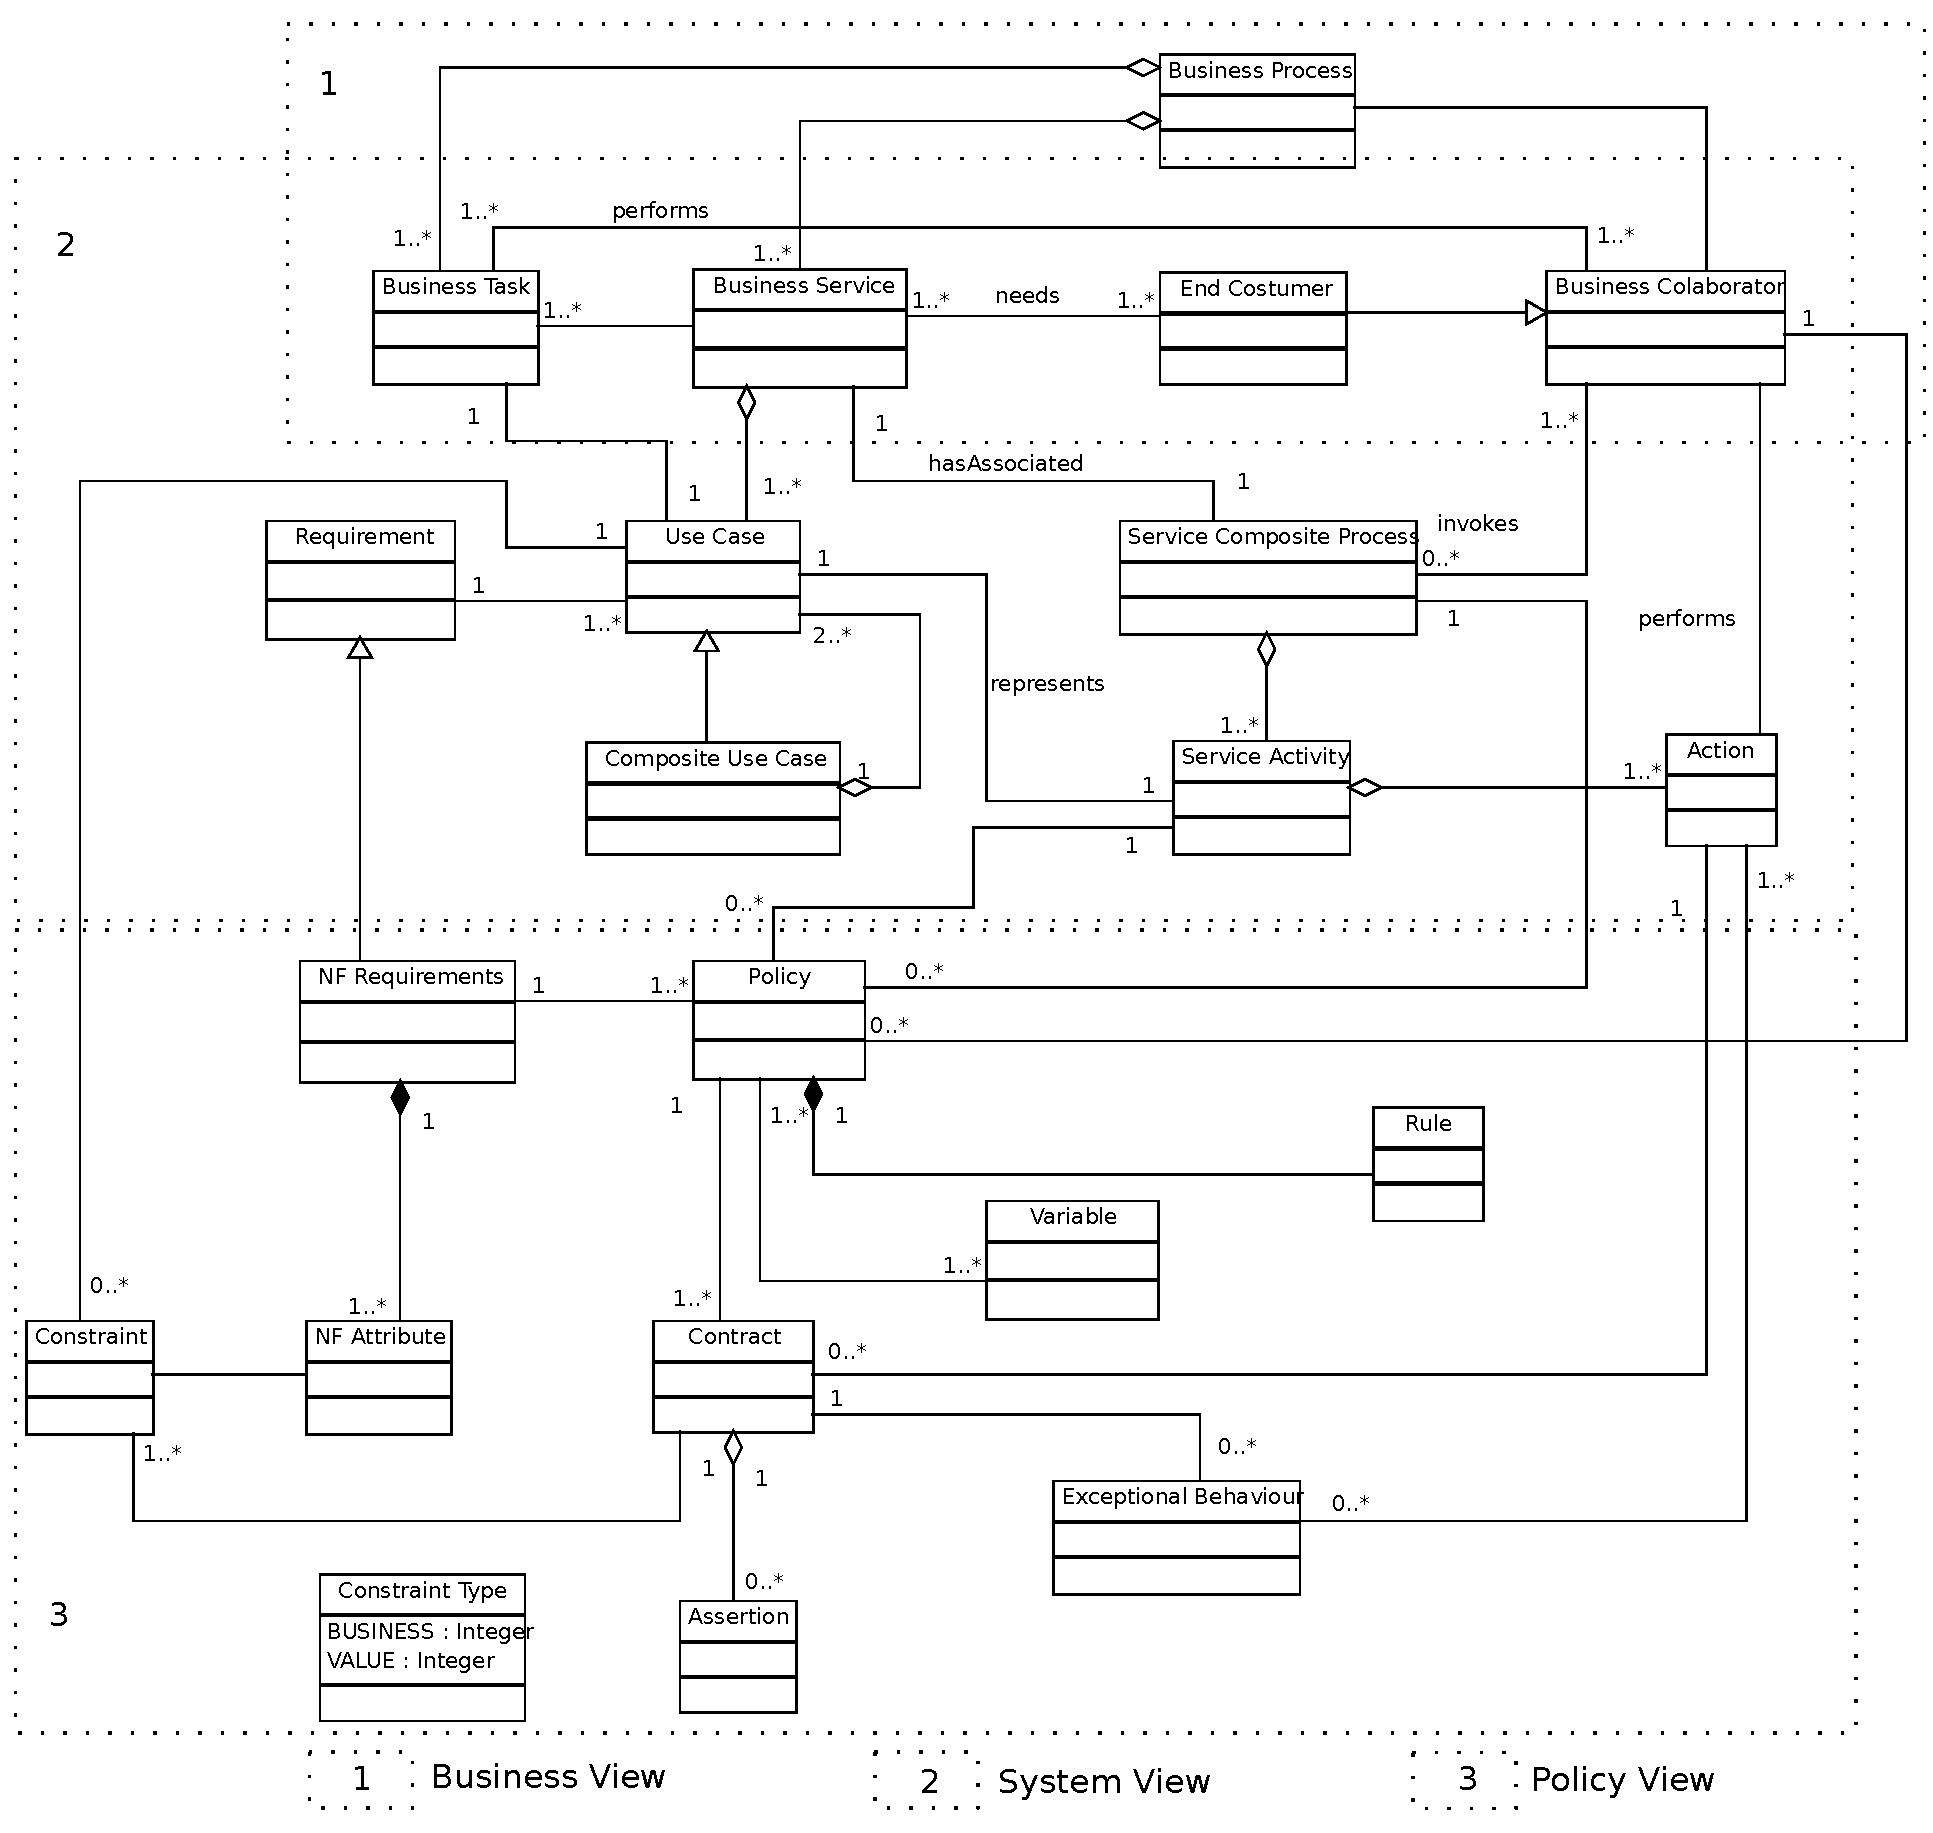
\includegraphics[width=.99\textwidth]{chapters/methodology/figs/PiSOD-M.pdf}
\caption{$\pi$SOD-M Concepts.}
\label{fig:pisodm-concepts}
\end{figure}
 
 All the proposed concepts and models for business modeling (CIM
 level), and for information system and policy modeling at PIM and PSM
 levels comprise the backbone for the $\pi$SOD-M based applications design.
 These concepts are important to identify the system requirements and properties throughout the
 development. Thus, the purpose of this section is to present a description of
 each concept, so that when applied and used, it can be seen in their
 proper modeling context. 
 


The methodology relies on a
set of concepts (represented as a meta-model) for modeling
reliable applications. These concepts are structured in three views:
\textit{Business, System} and \textit{Policy views} (figure
\ref{fig:pisodm-concepts}):

\begin{itemize}
  \item \textbf{Business view:} focuses on the business features
  that are the basis of an information system.  The concepts that
correspond to the \textit{Business View} describe business elements. There are
some concepts which correspond to both views (\textit{Business and System
Views}) and will be analyzed from both perspectives. 

  \item \textbf{System View:} focuses on the main features and
  processes for the information system development. The \textit{System View}
  concepts are used to describe the functionality and processing system. 

	\item \textbf{Policy View:} focuses on non-functional requirements and
	business constraints of the information system. The concepts that correspond to
	the \textit{Policy View} describe the NFRs and constraints related to the
	system functionalities. $\pi$SOD-M's main goal is to model non-functional
	requirements considering the models proposed by the SOD-M methodology.
\end{itemize}

% Figure \ref{fig:pisodm-concepts} shows a diagram that includes the
% set of concepts proposed by $\pi$SOD-M (which are organized in defined views),
% as well as the relationship between these concepts.

%  The SOD-M concepts do not provide this
% level of modeling. Thus, our proposal add non-functional
% concepts for modeling reliable software from early stages
% of service development (specification).

\newText{
The organization into different levels of abstraction of non-functional properties proposed by $\pi$-SOD-M relies on its concept of non-functional Requirement (NFR) defined  as a group of semantically correlated non-functional
attributes (NFA). For example, \textit{security} is an NFR that
comprises attributes such as \textit{confidentiality} and \textit{integrity}.
NFR are used for modeling global constraints, NFAs model non-fuctional characteristics that can be precisely measured, such as
 \textit{performance} \cite{RosaC04}. This kind of characteristics are closer to
 implementation. Then, the concept non-functional property proposed by
 \cite{RosaC04,Chung2009,MylopoulosBook99} is used for modeling  different
 types of software constraints. Thus, it generalizes the concepts NFR and NFA of
 our methodology. In $\pi$SOD-M, NFR and NFA are  modelled along the different
 modeling levels  as \textsc{constraint types} that can be grouped and 
 transformed into \textsc{contract types}, that can be transformed into
 \textsc{policy types}. A constraint type is used for representing  a
 non-functional property. }


 The $\pi$SOD-M concepts\footnote{The concepts marked with $^\ast$ are also part of
 the  \textbf{System view}} are:
 
\begin{itemize}
   \item \textbf{Business view:}
		\begin{itemize}
		  \item \textsc{Business process -} Represents the aggregation of
		  logically related tasks that are carried out to achieve a given business result.
		  \item \textsc{End consumer$^\ast$ -} Represents an entity that needs and
		  consumes business services. End consumers are those who pay (either with money or using
		  any other kind of value) to obtain a service that they use
		  themselves.
		  \item \textsc{Business service$^\ast$ -} Represents a result of a
		  business process (or part of it) providing value for an end consumer.
		  \item \texttt{Business task$^\ast$ -} Represents a business function
		  performed by a business collaborator as a part of a business process.
		  \item \textsc{Business collaborator$^\ast$ -} Represents an entity that
		  collaborates in the business processes of an organization, performing certain tasks needed
		  to provide a business service.
		  
		\end{itemize}

\item \textbf{System view:}	
	\begin{itemize}
	  \item \textsc{Requirement -} Represents a super type for functional and
	  non-functional requirements. Thus, the use cases can be related to both types
	  of requirements.	
	  \item \textsc{Use case -} Represents a set of actions performed by the system
	  to carry out part of a business service.
	  \item \textsc{Composite use case -} Represents a set of actions performed by
	  the system to carry out part of a business service, which can be broken down
	  into different use cases, which may in turn be basic or composite.
	  \item \textsc{Service composite process -} Represents a set of logically
	  related activities necessary for carrying out a business service.
	  \item \textsc{Service activity -} Represents a behaviour (set of individual
	  actions) forming part of the execution flow of a business service.
	  \item \textsc{Action -} Represents a fundamental behaviour unit that is part
	  of a service activity and describes some transformation or processing in the
	  system being modelled.
	\end{itemize}
	
\item \textbf{Policy view:}		
	\begin{itemize}
		  \item \textsc{Non-Functional (NF) Attribute -} An attribute that describes
		the quality or characteristics of a functional requirement. For example
		\textit{confidentiality} and \textit{privacy} is an example for a non-functional
		attribute for the functional requirement \textit{user registration}.
		  \item \textsc{Non-Functional (NF) Requirement -} A group of semantically
		correlated non-functional attributes (NFA). For example, \textit{security} is
		an NF Requirement that comprises attributes such as \textit{confidentiality}
		and \textit{integrity}.
		  \item \textsc{Constraint -} A constraint prevents the system
		  from achieving more than its goal. With the definition of constraints, the
		  system  can be more robust, and unexpected problems can be solved before they
		  happen. For example, in a banking system, the customer can only withdraw
		  money if they have a positive balance in the account.
		    \item \textsc{Constraint Type -} Represents the types of constraints, that
		    may be on a system function or values. This entity can have their
		    property setted as a business and data (value) constraint (expressed as an
		    attribute). 
		  \item \textsc{Contract -} Is the formalization of obligations (requires) and
		  benefits (ensures) of a function, service activity or component.
		  The following questions can be used to define contracts: \textit{What does it
		  expect? What does it guarantee?} Contracts are crucial to software correctness
		  and therefore they should be part of the design process. An interface is a
		  kind of contract.
		  \item \textsc{Assertion -} Represents a predicate or a state of the
		  application before it runs (its preconditions), or the state when it is
		  finished running (post-conditions);
		  \item \textsc{Exceptional Behaviour -} Are alternative execution paths if
		  any condition or restriction is not respected. For example, if a user's
		  password is not correct after three attempts, the user account is locked for
		  security reasons.
		  \item \textsc{Policy -} A policy is a set of rules applied to a particular
		  scope. This scope can be defined as an action, an activity, a function or a
		  workflow. A policy is a composition of contracts applied to a non-functional
		  application requirement. For example, a security policy of a system constraint
		  may include authentication, access and data privacy properties.

		  \item \textsc{Rule -} Represents information about an event, condition, and
		  action where the event part represents the moment in which a constraint can be
		  evaluated according to a condition represented by the condition part and the
		  action to be executed for reinforcing it represented by the action part.
		  \item \textsc{Variable -} Represents a symbolic name given to some known
		  information. A variable are related with a Policy. A Policy can have one or
		  many variables. Each Variable has a name and a type.
	\end{itemize}
\end{itemize}





% 
% For example, in the \textit{$\pi$-UseCase} model (\textit{PIM} level) uses the
% {\sc Use Case\footnote{We use {\sc capitals} for referring to meta-models' classes.}},
% {\sc Constraint, Business Service, End Costumer} and {\sc NF Requirements}
% concepts to represent what is being modeled. {\sc Business Service} and
% {\sc End Costumer} are elements that model \textit{Business} concepts, while
% {\sc Use Case} models \textit{System} concepts and, {\sc Constraint} and {\sc
% NF Requirement} model \textit{Policy} concepts. The same is true for all other
% $\pi$SOD-M models, \textit{$\pi$- ServiceProcess,
% $\pi$-ServiceComposition} and \textit{$\pi$-PEWS}. The relationships
% among these $\pi$SOD-M concepts are also presented in figure
% \ref{fig:pisodm-concepts}, and especially the {\sc Policy} level for quality
% requirements modeling.
% 
% \bigskip
% \bigskip
% 
% Considering the set of concepts presented, each of them aims model
% important parts of the application. The services-based systems represent
% business relationships through {\sc Business Services},  in a more abstract
% level. {\sc Business Services} make up different application services, in order
% to perform a business relationship. Services are system features being
% modeled by {\sc Use Cases}. {\sc Use Cases} are refined at each
% development iteration, where s set of restrictions are
% specified for each function or service. System restrictions are represented
% through {\sc Constraints}, {\sc Contracts} or {\sc Policies}. {\sc Constraints}
% are restrictions on {\sc  Use Cases}, while {\sc Contracts} are restrictions on
% {\sc Actions}, or their specific functions, and {\sc Policy} is a restriction
% on a group of services that can be represented as {\sc Service Activity} or a
% {\sc Service Composite Process} . Thus, these terms specify particulars of the
% application at different modeling levels.
% 
% 
% Based on this, so that all the system features needed are specified, these
% concepts relate to each other in order to describe each use case, function,
% service or  application process. One {\sc Requirement}, whether functional or
% non-functional, represents by one or more {\sc Use Cases}. For example, a
% payment process can be modelled through the use cases that represent withdrawal
% and deposit of money in transaction of customer accounts. A payment process also
% requires the guarantee of a complete transaction and data security. Thus, some
% use cases can compose a single requirement.
% 
% A {\sc Composite Use Case} represents a type of {\sc Use Case}. This type of
% use case abstracts a more macro function, and may contain extra functions to be
% performed so that the process is complete. For example, to publish a song in a
% social network, you must choose which song you want to publish, authenticate, so
% that the music you're listening is published. We consider this type of use case,
% a use case compound.
% 
% Each {\sc Use Case} has many {\sc Constraints} (business or
% value constraints). Business constraints represents restrictions expressed on
% functions and how they may be implemented. Value constraints are restrictions on the
% service interface, which detail the desired values  for input and output
% data. Each constraint is associated with {\sc Non-Functional Attributes} (NFA).
% 
% A {\sc Contract} consists of a set of {\sc Constraints}. As a {\sc Contract}
% represents a composition of assertions, each {\sc Constraint} are
% refined into {\sc Assertion} that will compose one {\sc Contract}. For
% example, a contract for the payment operation by credit card, the value should
% not be less than 10 euros and the user should always receive a purchase
% confirmation by email or by phone message. This set of restrictions will be
% composed into a single contract for payment transactions. These constrains are
% also associated with non-functional attributes, e.g., \textit{reliability,
% transactions and privacy data}.
% 
% An {\sc Exceptional Behavior} represents a non excepted system behavior or
% a contract violation. When this happens other function is called
% or the application process is stopped. In $\pi$SOD-M, this entity represents the
% contract violation. For example, if the bank does not authorize the payment, the
% system or service offers alternative forms of payment such as a bank invoice or
% purchase via PayPal.
% 
% 
% Finally a {\sc Policy} groups similar {\sc Contracts}, \textit{e.g.}
% contracts for the application safety, or contracts on the system performance are
% grouped as policies. For example, payment and authentication contracts are
% grouped into \textit{security} policy, as well as contracts that require a
% time-out processing, are grouped into \textit{performance} policy. Each policy
% is associated with a non-functional requirement, a set of {\sc Rules} and
% {\sc Variables}. Each {\sc Non-Functional Requirement} is associated with
% one or more {\sc Non-Functional Attributes}.

 The following next sections will describe the example scenario to better
 explain the $\pi$SOD-M meta-model and the methodology concepts.


\subsection{Case Study}
\label{sec:example}

We use a case study in order to better describe specific details of the
methodology proposed in this work. 

% We will specify the
% application of concepts and models in this case study so that each detail of the
% methodology is covered. We cover all $\pi$SOD-M features through examples at
% the same time in which the application is being developed, the concepts,
% activities and models of our methodology are explained.

Consider the following scenario: An organization
wants to provide the service-based application ``\textit{To
Publish Music}'' that monitors the music a person is listening
during some periods of time and sends the song title to this
person's Twitter or Facebook accounts. More specifically, this social
network user will have their status synchronized in both Twitter\footnote{Twitter is an online social networking service and micro-blogging service that enables its
users to send and read text-based posts of up to 140 characters, known as
``\textit{tweets}''.} and Facebook\footnote{Facebook is a social networking
service and website. Users may join common-interest user groups, organized by
workplace, school or college, or other characteristics, and categorize their
friends into lists}, with the title of the music the user is listening
in Spotify\footnote{Spotify is a music streaming service offering digitally
restricted streaming of selected music from a range of major and independent
record labels. Spotify allows registered users to integrate their account with
existing Facebook and Twitter accounts.}. The user may
also want to download music. For this, the user needs to process the purchase of music
they want to download. Payments will be processed via PayPal or credit card. All services
are available via Spotify and our application needs to interact with Spotify
users, so they can listen music, publish on Facebook and Twitter, and
purchase music online.  The corresponding use case model is illustrated in in
figure \ref{fig:example_usecase}.

% Lets consider the use case model illustrated in figure
% \ref{fig:example_usecase}.
%  Figure \ref{fig:example_usecase} shows the use case model for the ``\textit{To
% Publish Music}'' application. 


\begin{figure}[ht!]
\centering
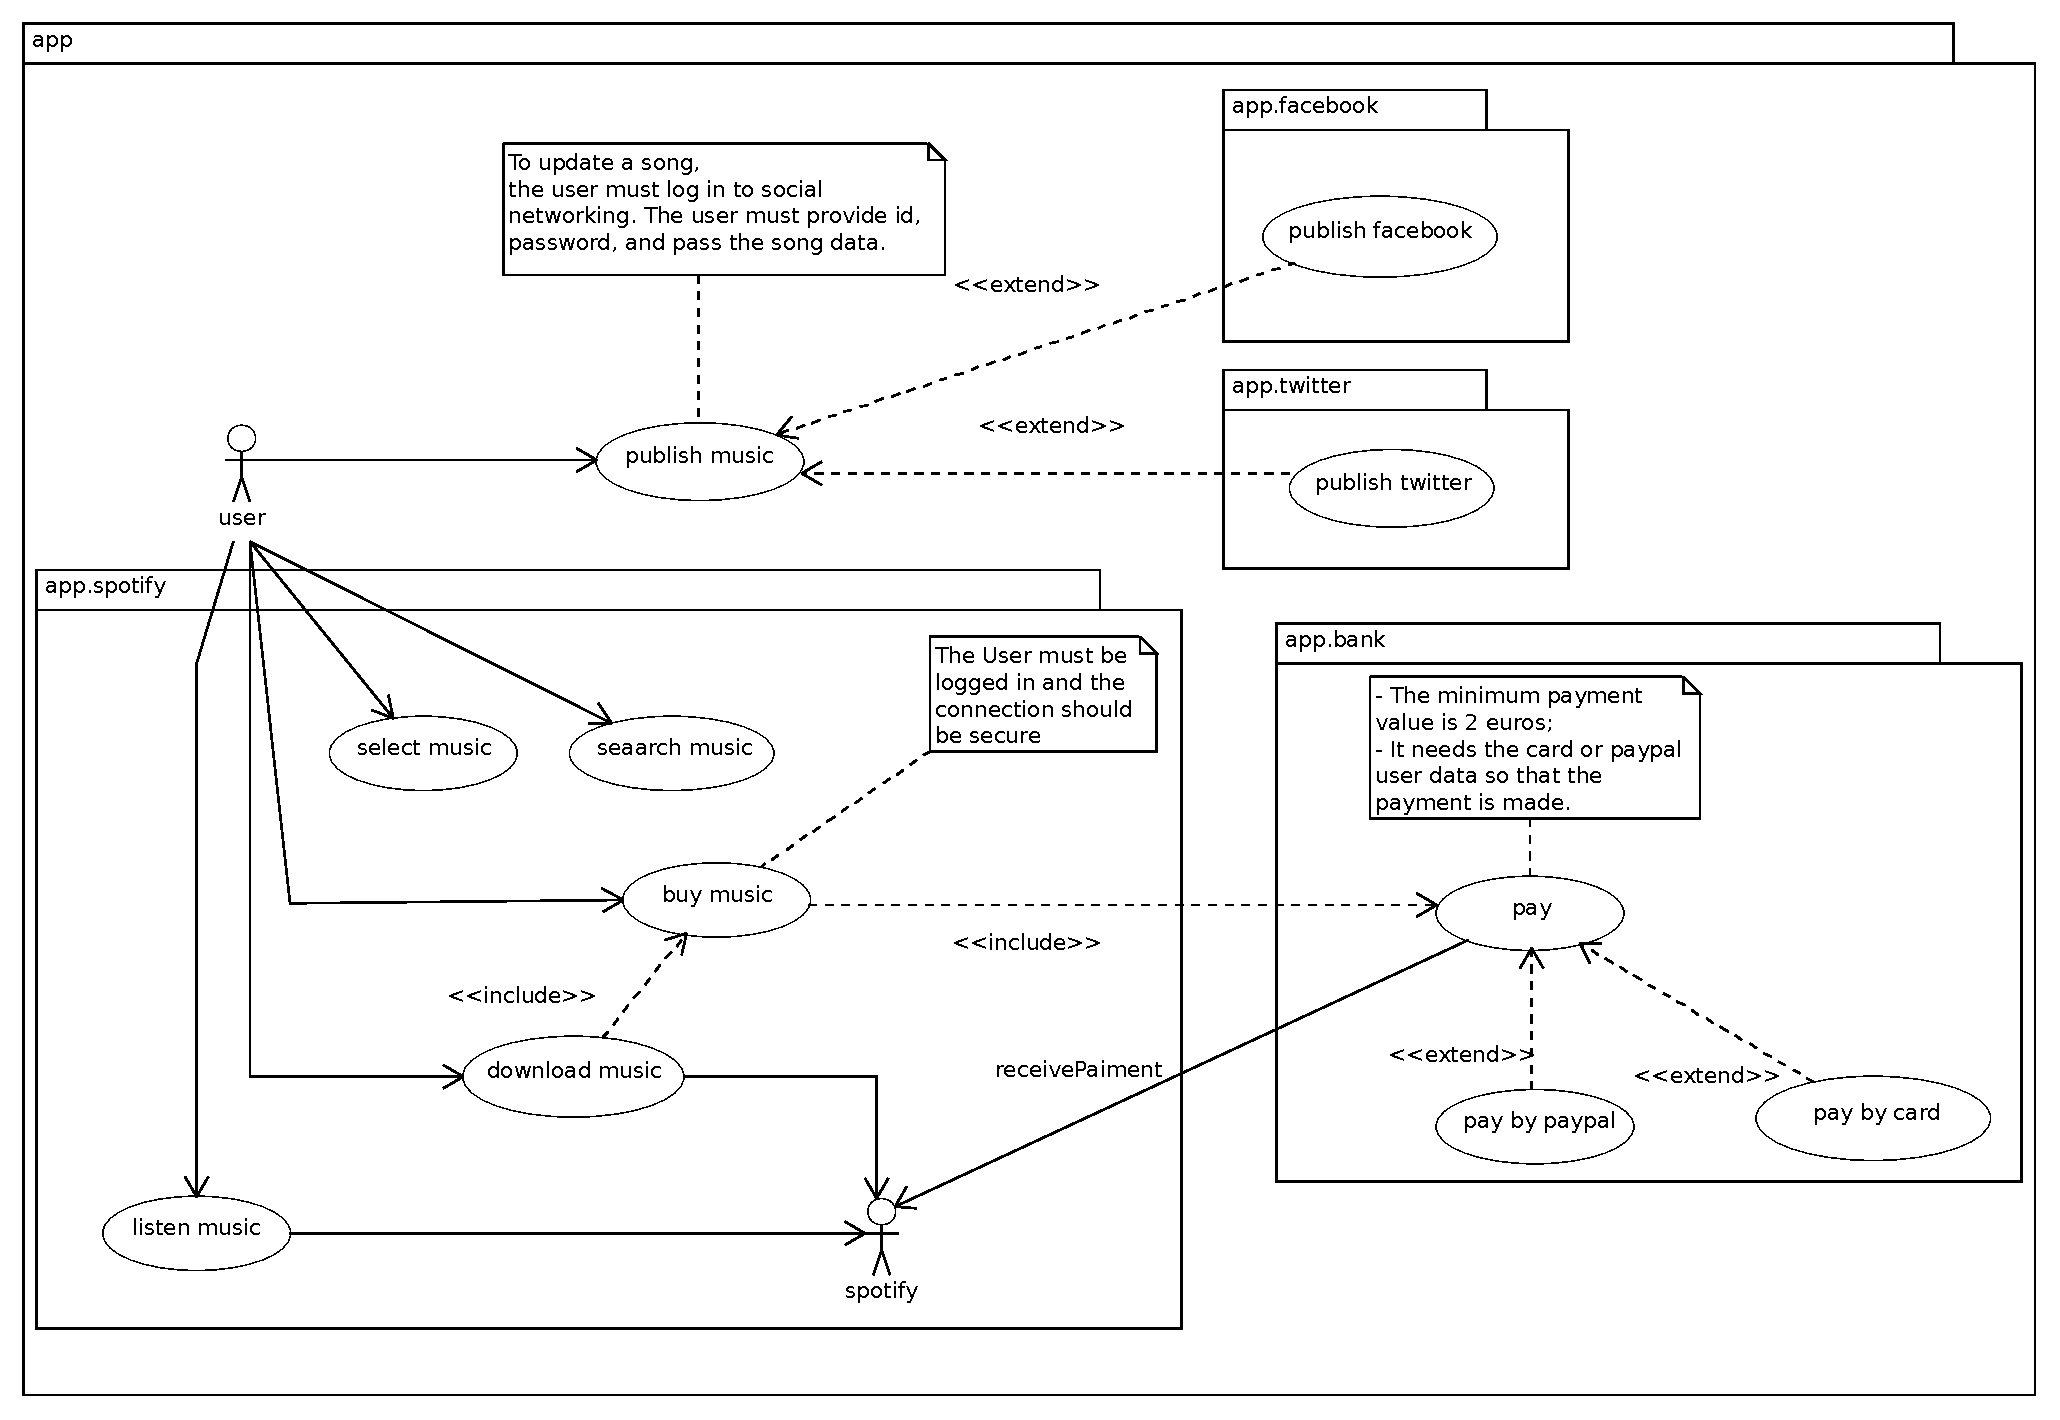
\includegraphics[width=.95\textwidth]{chapters/methodology/figs/runningExampleUCSingle.pdf}
\caption{Use Case Model ``\textit{To Publish Music}'' - Spotify Music Service.}
\label{fig:example_usecase}
\end{figure}



% As long as the user listens the music, they can
% publish the music information on social networks. For downloading music, it is
% necessary to purchase the song the user wants. To publish songs, the user must 
% login and authenticate on the social networks services, and for that there are
% constraints to be modelled and implemented. The same is true for purchasing
% music, where some integrity checks and confidentiality of the credit card
% data are required.


Figure \ref{fig:example_serviceprocess} shows the activity model for our
scenario. It starts by contacting the music service Spotify for retrieving the
user's musical status.  If the user wishes to download a particular song, they
can download the song to purchase (activities \textit{Buy Music} and
\textit{Download Music}). Finally the user can publish the music. The activity
\textit{publish music} can also be modelled as a parallel workflow for updating
different social networks, as follows: Twitter and Facebook services can be
contacted in parallel for updating the user's status with the corresponding song title.

\begin{figure}
\centering
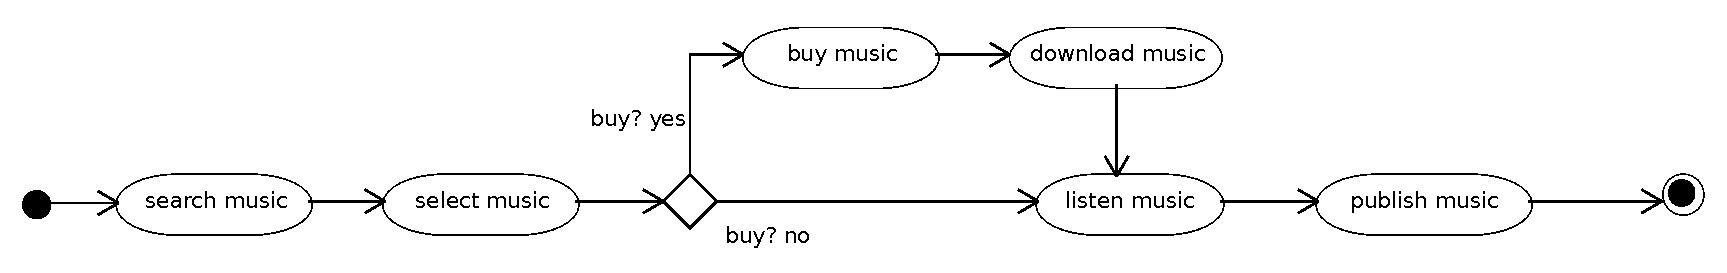
\includegraphics[width=.95\textwidth]{chapters/methodology/figs/runningExampleSPSingle.pdf}
\caption{Service Process Model ``\textit{To Publish Music}''.}
\label{fig:example_serviceprocess}
\end{figure}

The execution flow is described as follows. Each action from the activity
diagram represents one or more functions in the application. Each function or
service has an interface, consisting of its input and output, and the
specification of how to call this function/service. An activity must
be executed according to the rules identified in the use case model. For example, the
``\textit{publish music}'' action (figure \ref{fig:example_serviceprocess}),
can be refined into two flows: (i) a flow to publish on Twitter and (ii) another to
update the Facebook, since each service has different rules for update and
login.

Given a set of services with their exported methods (known
in advance or provided by a service provider), building service-based
applications is a task that implies expressing an application logic as a service
composition together with some restrictions. 



\begin{figure}[ht!] 
\centering
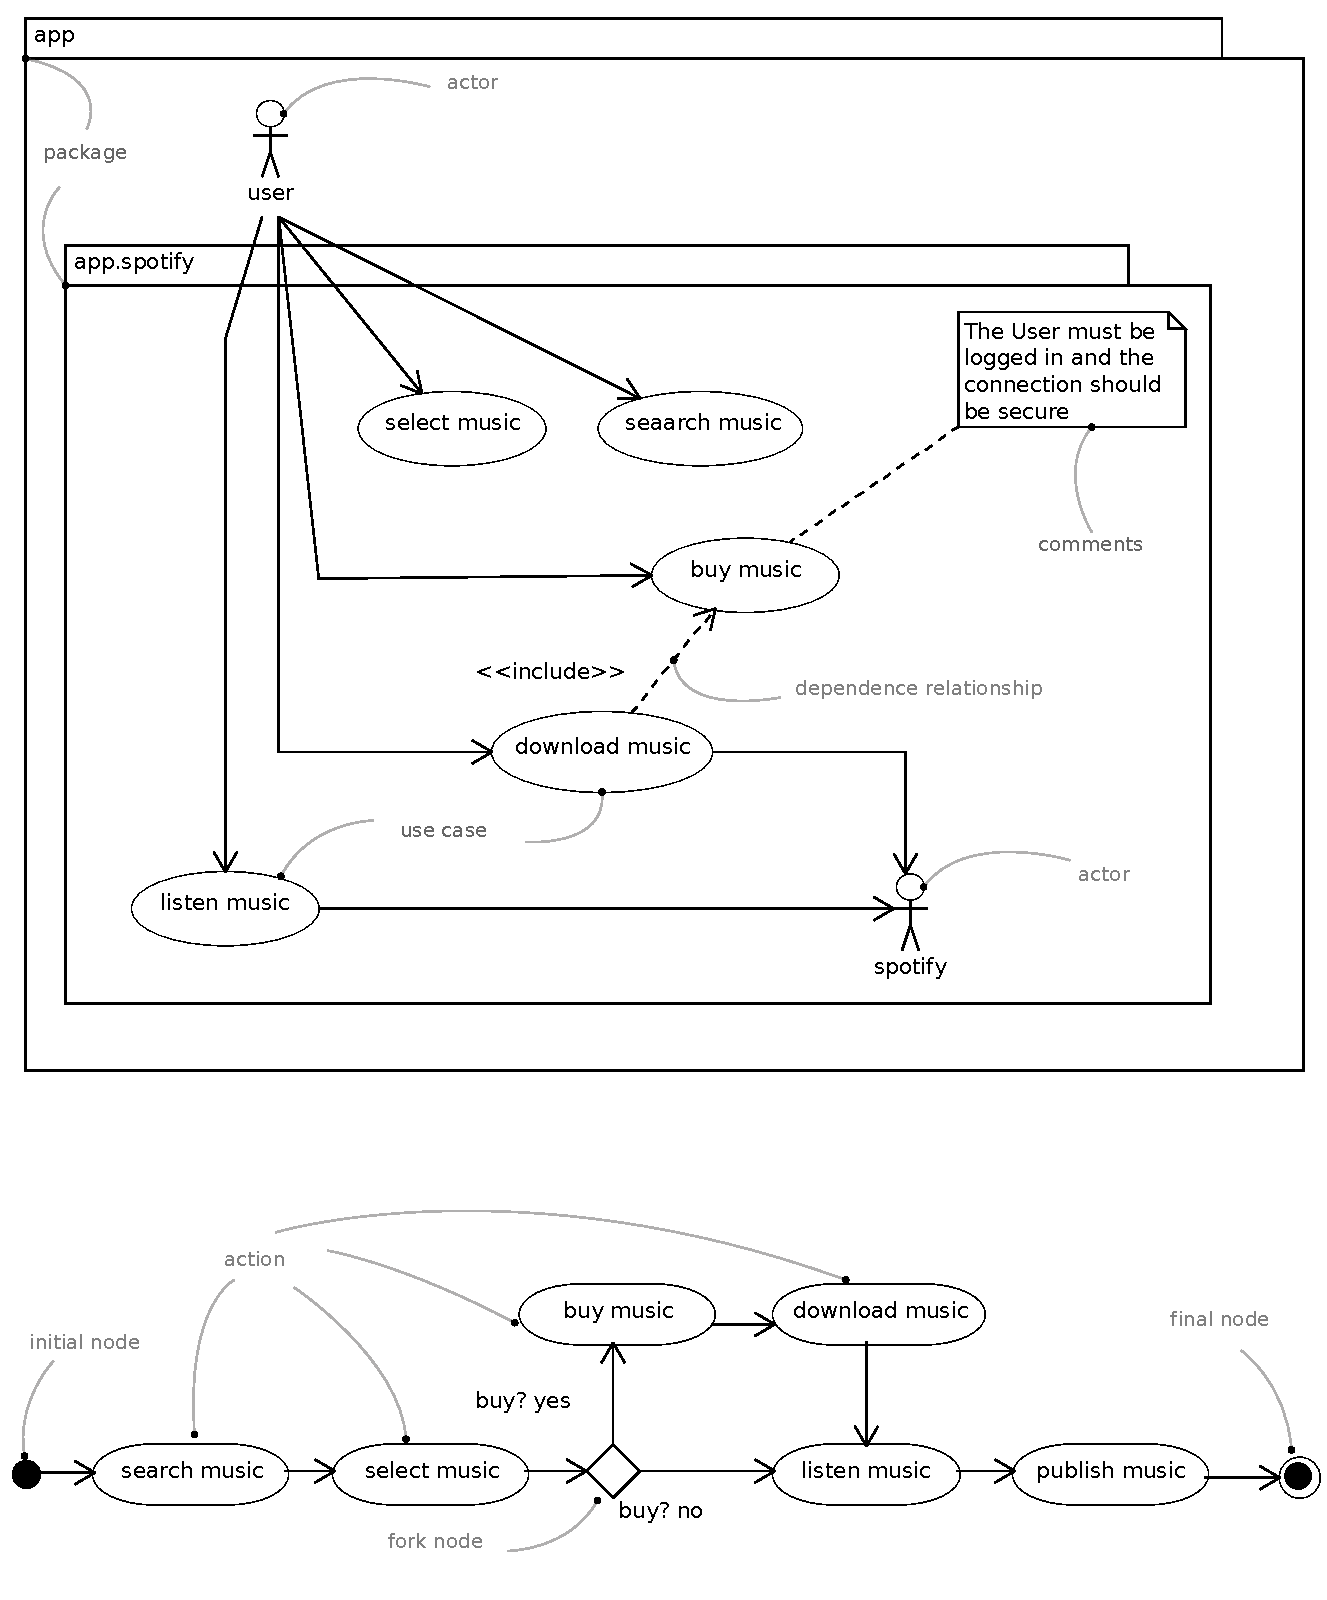
\includegraphics[width=.95\textwidth]{chapters/methodology/figs/runningExampleUCSingle_detail.pdf}
\caption{Traditional UML Concepts.}
\label{fig:umlConcepts} 
\end{figure}

Both models presented in figures \ref{fig:example_usecase} and \ref{fig:example_serviceprocess} use the
 traditional UML to design requirements in use case diagram and workflow actions
in the activity diagram. Figure \ref{fig:umlConcepts} presents
some of the main UML concepts that are used to model system diagrams. The
structure of each $\pi$SOD-M model will be detailed in accordance with their
respective meta-model and transformations necessary for achieving the aim of modeling
reliable applications.  
 
% This example scenario will be used to exemplify the
% concepts of the $\pi$SOD-M methodology as well as to model the system properties from the
% use case to service composition model.  

\section{Platform Independent Models}
\label{sec:pim-pisodm}


The \textit{Platform Independent Models (PIM)} are used for modeling the
system functionality, abstracting technological details. 

% These models can be used on different deployment platforms. Since $\pi$SOD-M
% defines a method for developing service-oriented applications, such models focus on identifying the services to be
% offered by the system, as well as on identifying general functionalities,
% processes and constraints.

The models proposed at $\pi$SOD-M's PIM level are (figure
\ref{fig:developmentProcess}): \textit{ $\pi$-UseCase, $\pi$-ServiceProcess} and \textit{
$\pi$-ServiceComposition}. They provide concepts for expressing the design of:
(\textit{i}) system requirements and constraints; (\textit{ii}) external
services and their compositions; (\textit{iii}) execution flow; (\textit{iv})
input and output service restrictions; (\textit{v}) service contracts and
actions; and (\textit{vi}) policies for the implementation of business services.
We use these models to provide a representation of the system and to
specify its restrictions. 

%Each of the three Platform Independent Models are presented next.


\subsection{\textit{$\pi$-UseCase} Model}


The \textit{$\pi$-UseCase} (figure \ref{fig:usecasemodel}) is used
to describe the functionalities (services and other functionalities) of the system. The
services are represented in this model as use cases. We design this model by
using the UML use cases, with a small extension for considering constraints.
Application constraints are represented by stereotyped use cases and comments
related to them. Each constraint describes what will be checked for a
particular application function be executed. Figure \ref{fig:piUseCaseExample}
shows\footnote{The annotation in this figure are not part of
the model. They are included for didactic explanation only. The same applies for
the other figures in this section which present the same type of annotation.} an
example of how to describe constraints on use cases in $\pi$SOD-M. We use part
of our case study to present them. Each use case may have multiple constraints.
In this example the \textit{publish music} use case has an authentication
constraint (\textit{user must authenticate}). For a song to be published on any
social network it is necessary to provide data privacy. The constraint type
concerns the authentication values and the constraint has an non-functional
attributes. The use case is also related with requirement, a business service
and a non-functional requirement properties.
 
% The main difference between the \textit{extended use case} diagram proposed by
% SOD-M\cite{valeriaThesis} and our \textit{$\pi$-UseCase} diagram is the
% inclusion of concepts that represent the modeling of non-functional requirements (\textit{policy view}). 


\begin{figure}[ht!] 
\centering
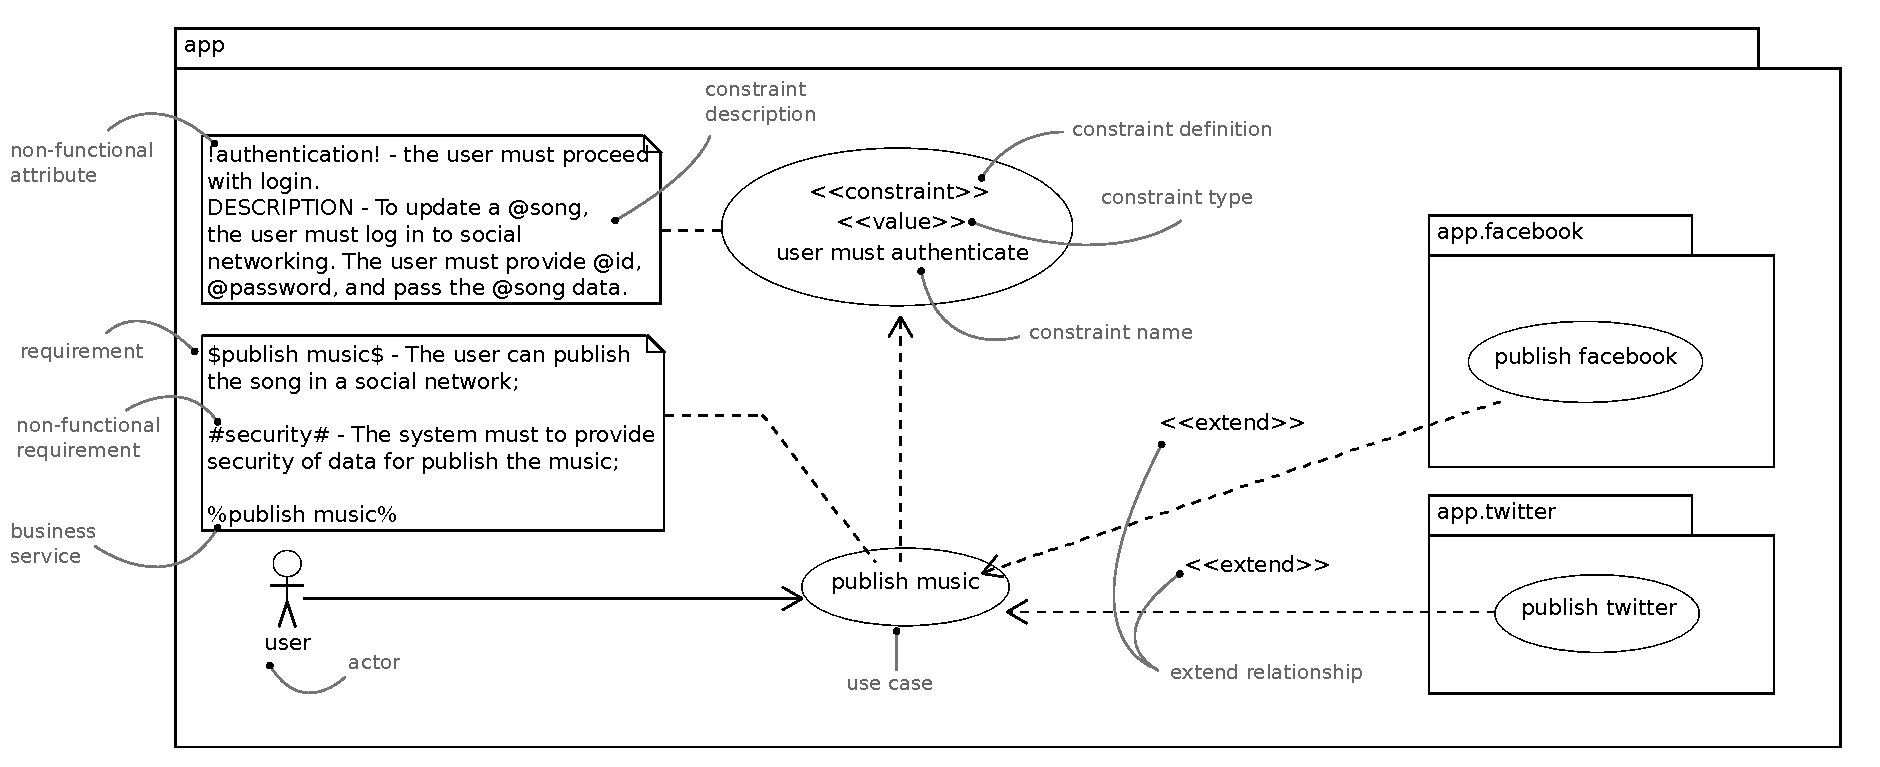
\includegraphics[width=.99\textwidth]{chapters/methodology/figs/piUseCase-Example_detail.pdf}
\caption{$\pi$-UseCase model Example.}
\label{fig:piUseCaseExample} 
\end{figure}

% This representation will be described in detail throughout this section, however
% the general \textit{$\pi$-UseCase} concepts are presented in figure
% \ref{fig:piUseCaseExample}. This representation shows only an overview of how
% to model system features and restrictions, and describe the concepts in this
% level of abstraction.
%  
 
 \subsubsection{\textit{$\pi$-UseCase} Diagram, Terms and Concepts} 
  

The \textit{$\pi$-UseCase} model describes the
functional aspects of the application being developed and the restrictions
that applies to each of them. These restrictions are modeled using the concepts:
(i) constraint type and (ii) non-functional requirement with its
specific attribute.


 A \textit{$\pi$-UseCase} model is a way to represent features of an
 application, services, constraints, and consumers of application functionality.
 
%   What differentiates
%  this model from others is its particular content and the form of their
%  presentation.
%   
%  This model is particularly essential for the organization and modeling of
%  application behavior. The behavior is represented by a normal and 
%  exceptional flows. In both cases there are restrictions that must be verified.
%  The restrictions may be on variables, values or function calls. 

 \begin{figure}[ht!] 
\centering
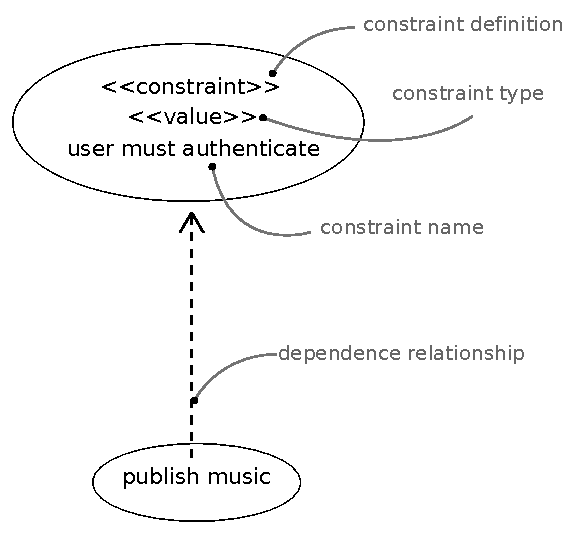
\includegraphics[width=.4\textwidth]{chapters/methodology/figs/constraints_detail.pdf}
\caption{Constraint Representation.}
\label{fig:constraint_detail} 
\end{figure}

 All constraints are described by stereotyped use cases. Every relationship
 between an use case and a constraint is done through a dependency relationship
 (from UML). All use cases that are related with constraint must be
 represented such as described in figure \ref{fig:constraint_detail}. A
 constraint is defined by a stereotype, containing its \textit{type} and
 \textit{name}. The {\sc Constraints} are represented by a stereotyped use case
(\textit{<<constraint>>}).

 \begin{figure}[ht!] 
\centering
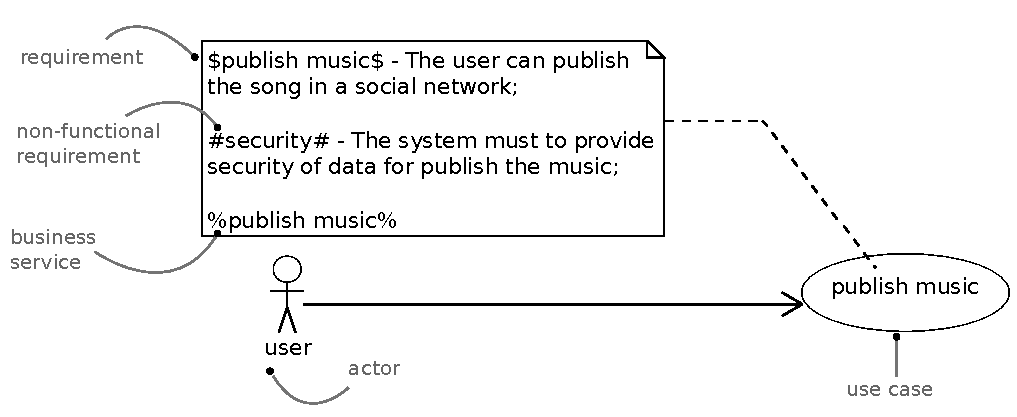
\includegraphics[width=.75\textwidth]{chapters/methodology/figs/nfr_detail.pdf}
\caption{Non-functional Requirement Representation.}
\label{fig:nfr_detail} 
\end{figure}

Each use case is related with one or more system requirements. Moreover, these
use cases are related to non-functional requirements necessary for the proper
execution of the application function. Similarly, the function described by an
case of use can be part of a business service (in the case of service remote
calls). These information to a specific use case may be described through
comments as described in figure \ref{fig:nfr_detail}. All these information
must be associated with the use case and its constraints.
 
 \begin{figure}[ht!] 
\centering
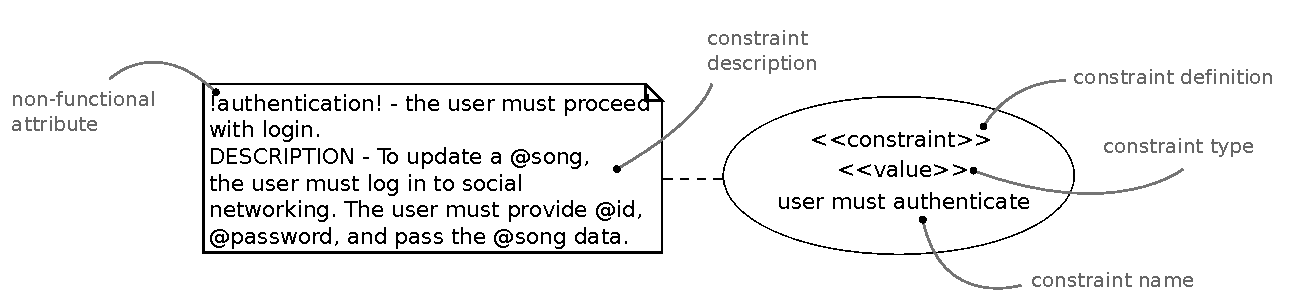
\includegraphics[width=.85\textwidth]{chapters/methodology/figs/nfa_detail.pdf}
\caption{Non-functional Attribute Representation.}
\label{fig:nfa_detail} 
\end{figure}

The constraints are always related to non-functional requirements. More
specifically, each constraint describes a non-functional attribute,
\textit{e.g.} \textit{authentication} (presented in figure
\ref{fig:nfa_detail}). A constraint consists of the constraint description and
the identification of variables be verified (by an \textit{@}, for example
\textit{@song}), the identification of the non-functional attribute and its
description. 

  

% Considering the $\pi$SOD-M concepts, the \textit{$\pi$-UseCase} model
% describes the representation of system functionalities to be modelled in this
% early stage of the design. The system features and its interactions are
% presented using meta-model entities.

These concepts that are described in the $\pi$SOD-M  meta-model and used in
\textit{$\pi$-UseCase} represent the concepts we identified necessary
for reliable service-based modeling. 

%  are presented in each abstraction level
% in order to better describe and refine properties of the applications that are
% being developed.
%  
%  \bigskip 
%  \textbf{Properties} 
%  \bigskip 
%  
 
 \subsubsection{Meta-model} 
 
 
The concepts modelled in the \textit{$\pi$-UseCase} meta-model are: {\sc
Business Service, End Consumer, Requirement, Use Case, Composite Use Case, Non-Functional Requirement,
Non-Functional Attribute} and {\sc Constraint}.  Figure
\ref{fig:usecasemodel} presents the \textit{$\pi$-UseCase} meta-model and the
relationship between each concept. We highlight the elements that represent the
\textit{policy view}. 
 
 
% The \textit{$\pi$-UseCase} elements aim to describe system properties and system
% functions in a abstract way, with a coarser granularity. Without considering any
% application details, they specify the general features of the system and its
% restrictions, as services or other functions. For example, i

In the \textit{$\pi$-UseCase} an {\sc End Consumer} is represented by an {\sc
Actor} (figure \ref{fig:usecasemodel}). An {\sc Actor} is related to {\sc Use Cases}
(from the original UML definition), while a {\sc Composite Use Case} is a set of
actions performed by the system which can be broken into different {\sc Use Cases}.


{\sc Business Service} aggregates several {\sc Use Cases} (figure
\ref{fig:usecasemodel}), simply put, a service can be expressed by one or more
use cases. Notice that not always an use case will be part of a business
service. However, using our approach, we can identify in the early stages of
modeling, which use cases are related to business services.


\begin{figure}[ht!]
\centering
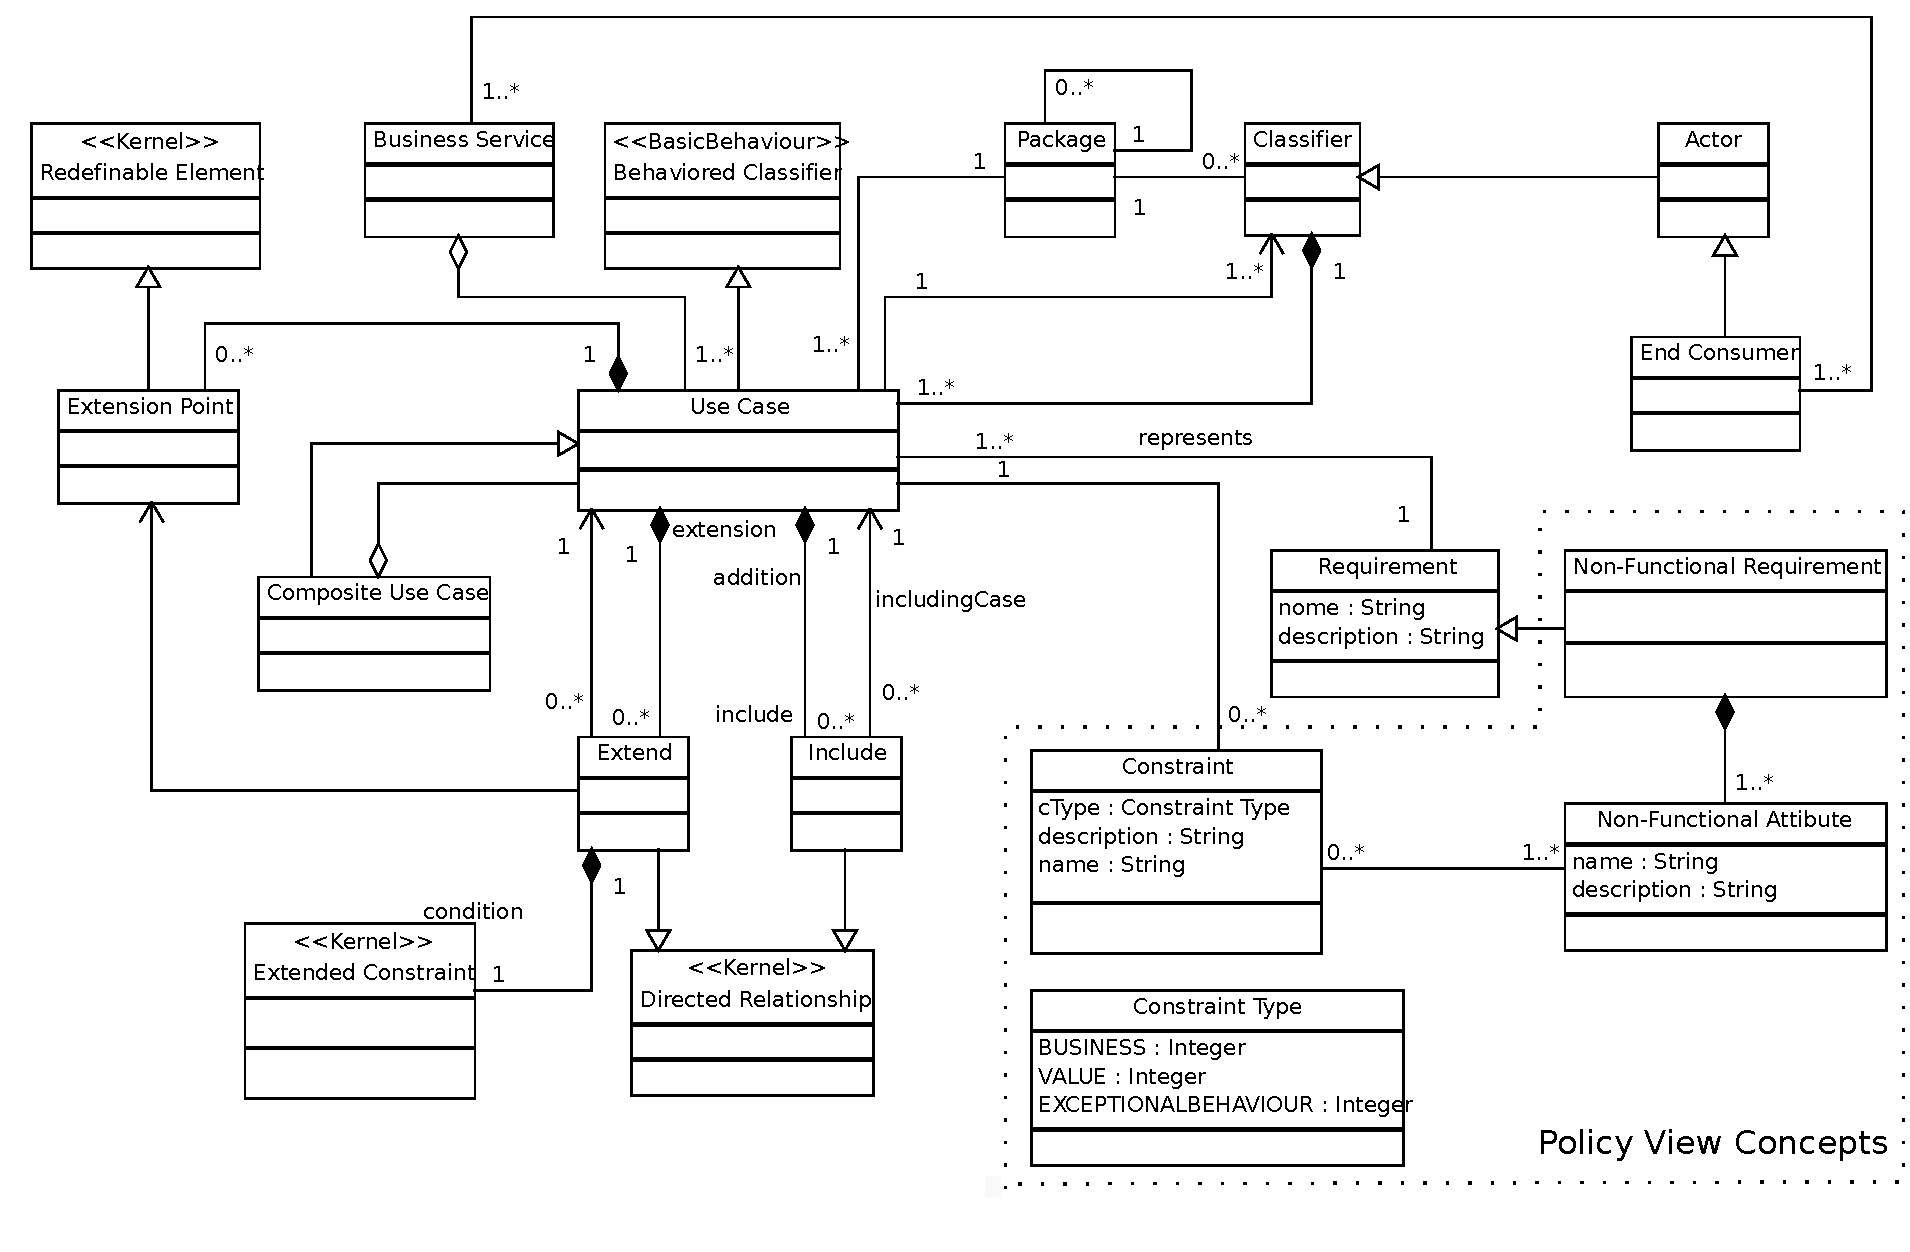
\includegraphics[width=1.0\textwidth]{chapters/methodology/figs/PiUseCaseMetamodel.pdf}
\caption{$\pi$-UseCase Concepts (Meta-model).}
\label{fig:usecasemodel}
\end{figure}


The {\sc Business Collaborators} concept are represented in the
\textit{$\pi$-UseCase} model through {\sc Packages}. A {\sc Business
Collaborator} represents an external service or a system that interact
with the application that are being modelled. Each {\sc Business Collaborators}
combines the features described in each {\sc Package}. Thus, the
services functions can be specified being grouped into packages (figure
\ref{fig:businessCollaborator}).

\begin{figure}[ht!]
\centering
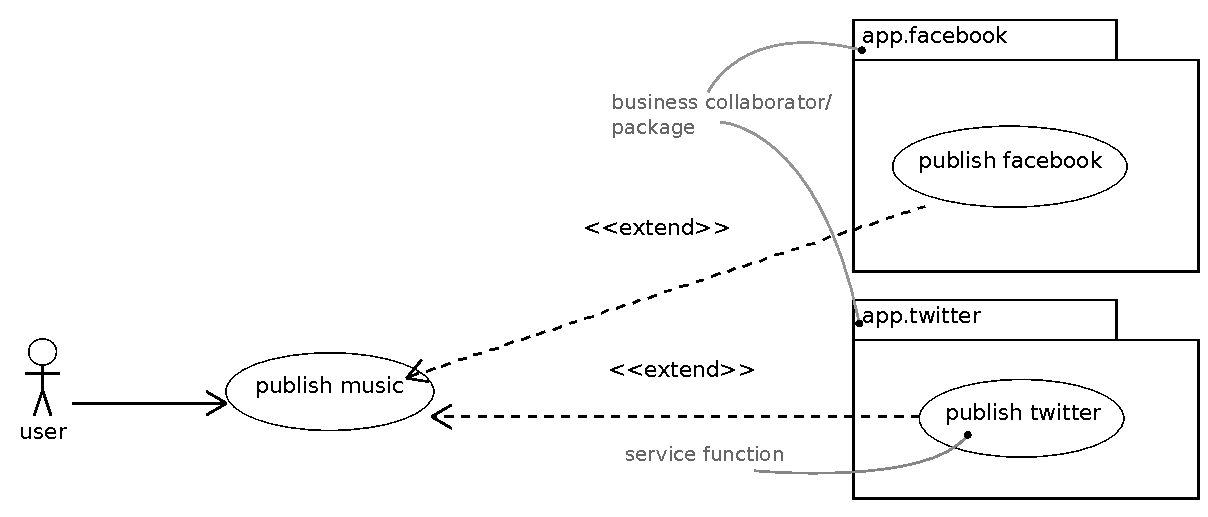
\includegraphics[width=.75\textwidth]{chapters/methodology/figs/businessCollaborator.pdf}
\caption{Business Collaborator / Package Representation.}
\label{fig:businessCollaborator}
\end{figure}


The {\sc Non-Functional Requirement} and {\sc Non-Functional Attribute} concepts
are represented as part of description of {\sc Use cases} and {\sc Constraints}.
For model this concepts the designer will use special tags to represent them  (figures
\ref{fig:nfr_detail} and \ref{fig:nfa_detail}).

% In summary, the main concepts to
% be modelled at this level are: {\sc Constraints}, and its respective {\sc
% Constraint Type}, and all {\sc Non-Functional Attribute} and {\sc Non-Functional
% Requirement} associated to each {\sc Constraint}. These concepts are not
% modelled in the original SOD-M extended use case model. Thus, we add these
% constraint concepts in the \textit{$\pi$-UseCase} model.

An {\sc Use Case} may have several {\sc Constraints}. Each
{\sc Constraint} has its name, description, and which ones should be
checked during the execution of the application. Each {\sc Constraint} is
represented as a stereotyped (\texttt{<<constraint>>}) use case. A
restriction may be a restriction on data ({\sc Value Constraint}),
represented as the stereotype \texttt{<<value>>}  (figure
\ref{fig:constraint_detail}); or on business rules (\textit{Business Constraint}), represented as the stereotype
\texttt{<<business>>}; and {\sc Exceptional Behaviour} constraints, which
represents constraint violation for the use case execution, represented as the stereotype
\texttt{<<exceptional\_behaviour>>}. 

The \textit{$\pi$-UseCase} meta-model
also represents the use of include and extend relations among the different use
cases identified. The semantics are the same as in the traditional UML use case
model. An include relation specifies the existence of a flow of events in which
the base use case includes the behaviour of the other use case and an extend
relation specifies that the behaviour of a base use case can be optionally
extended by the behaviour of another use case.
 

 \subsubsection{UML Concepts Representation} 
  

\begin{figure}[ht!]
\centering
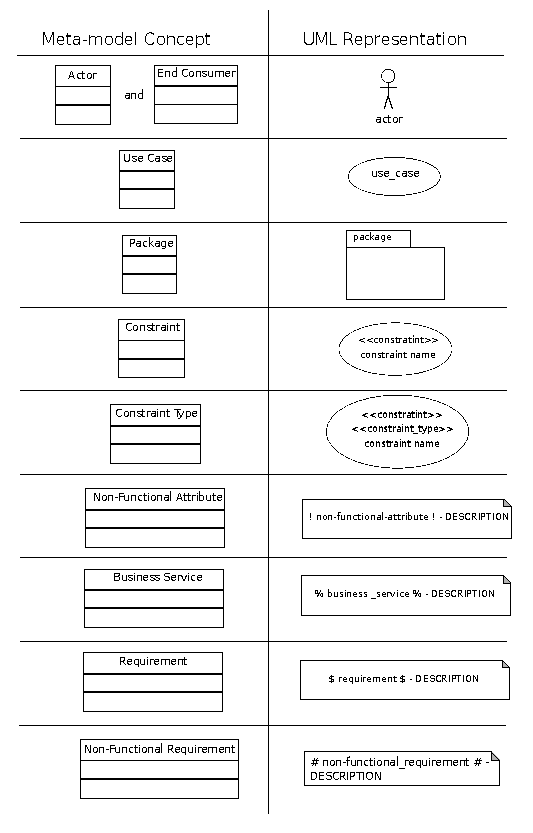
\includegraphics[width=0.65\textwidth]{chapters/methodology/figs/umlRepresentation.pdf}
\caption{\textit{$\pi$-UseCase} Concepts Represented as UML Elements.}
\label{fig:umlrepresentation}
\end{figure}

Once described the meaning of each \textit{$\pi$-UseCase} concept in the
meta-model, it is important to know how specific models can be
created from this general representation. Every \textit{$\pi$-UseCase} model
created to describe application features must follow the
meta-model concepts. The \textit{$\pi$-UseCase} meta-model describes what can be
specified in each model.

\begin{figure}[ht!]
  \centering
  \subfloat[\textit{Use Case} and \textit{Actor} Model]
  {\label{fig:piusecase1}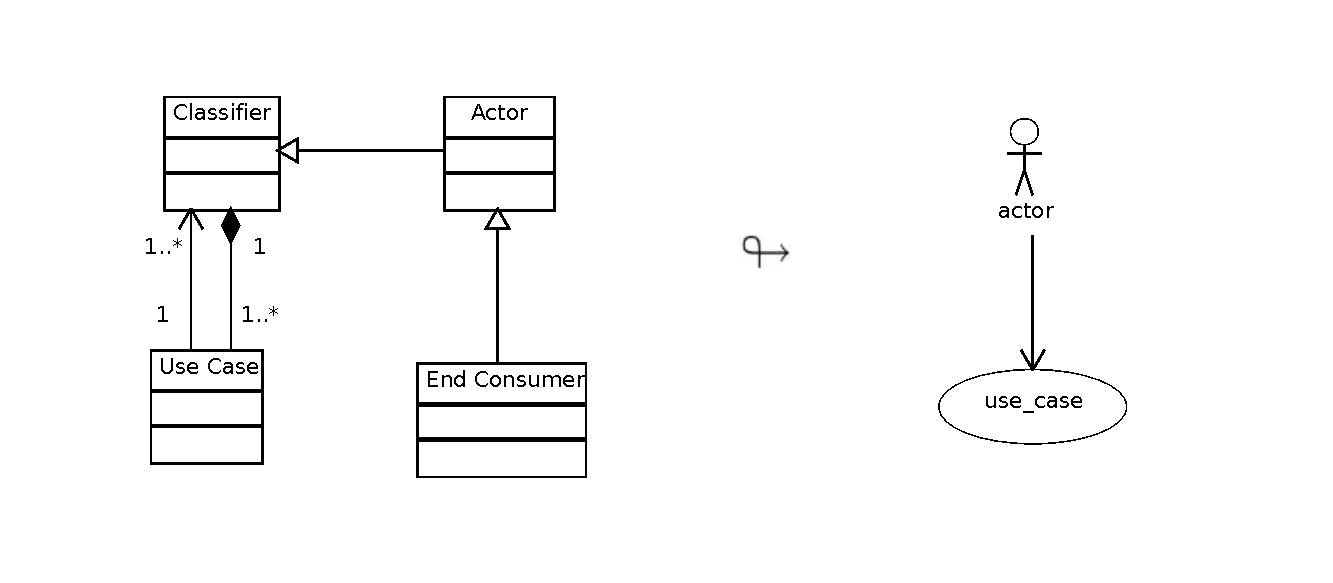
\includegraphics[width=0.8\textwidth]{chapters/methodology/figs/piusecase/pi_uc_usecase-actor_final}}
   %add desired spacing between images, e. g. ~, \quad, \qquad etc. (or a blank line to force the subfig onto a new line)
  ~
  \\
   \subfloat[\textit{Extended Use Case} Model]
  {\label{fig:piusecase2}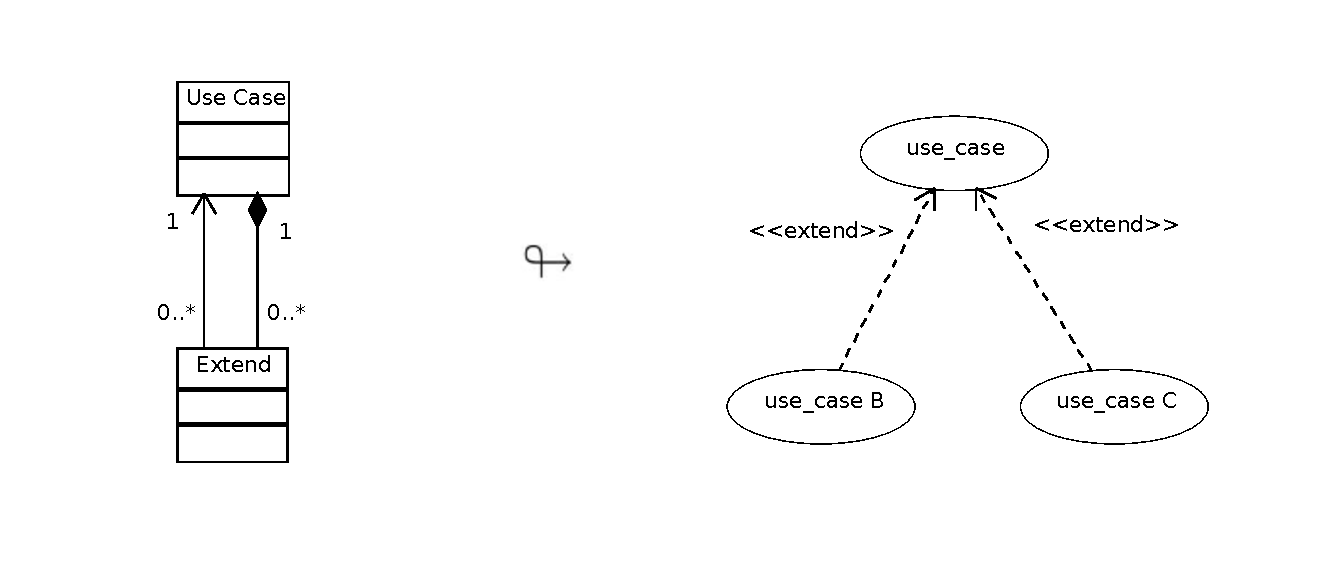
\includegraphics[width=0.8\textwidth]{chapters/methodology/figs/piusecase/pi_uc_extend_final}}
  ~ %add desired spacing between images, e. g. ~, \quad, \qquad etc. (or a blank line to force the subfig onto a new line)
  \\
 \subfloat[\textit{Include Use Case} Model]
  {\label{fig:piusecase3}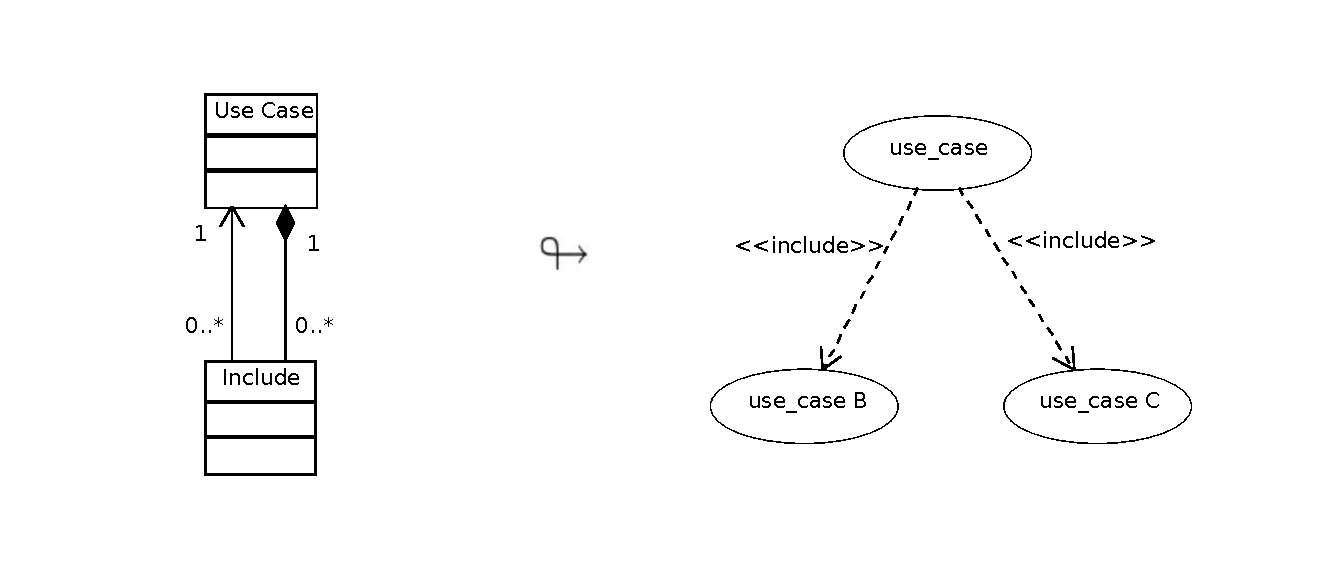
\includegraphics[width=0.8\textwidth]{chapters/methodology/figs/piusecase/pi_uc_include_final}}
   %add desired spacing between images, e. g. ~, \quad, \qquad etc. (or a blank line to force the subfig onto a new line)
  ~
  \caption{\textit{$\pi$-UseCase} Model Representation.}
  \label{fig:piuse_representation1}
\end{figure}

\begin{figure}[ht!]
  \centering
  \subfloat[\textit{Package} Model]
  {\label{fig:piusecase4}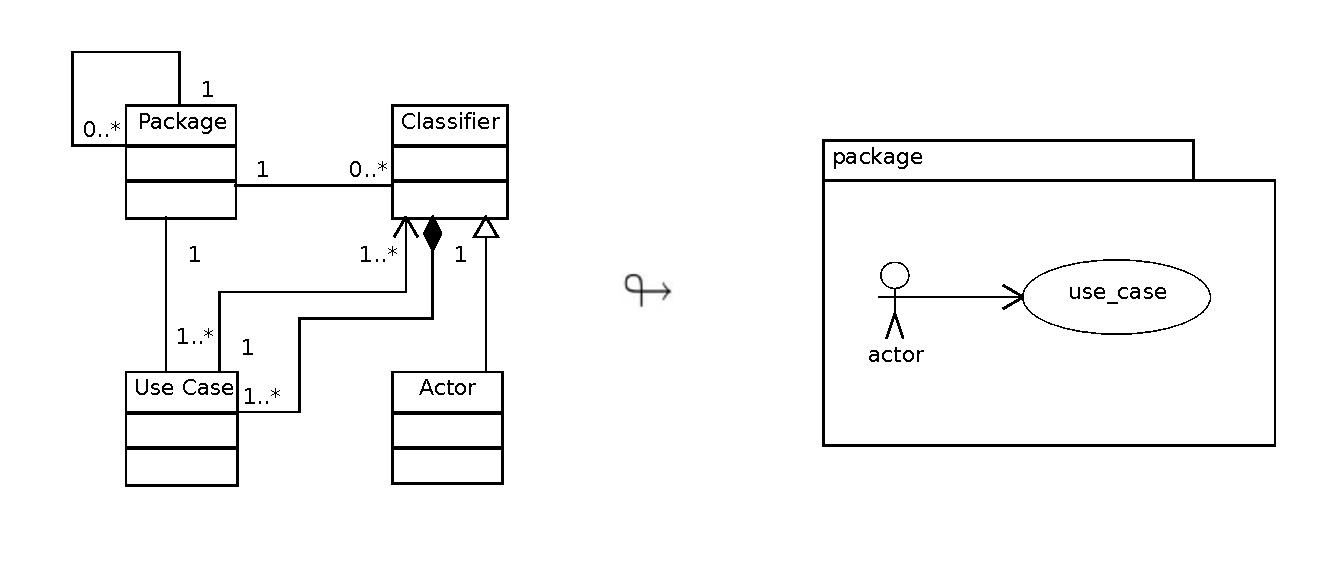
\includegraphics[width=0.8\textwidth]{chapters/methodology/figs/piusecase/pi_uc_package_final}}
  ~ %add desired spacing between images, e. g. ~, \quad, \qquad etc. (or a blank line to force the subfig onto a new line)
  \\
  \subfloat[\textit{Use Case}, \textit{Requirement} and
  \textit{Non-Functional Requirement} Model]
  {\label{fig:piusecase5}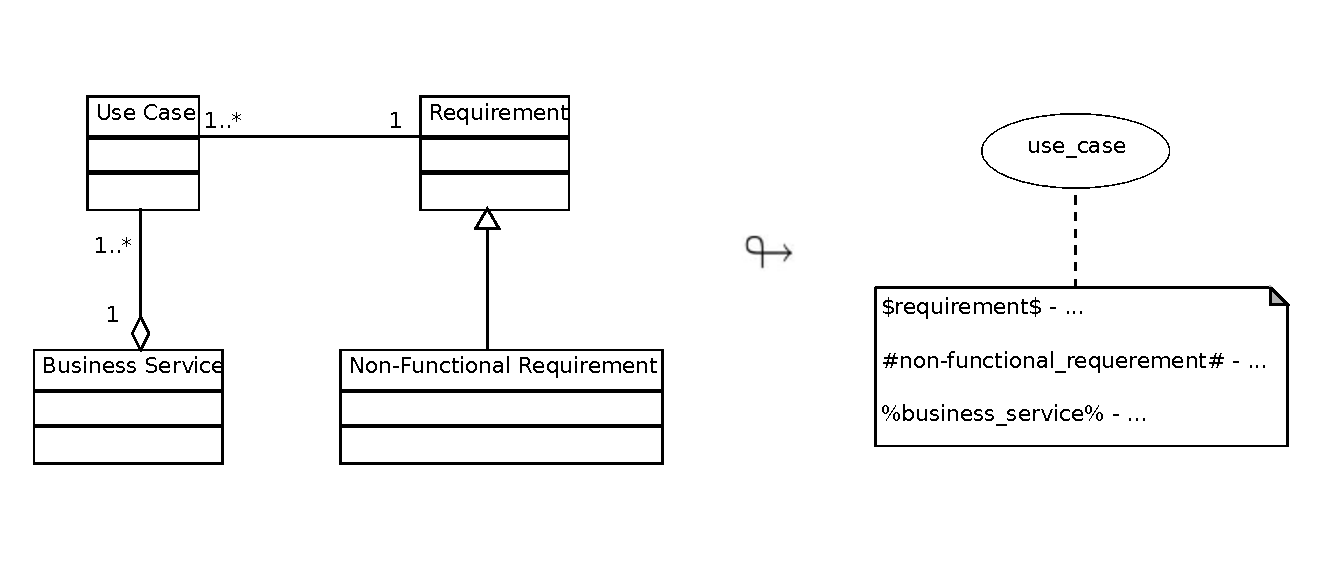
\includegraphics[width=0.8\textwidth]{chapters/methodology/figs/piusecase/pi_uc_usecase-comments_final}}
   %add desired spacing between images, e. g. ~, \quad, \qquad etc. (or a blank line to force the subfig onto a new line)
  ~
  \\
  \subfloat[\textit{Constraint} Model]
  {\label{fig:piusecase6}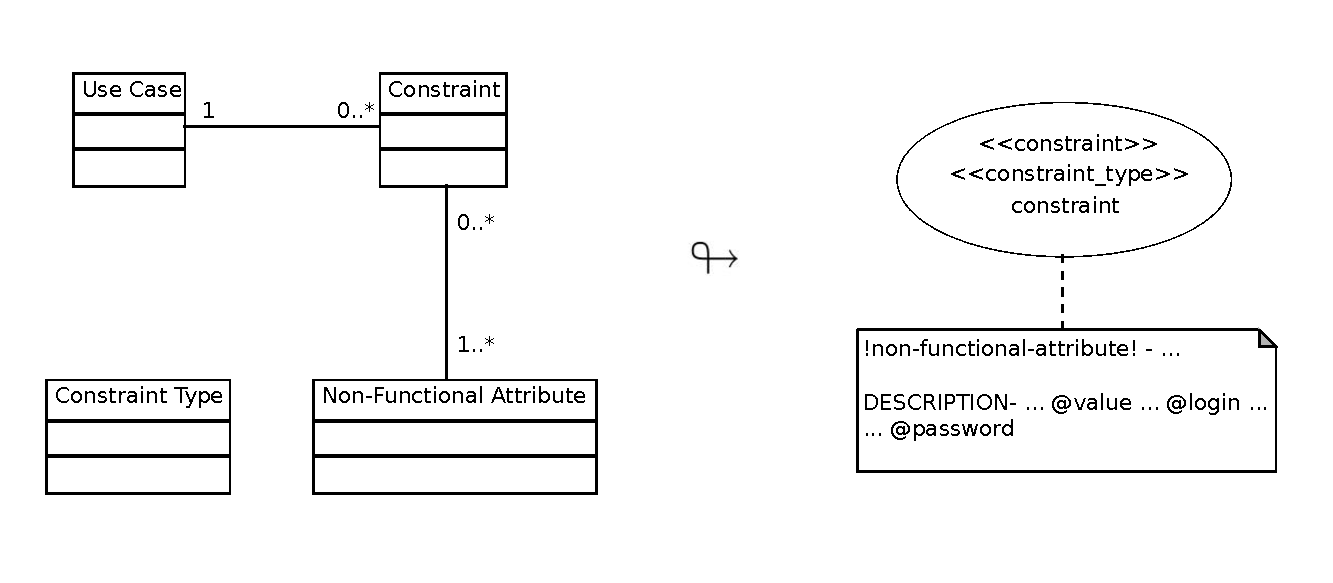
\includegraphics[width=0.8\textwidth]{chapters/methodology/figs/piusecase/pi_uc_constraint_final}}
  ~ %add desired spacing between images, e. g. ~, \quad, \qquad etc. (or a blank line to force the subfig onto a new line)

  \caption{\textit{$\pi$-UseCase} Model Representation (2).}
  \label{fig:piuse_representation2}
\end{figure}


The \textit{$\pi$-UseCase} concepts are modelled as described in
figure \ref{fig:umlrepresentation} and the relationship between these concepts
is also applied to the UML elements. Figures \ref{fig:piuse_representation1} and
\ref{fig:piuse_representation2} detail how to represent the relationship
between the meta-model concepts in a \textit{$\pi$-UseCase} model. 

The \textit{loop arrow} symbol ($\looparrowright$) is used in figures
\ref{fig:piuse_representation1} and \ref{fig:piuse_representation2} to
relate the concepts of the meta-model and the UML elements used in the
representation of the concepts.

\correctingText{This means how the \textit{$\pi$-UseCase} meta-model concepts (left
side) can be modelled as an UML model (right side).}


An {\sc Actor} is an abstraction of the {\sc End
Costumer} concept, presented in $\pi$SOD-M meta-model. Thus, it is possible to
associate several {\sc Actors} with an {\sc Use Case} and many {\sc Use Cases} with an {\sc
Actor} ({\sc End Costumer}). The original use case meta-model defines
that {\sc Classifier} is a superclass of {\sc Actor}. A {\sc Classifier} is a
category of UML elements that have some common features, such as
\textit{attributes} or \textit{methods}. The relationship between these entities
is many to many (figure \ref{fig:piusecase1}). An  {\sc Use Case} can also be
related with an {\sc Extends} or an {\sc Include} entity in the \textit{$\pi$-UseCase} model, and
this model preserve the original UML standard semantic. {\sc
Extends} and {\sc Include} are types of stereotyped dependence relationships
(\texttt{<<extend>>} and \texttt{<<include>>} in figures \ref{fig:piusecase2}
and \ref{fig:piusecase3}, respectively). The {\sc Extends} relationship can modify the behaviour of the base use case. Suppose someone
wants to close a bank account, however still have some money there. Before
closing the account, there should be a withdrawal or transfer of money in this
account, so that the balance is zero. This process is modelled with a {\sc
Extends} dependence between the \textit{close account} use case and
the \textit{withdrawal money} and \textit{transfer money} use cases. The {\sc Include} relationship includes
the steps from one use case into another.

A {\sc Package} clause and its relationship with {\sc Use Case} and {\sc Actor}
 can be modelled in \textit{$\pi$-UseCase} model. The original semantics was
 preserved and it is possible have different levels of packages, due to  {\sc
 Package} entity auto reference, one to many. Each package can have many use
 cases and actors (\ref{fig:piusecase4}).

The {\sc Requirements}, {\sc Non-Functional Requirements} and {\sc Business
Services} must be associated with a specific {\sc Use Case}. At this level of modelling, these information are represented as
comment \textit{tags}, they are: \textit{\$ \ldots \$} for {\sc Requirements},
\textit{\# \ldots \#} for {\sc Non-Functional Requirements}, and \textit{\%
\ldots \%} for {\sc Business Service}. A {\sc
Business Service} is a aggregation of {\sc Use Case}, and each {\sc Use Case}
must be related with a system requirement {\sc Requirements}. Figure
\ref{fig:piusecase5} presents the relationship of this concepts, and how
represent this information in UML.

All {\sc Use Cases} may also be associated with a set of {\sc Constraints}. A
{\sc Constraint} is a stereotyped use case that describes the {\sc Constraint Type} and its
restriction. Additional information is given by comment tags, \textit{!
\ldots !} for {\sc Non-Functional Attribute}, and \textit{@
\ldots @} for candidate variables or values that must be checked during the
system execution, as presented in figure \ref{fig:piusecase6}. The relationship
between {\sc Use Cases} and  {\sc Constraint} is made by a non-stereotyped
dependence arrow.


 
\subsubsection{\textit{To Publish Music} Use Case}

Considering the example scenario, the ``\textit{To Publish Music}'' use case can
update the Facebook or Twitter user status. Therefore, it is necessary to
perform a social network authentication with the user's data. Each social
network uses different services and different forms of authentication. The
\textit{authentication} constraint is required to update a music status. The
restriction is stereotyped as a \texttt{<<value>>} constraint, because the
\textit{user's id} and \textit{password} are verified. The {\sc Non-Functional
Requirement} that is being modelled for this use case is \textit{Security},
because, considering  table \ref{tab:result04}, ``\textit{authentication}'' is
a {\sc Non-Functional Attribute} of \textit{Security}. These information will be
refined and detailed in the following phases.

 
% 
% \begin{figure}[ht!]
% \centering
% 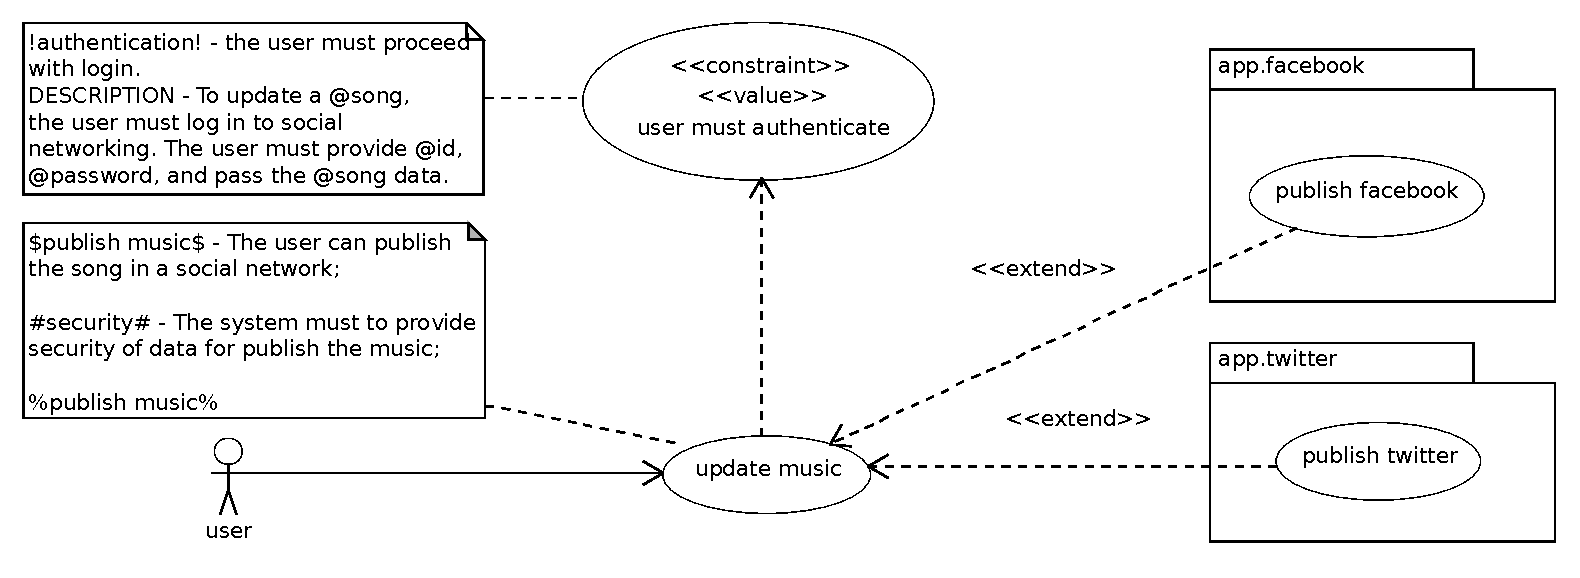
\includegraphics[width=.9\textwidth]{chapters/methodology/figs/piusecase/application/packages}
% \caption{$\pi$-UseCase Scenario Example.}
% \label{fig:usecasemodelpackages}
% \end{figure}



Figure \ref{fig:usecaseContraint} shows
the model represented in figure \ref{fig:example_usecase} for the \textit{buy
music, download music, listen music} and \textit{pay} use cases. The model was
designed considering the meta-model representation detailed in figures
\ref{fig:piuse_representation1} and \ref{fig:piuse_representation2}, and also
the \textit{$\pi$-UseCase} meta-model. Notice that from  \textit{$\pi$-UseCase}
concepts is possible to describe the actors, use cases, constraints,
non-functional requirements and their attributes. For example, the \textit{pay}
use case (figure \ref{fig:usecaseContraint}), there are extended use cases, constraints, packages, non-functional requirements and non-functional
attributes related to this function. The modeling was based on the described
representation of the \textit{$\pi$-UseCase} meta-model. The extended use case
representation presented in figure \ref{fig:piusecase2} is used in the model to
expressed the \textit{pay by PayPal} and \textit{pay by card} extended use
cases. The include use case representation presented in figure \ref{fig:piusecase3} is
used in the model to express the included relation of \textit{buy music} and
\textit{pay} use cases. The package representation presented in figure
\ref{fig:piusecase4} is expressed in the example by the \textit{app.bank}
package and the \textit{pay} use case relation. The representation described in figures
\ref{fig:piusecase5} and \ref{fig:piusecase6} is expressed by the \textit{pay}
use case properties' description. The combination of a \textit{$\pi$-UseCase}
meta-model's entities means that all entities presented in figures
\ref{fig:piUseCaseExample} and \ref{fig:usecaseContraint} can be modelled to
express the quality requirements.

The use cases that have restrictions are \textit{buy music} and
\textit{pay}. The process of buying a song requires the user's private data
for a Spotify account, and also a secure connection, represented as
\texttt{<<value>>} and \texttt{<<business>>} constraint, respectively. For
payment, the user must provide the data of payment card or PayPal account login
and password, represented as \texttt{<<value>>} stereotype . Other restriction
is that the minimum payment value is 2 euros. The {\sc Non-Functional
Requirement} that are being modelled for this use cases are \textit{Security}
and \textit{Reliability}. The specific {\sc Non-Functional Attributes} for this
restriction is \textit{Transaction} and \textit{Confidentiality} (see figure
\ref{fig:usecaseContraint}).


\begin{figure}[ht!]
\centering
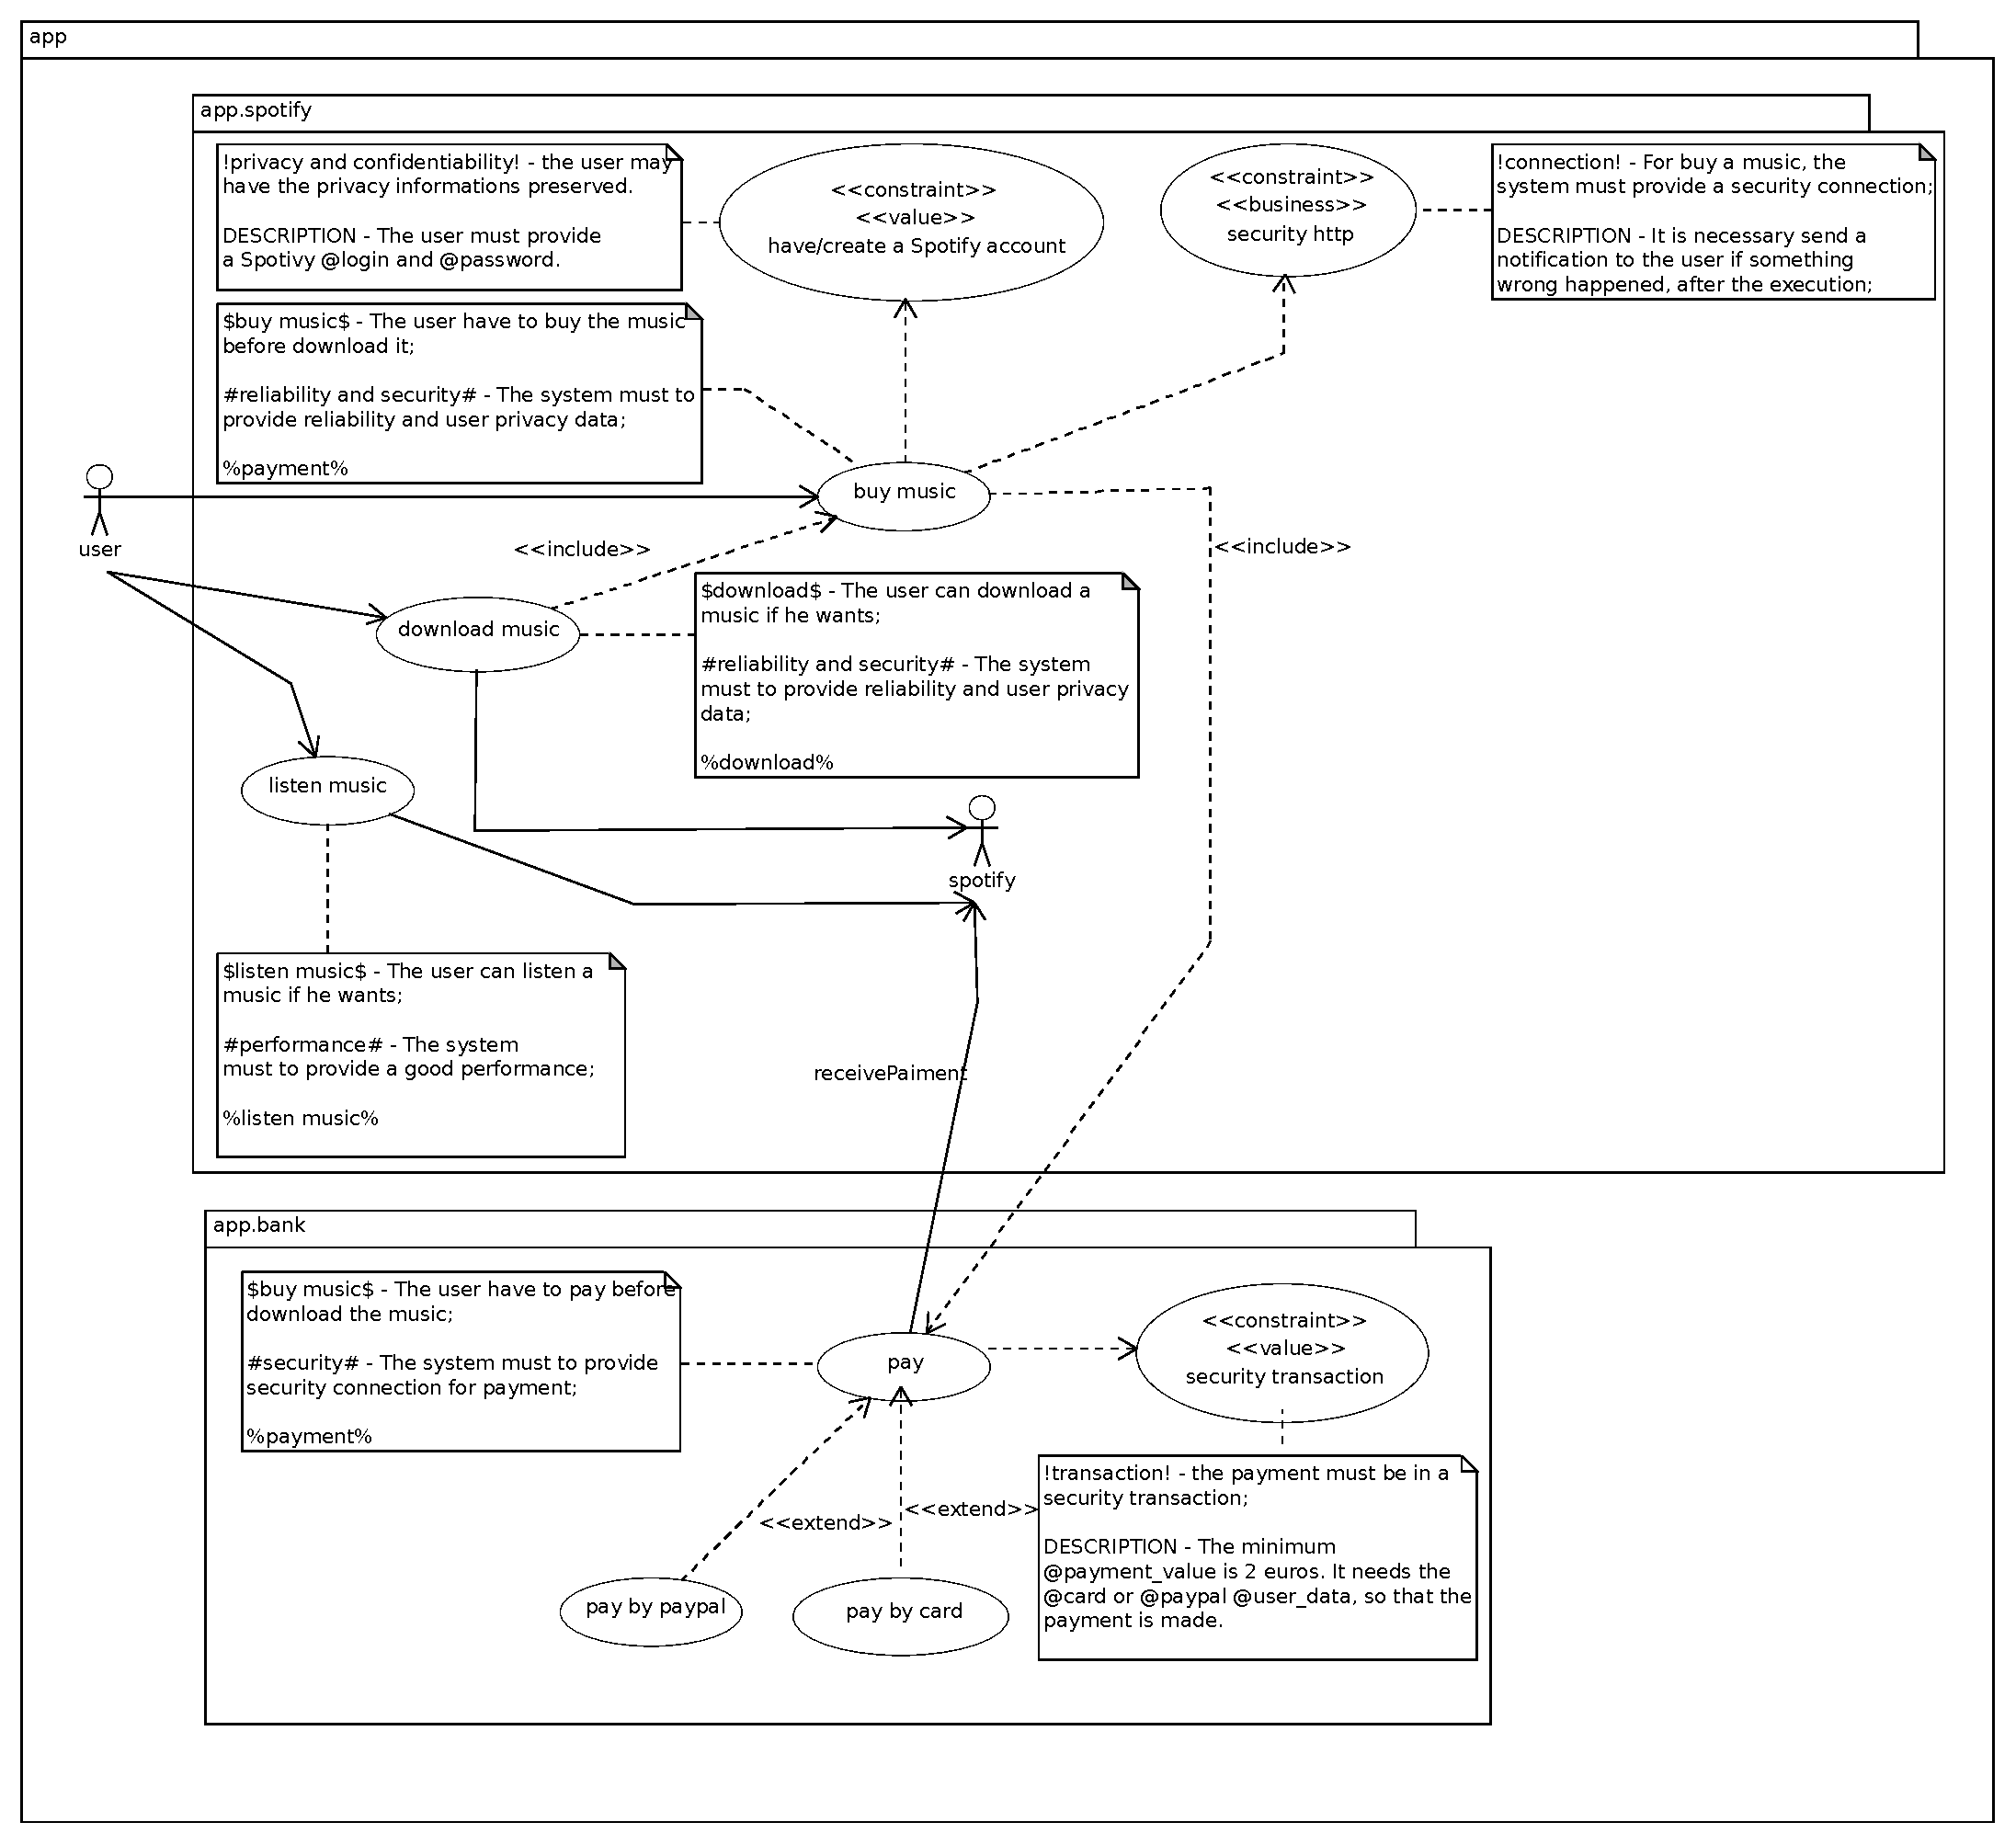
\includegraphics[width=.99\textwidth]{chapters/methodology/figs/piusecase/application/packages2.pdf}
\caption{Use Case Model With Constraint Definition - Scenario Example Refined.}
\label{fig:usecaseContraint}
\end{figure}

% Each {\sc Constraint} may be related to {\sc Non-Functional
% Attributes}. These types are the attributes related to {\sc Non-Functional
% Requirement}. For example, \textit{security} is an {\sc Non-Functional Requirement} that
% comprises attributes such as \textit{Confidentiality} and \textit{Privacy}
% ({\sc Non-Functional Attribute}). Thus the use case constraints are always
% related to a {\sc Non-Functional Requirement} (figure
% \ref{fig:usecasemodel}).

\bigskip
\bigskip

After modeling the system services and features, and its
restrictions, it is necessary to model the services process and its
execution restrictions. For this, the methodology uses a service process diagram
to describe the services execution and contracts. Next we present the
\textit{$\pi$-ServiceProcess} model. This model refines the application
constraints through the workflow model \correctingText{(as presented in Figure
\ref{fig:developmentProcess})}.

\subsection{\textit{$\pi$-ServiceProcess} Model}


A \textit{Service Process} is a collection of related, structured activities that produce a specific service or product for
a particular customer. It can be visualized with a flowchart
as a sequence of activities with interleaving decision points.  A set of
linked activities that take an input and transform it to create an output.
Ideally, the transformation that occurs in the process should add value to the
input and create an output that is more useful and effective. To represent these
properties our methodology proposes the \textit{$\pi$-ServiceProcess} model.

% The main difference between the service process diagram proposed by SOD-M
% \cite{valeriaThesis} and our \textit{$\pi$-ServiceProcess}  diagram is the
% inclusion of concepts that represent the modeling of non-functional
% requirements, as well as in \textit{$\pi$-UseCase} model. 
The non-functional requirements are specified in this model using the concepts
of contracts and assertions over functions. These contracts may represent the
control of privacy information, performance, reliability, and so on.

 \subsubsection{\textit{$\pi$-ServiceProcess} Diagram, Terms and Concepts} 

% In the context of reliable service composition development, the
% \textit{$\pi$-ServiceProcess} perform different third party functions services,
% so that something new can be offered. 

Systems that use third party services add value to the application because the
services are already available and validated. If the services do not offer any
quality warranty, these quality requirements are the responsibility of the
application designer. Thus, the contracts of services will be modeled as a
wrapper which describes restrictions on input and output information on
particular functions or a set of them. 


$\pi$SOD-M proposes modeling \textit{Service Process} diagram
(\textit{$\pi$-ServiceProcess} model), that is defined considering the
functional and non-functional requirements designed in a
\textit{$\pi$-UseCase} model.

The \textit{$\pi$-ServiceProcess} model represents the service processes and its
contracts. It models the set of system activities and describe contracts for
each activity or the process as a whole. Each service identified in the previous
model (\textit{$\pi$-UseCase}) is mapped to an action. 

% Figure \ref{fig:serviceprocess} shows
% the \textit{$\pi$ServiceProcess} meta-model proposed by $\pi$SOD-M method for
% model \textit{Service Process}.

 

%  \bigskip 
%  \textbf{Properties} 
%  \bigskip 
 
 
%  What differentiates this model
%  from others is its particular content and how to represent restrictions to be
%  verified during the workflow execution.
%  
  \begin{figure}[ht!]
\centering
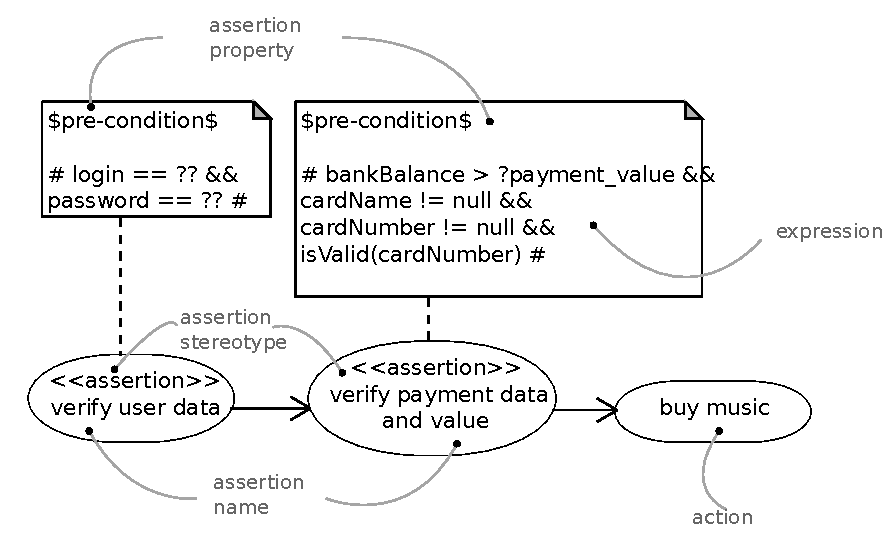
\includegraphics[width=.8\textwidth]{chapters/methodology/figs/assertion_detail.pdf}
\caption{Assertion Representation.}
\label{fig:assertion_representation}
\end{figure}
 
 
 A \textit{$\pi$-ServiceProcess} model represents the system process,
 actions, assertions and contracts. This model describes the workflow for the modelled application
 behaviour. The behaviour is represented by each action and the restrictions by
 the assertion description. All assertions are described by stereotyped actions.
 
  
 
   \begin{figure}[ht!]
\centering
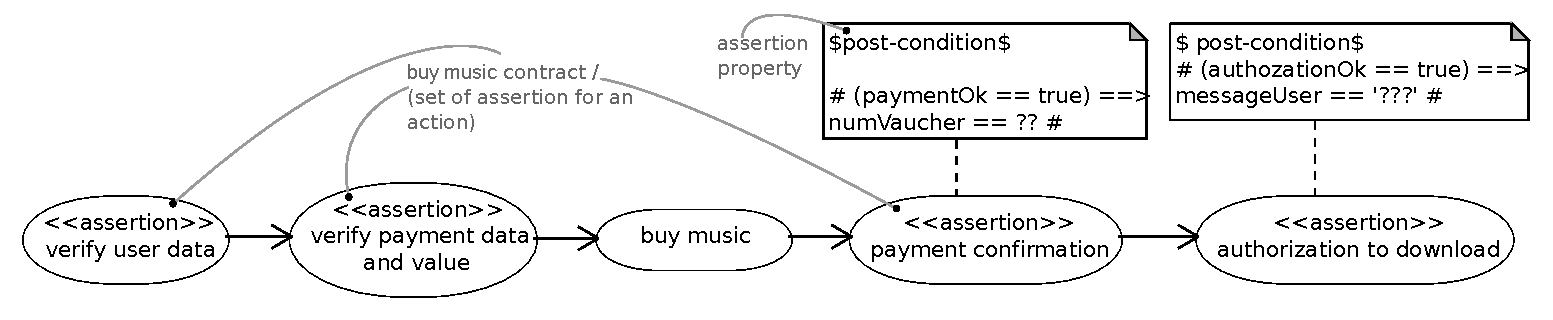
\includegraphics[width=.99\textwidth]{chapters/methodology/figs/contract_detail.pdf}
\caption{Contract Representation.}
\label{fig:contract_representation}
\end{figure}

Figures \ref{fig:assertion_representation} and \ref{fig:contract_representation}
present the assertion and contract representation in this
model. An Assertion is represented in UML, and a set of assertions forms a
contract. Assertions describe restrictions on a single action, but actions may
have different restrictions. Figure \ref{fig:assertion_representation} shows how an assertion is modelled, with their property type, name and acceptable values (expressed through
expressions), while figure \ref{fig:contract_representation} shows how this set
of assertions form a single action contract.     

   \begin{figure}[ht!]
\centering
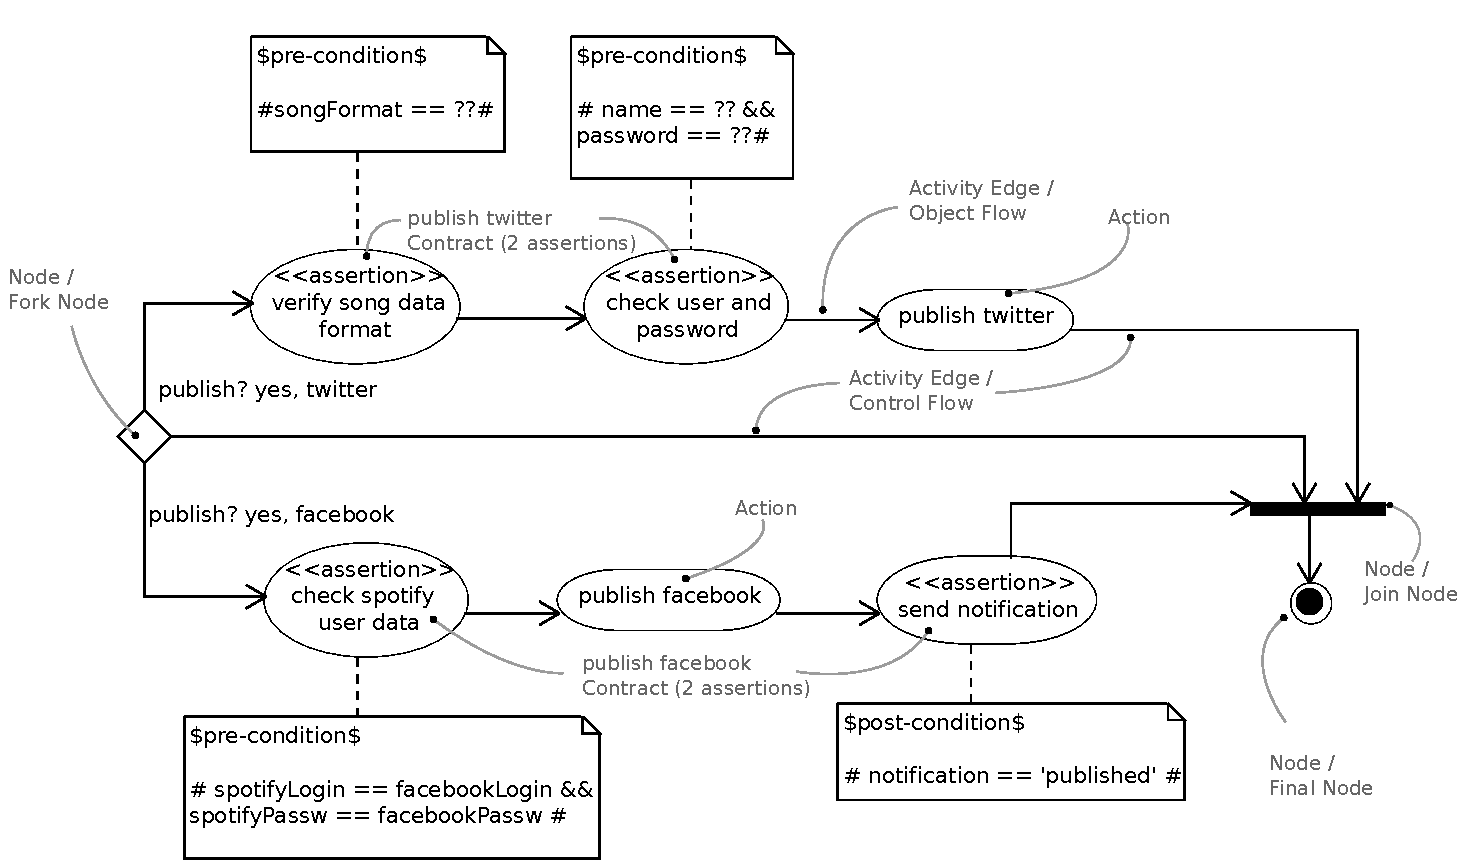
\includegraphics[width=.99\textwidth]{chapters/methodology/figs/otherObjects_detail.pdf}
\caption{Node, Activity Edge and Contract Representation.}
\label{fig:other_representation}
\end{figure}

Figure \ref{fig:other_representation} shows the representation of the general
concepts of this model, nodes, activity edges, actions and contracts. This figure also refines the information
for publish a song in a social network.
  

 \subsubsection{Meta-model} 


Considering the $\pi$SOD-M concepts (figure \ref{fig:pisodm-concepts}), the
\textit{$\pi$-ServiceProcess} meta-model (figure \ref{fig:serviceprocess})
describes the system functionalities to be modelled in a contract based service
process. The $\pi$SOD-M concepts modelled in the \textit{$\pi$-ServiceProcess}
meta-model are: {\sc Contract, Assertion, Exceptional Behaviour, Activity,
Service Activity, Action} and {\sc Constraint}.
 


Restrictions on activities and services are not described in the
original SOD-M proposal. The concepts of {\sc Contract, Assertion} and
{\sc Exceptional Behaviour} make it possible to model restrictions on services
execution, ensuring greater reliability application. Entities highlighted in
\textit{$\pi$-ServiceProcess} meta-model (figure \ref{fig:serviceprocess})  are
the difference from the original SOD-M service process model.

 \begin{figure}[ht!]
\centering
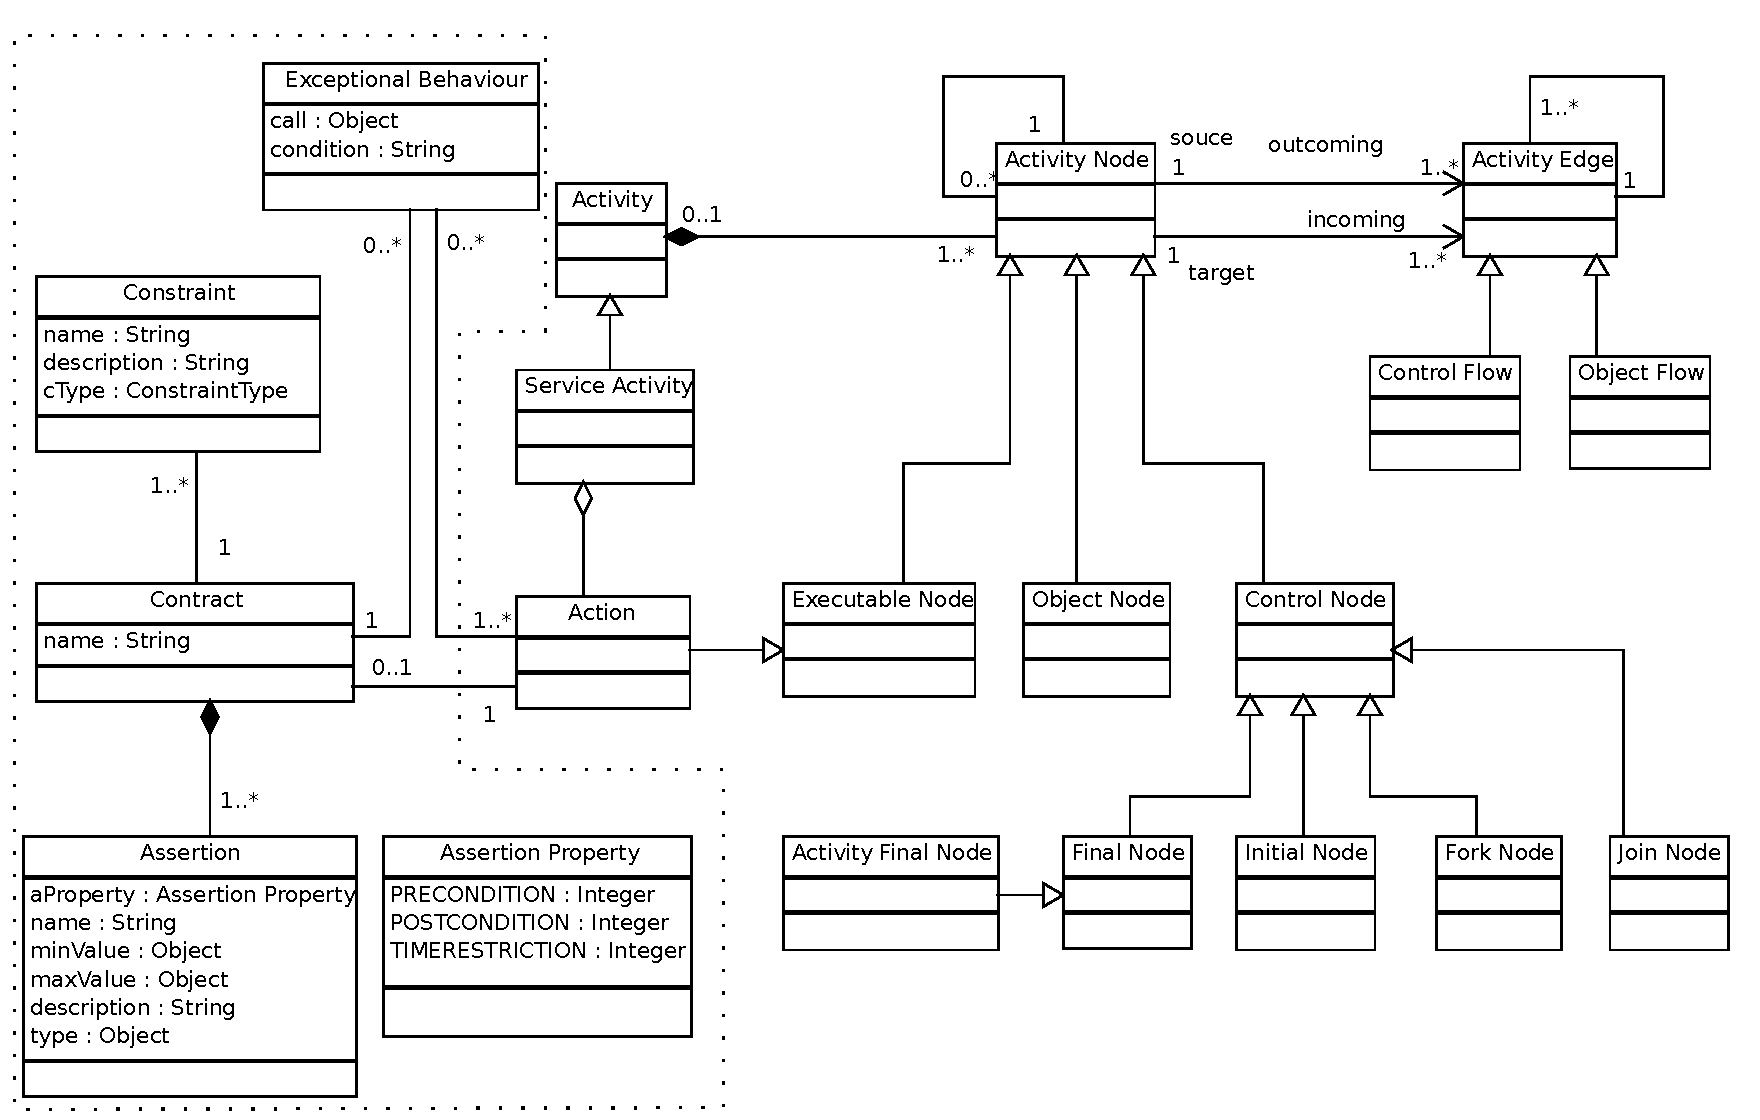
\includegraphics[width=1.0\textwidth]{chapters/methodology/figs/PiServiceProcess.pdf}
\caption{$\pi$-ServiceProcess Concepts (Meta-model).}
\label{fig:serviceprocess}
\end{figure}

A specific \textit{$\pi$-ServiceProcess} model shows the set of logically
related activities that need to be performed in a service-based system. So, the
activities of this model represent a behaviour that is part of the
system workflow. $\pi$SOD-M proposes representing this model using
the UML activity diagram, with an extension for {\sc Contract} design,
which encapsulates several {\sc Constraints} modelled in \textit{$\pi$-UseCase}
model. In \textit{$\pi$-ServiceProcess}, three main features are
represented: (i) \textit{service process}, (ii) \textit{service activity} and
(iii) \textit{activity contract}. The service process is represented by the
model itself. A service activity represents a behaviour that is part of the
execution flow, and is identified in this model as an {\sc Action}. A activity
contract represents the {\sc Non-Functional Requirement} behaviour that is also
part of the execution flow of a service, and is identified in this model as an
stereotyped activity (\texttt{<<assertion>>}). All {\sc Assertion} related with
an {\sc Action} compose a {\sc Contract}. From the {\sc Contract} and {\sc
Assertion} concepts is possible to define the interface specifications
for each activity service, such as pre-conditions and post-conditions.

\subsubsection{UML Concepts Representation} 
  
  
To formalize the concept of {\sc Contract} by rules, we use the definition of
{\sc Assertion} (figure \ref{fig:pisp1}). An {\sc Assertion} is represented by a
stereotyped action (\texttt{<<assertion>>}), and {\sc Assertion Properties}
through comments. An {\sc Assertion} may be a \textit{pre-condition},
\textit{post-condition} or a \textit{time restriction} over the service
execution ({\sc Assertion Property}). These information are represented as
the comment \textit{tags} \textit{\$ \ldots \$}. The assertion predicate is
modelled as \textit{\# \ldots \#} tag. Figure \ref{fig:pisp1} shows how these
concepts are represented in UML.



\begin{figure}[ht!]
  \centering
  \subfloat[\textit{Assertion} Model]
  {\label{fig:pisp1}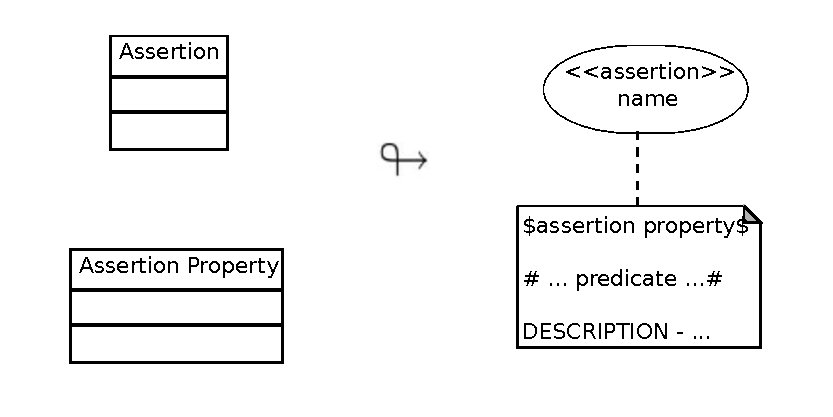
\includegraphics[width=0.5\textwidth]{chapters/methodology/figs/piserviceprocess/assertion_final}}
  ~ %add desired spacing between images, e. g. ~, \quad, \qquad etc. (or a blank line to force the subfig onto a new line)
  \subfloat[\textit{Contract} Model]
  {\label{fig:pisp2}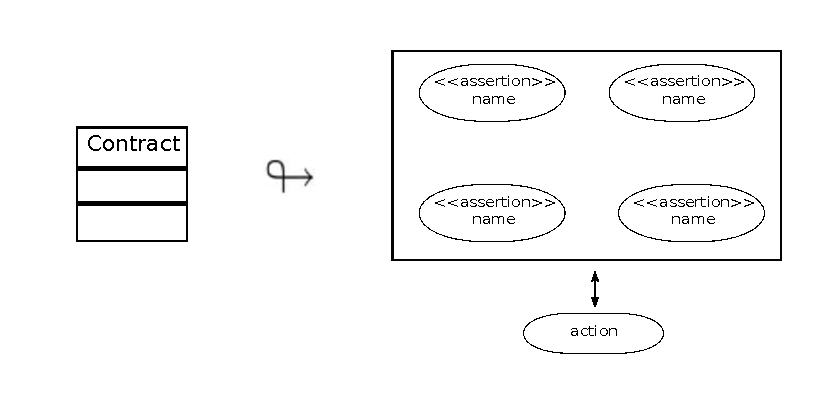
\includegraphics[width=0.5\textwidth]{chapters/methodology/figs/piserviceprocess/contract_final}}
   %add desired spacing between images, e. g. ~, \quad, \qquad etc. (or a blank line to force the subfig onto a new line)
  \\
  \subfloat[\textit{Exceptional Behaviour} Model]
  {\label{fig:pisp3}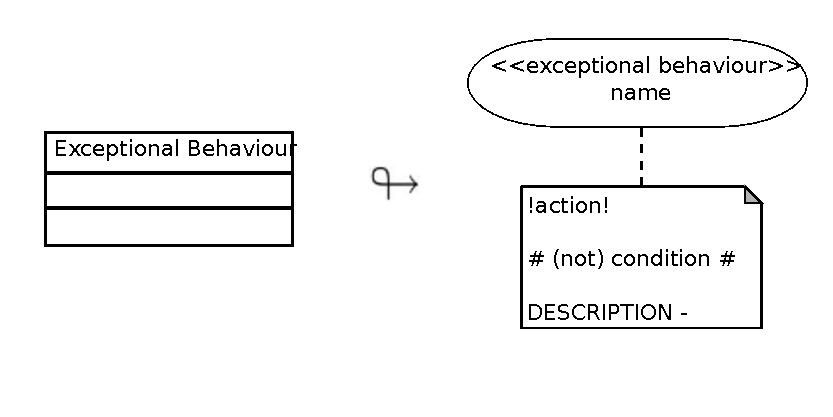
\includegraphics[width=0.5\textwidth]{chapters/methodology/figs/piserviceprocess/exceptionalBeh_final}}
  ~ %add desired spacing between images, e. g. ~, \quad, \qquad etc. (or a blank line to force the subfig onto a new line)
  \subfloat[\textit{Action} Model]
  {\label{fig:pisp4}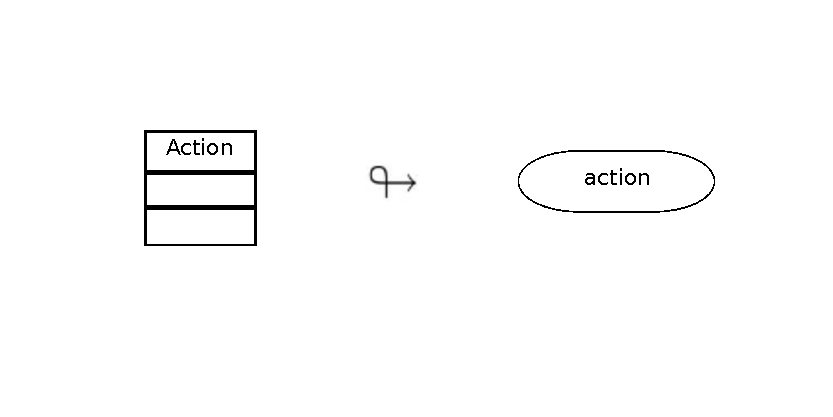
\includegraphics[width=0.5\textwidth]{chapters/methodology/figs/piserviceprocess/action_final}}
   %add desired spacing between images, e. g. ~, \quad, \qquad etc. (or a blank line to force the subfig onto a new line)
  \\
  \subfloat[\textit{Service Activity} Model]
  {\label{fig:pisp5}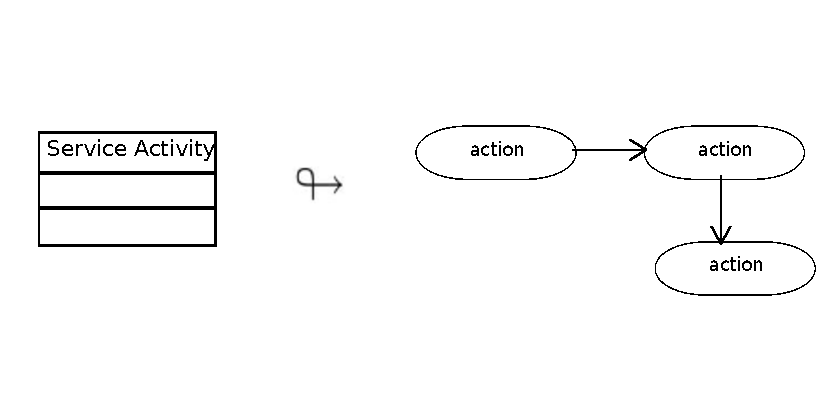
\includegraphics[width=0.5\textwidth]{chapters/methodology/figs/piserviceprocess/serviceActivity_final}}
  ~ %add desired spacing between images, e. g. ~, \quad, \qquad etc. (or a blank line to force the subfig onto a new line)

  \caption{\textit{$\pi$-ServiceProcess} Model Representation.}
  \label{fig:pisp_representation}
\end{figure}


\begin{figure}[ht!]
  \centering
  \subfloat[\textit{Control Nodes} Model]
  {\label{fig:pisp6}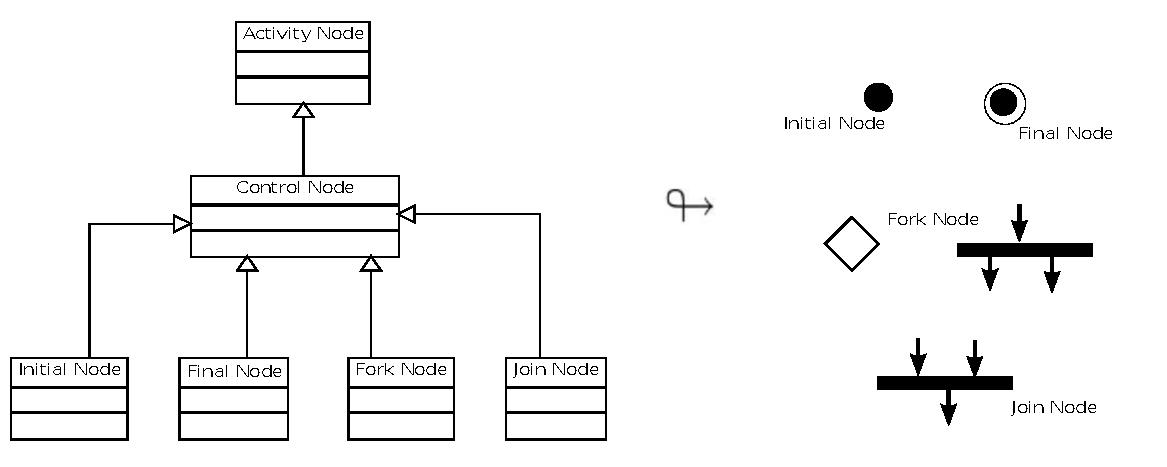
\includegraphics[width=0.8\textwidth]{chapters/methodology/figs/piserviceprocess/controlNode_final}}
  ~ %add desired spacing between images, e. g. ~, \quad, \qquad etc. (or a blank line to force the subfig onto a new line)
  \\
  \subfloat[\textit{Activity Edge - Control Flow} Model]
  {\label{fig:pisp7}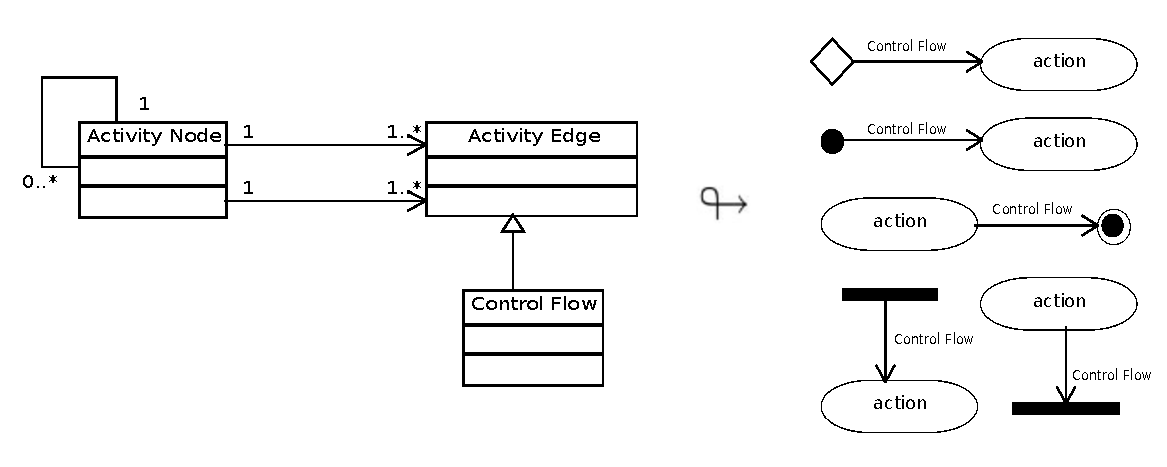
\includegraphics[width=0.8\textwidth]{chapters/methodology/figs/piserviceprocess/activityEdge_final}}
   %add desired spacing between images, e. g. ~, \quad, \qquad etc. (or a blank line to force the subfig onto a new line)
  ~
  \\
  \subfloat[\textit{Activity Edge - Control Object} Model]
  {\label{fig:pisp8}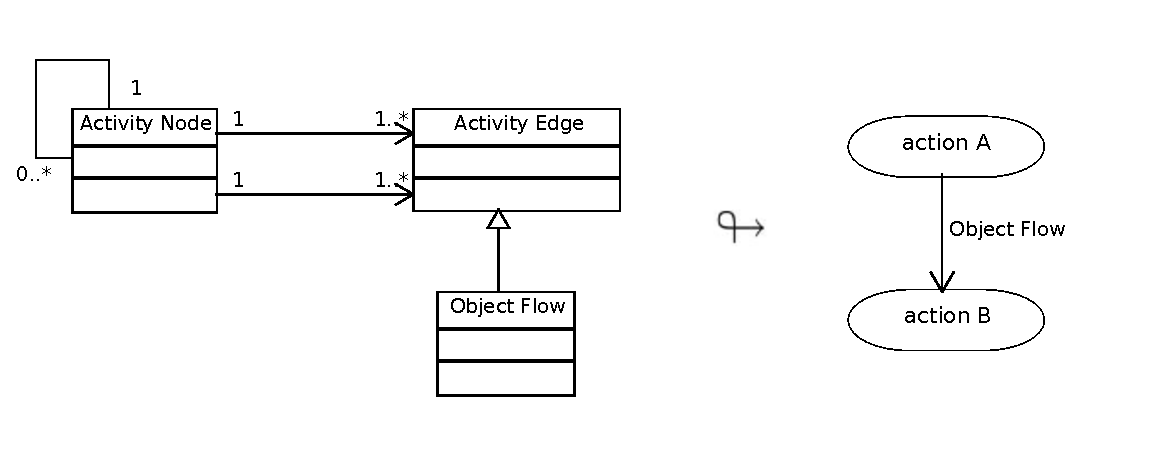
\includegraphics[width=0.8\textwidth]{chapters/methodology/figs/piserviceprocess/activityEdge2_final}}
  ~ %add desired spacing between images, e. g. ~, \quad, \qquad etc. (or a blank line to force the subfig onto a new line)

  \caption{\textit{$\pi$-ServiceProcess} Model Representation (2).}
  \label{fig:pisp_representation2}
\end{figure}



A set of {\sc Assertion} composes a service {\sc Contract} related with an {\sc
Action} (figure \ref{fig:pisp2}).  An Assertion describes a value (\textit{value
constraint} from $\pi$-UseCase model) restriction, setting maximum and minimum
limits, or business restrictions, setting conditions for function calls
((\textit{business constraint} from $\pi$-UseCase model)). The
business restrictions are defined over service functions. Every service contract
may have an exception behaviour, if a constraint is not obeyed. For example, if the
user card information are incorrect, the service is called again until the limit
of 3 calls, otherwise, execution continues normally. In this case, the exception
is the new call to the same service. For this, we also use the concept of {\sc
Exceptional Behaviour} (figure \ref{fig:pisp3}). A {\sc Exceptional Behaviour}
is also a stereotyped action (\texttt{<<exceptional behaviour>>}) and its
properties are modelled through comment tags. The condition to be verified is
modelled as \textit{\# \ldots \#} tag. Figure \ref{fig:pisp1} shows how these
concepts are represented in UML. If the condition is \textit{false}, the
predicate becomes true, because of the expression negation
(\textit{not}). Thus the action is performed. The action to be performed is
modelled as \textit{! \ldots !} tag. The {\sc Action} concept is modelled in UML
as the action component (figure \ref{fig:pisp4}), and a {\sc Service Activity}
represents a set of {\sc Action} (figure \ref{fig:pisp5}). 
We highlight the models in figures \ref{fig:pisp1}, \ref{fig:pisp2} and
\ref{fig:pisp3}, because they present how an assertion action, a contract, and a
exceptional behaviour can be designed.

Figure\ref{fig:pisp_representation2}
shows the UML representation of the {\sc Control Nodes} and {\sc Activity Edges}
concepts in $\pi$-ServiceProcess meta-model. This representation follows the
original UML specification. Figure \ref{fig:pisp6} presents the
{\sc Control Nodes} and how its can be applied in a real modelling, and finally
figures \ref{fig:pisp7} and \ref{fig:pisp8} show the {\sc Activity Edges} and
its application. 

% These model concepts is very important, because it is from
% the restrictions described in the previous model ($\pi$-UseCase) that each
% constraint begins to be refined and applied to real application services. 
 

\subsubsection{\textit{To Publish Music} Process}


Considering the example scenario, the contract based process of activities
execution is shown in figure \ref{fig:serviceprocessContract}.
The activities flow in figure \ref{fig:example_serviceprocess} presents any restriction. Thus, it is necessary
to represent each {\sc Constraint} modelled in a more representative {\sc
Contract} based service activity diagram.

Based on the concepts described and its representation in UML, we describe how
to model a service process using the assertions as restrictions for each action.
The difference of the model shown in figure \ref{fig:example_serviceprocess}
and the figure \ref{fig:serviceprocessContract} is that restrictions are added
on the actions in order to describe quality requirements.


\begin{figure}[ht!]
\centering
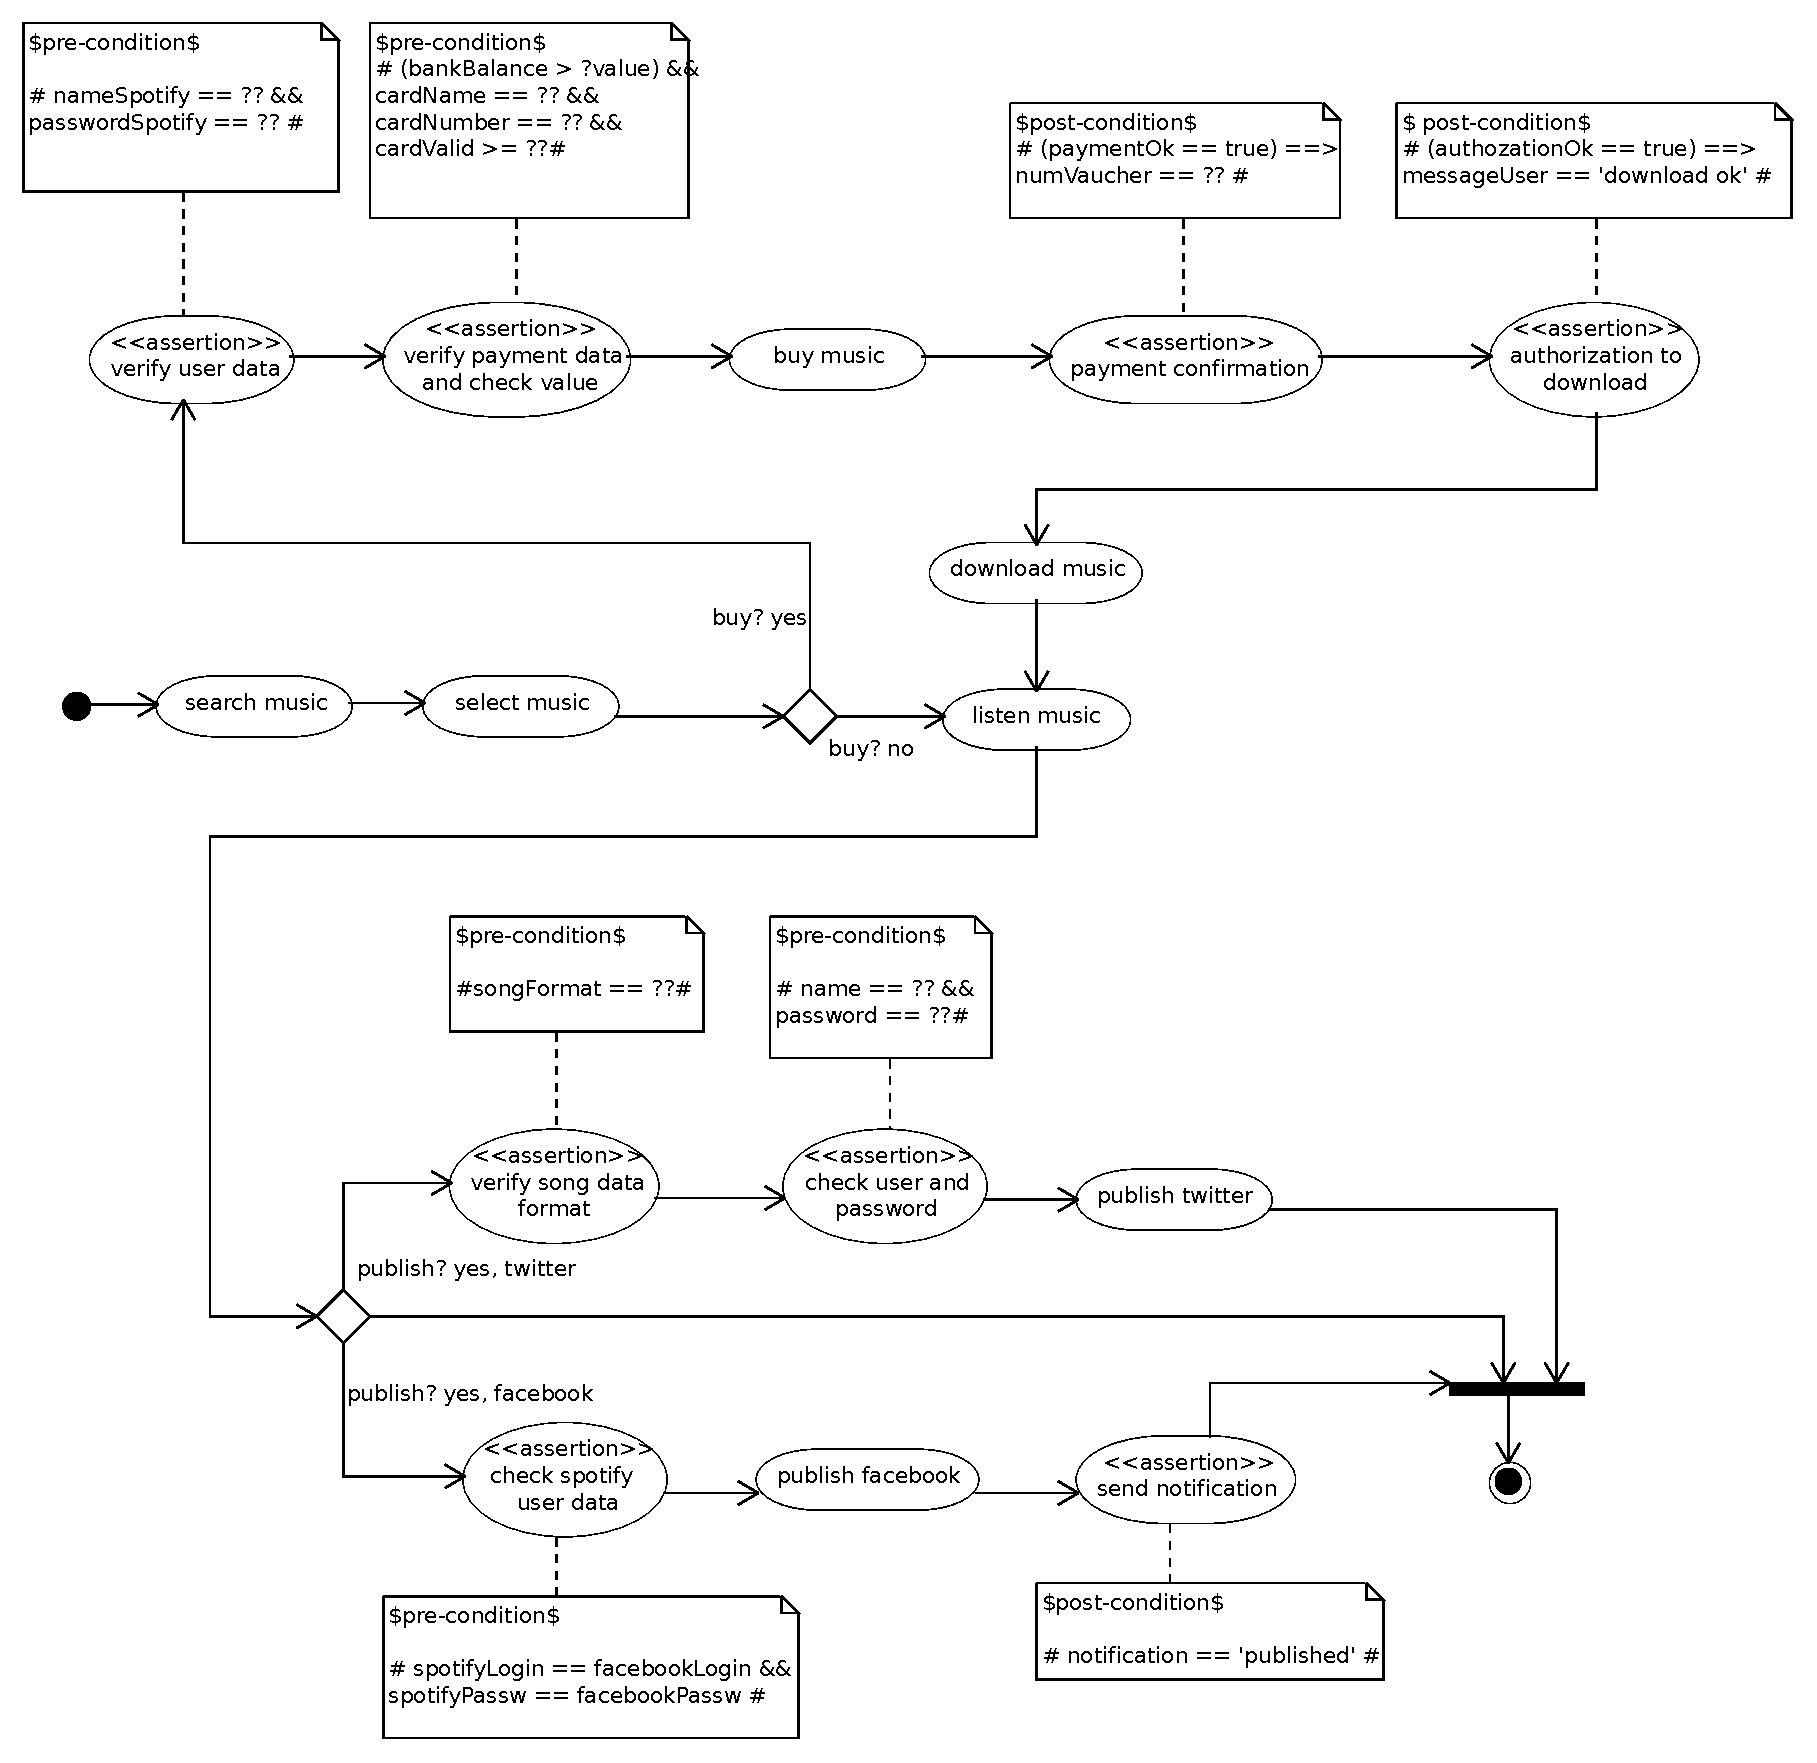
\includegraphics[width=.99\textwidth]{chapters/methodology/figs/piserviceprocess/runningExampleSP_final.pdf}
\caption{Service Process Model with Contract Definition - Complete Example.}
\label{fig:serviceprocessContract}
\end{figure}

% \begin{figure}[ht!]
% \centering
% 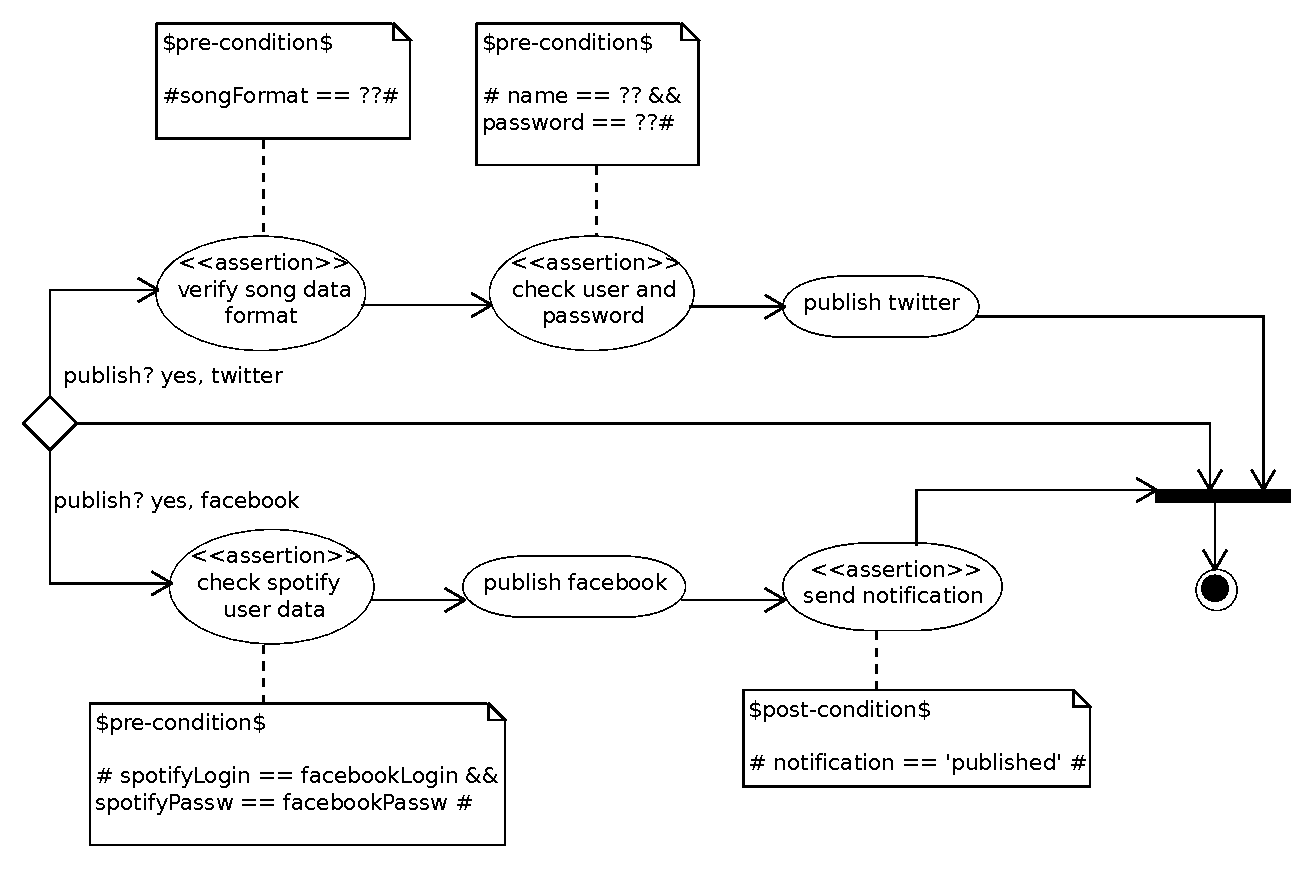
\includegraphics[width=.89\textwidth]{chapters/methodology/figs/piserviceprocess/runningExampleSP_part.pdf}
% \caption{Service Process Model with Contract Definition}
% \label{fig:serviceprocessContractPart}
% \end{figure}



Each {\sc Use Case} modelled in the use case diagram are refined into {\sc
Actions} in the service process diagram. The set of {\sc Constraints} are
transformed into {\sc Assertions} and {\sc Contracts}. The \textit{buy music}
and \textit{publish music} services (update Twitter and Facebook) has pre- and
post-conditions assertions that are composed into a contract for each service. 
 The  \textit{buy music} pre-conditions are: (i) verify if the User
data are correct; (ii) if the User is already logged in Spotify; (iii) if bank
account information are correct and; (iv) if there is enough money to make the
payment. As post-condition, it ensures the complete transaction and verify if a
notification were sent to the user and Spotify, about the payment authorization.
There are four assertions for the \textit{buy music} action, and each assertion
has been detailed with the assertion property and predicate that must be verified. 
To \textit{update} services, depending of each service, there may be different
restrictions. As an example, a new verification of user data and message format
is appropriate (maximum 140 characters), in case of Twitter. In the case of Facebook, it is required that
the user is already logged on Spotify and these data are the same as
Facebook. As post-condition, it ensures that the Facebook service send a
notification of success. To update Twitter a
pre-condition is required, while to update Facebook is necessary
a pre-condition and a confirmation notice is modelled as post-condition. As a
pre-condition for ``\textit{twitter update}'' it is necessary that \textit{(i)}
the music format be correct and (\textit{ii})  the twitter login and password be
correct for the update.


\bigskip 
\bigskip

After modeling of service process, its features, and the
service contracts, it is necessary to model the service composition process and
its policies. $\pi$SOD-M uses a service composition diagram
to describe the third party services and each policy allied to
each composition \correctingText{(as presented in Figure
\ref{fig:developmentProcess})}. In the next section we present this model and their
respective policy concept .
 
\subsection{$\pi$-ServiceComposition Model}

The service composition model represents the workflow needed to execute a
service or a set of them, but in a more detailed way, \textit{i.e.}, identifying
those entities that collaborate with the service process workflow, performing
services that are necessary to execute the actions (in the business
collaborators). Considering the workflow described in the
\textit{$\pi$-ServiceProcess} diagram, this model identifies the services and
functions that correspond to each action in the business process.

Each action describes a fundamental behaviour unit that is part of a service
activity and represents some behaviour in the system being
modelled. The \textit{$\pi$-ServiceComposition} model refines the concepts
described in the \textit{$\pi$-ServiceProcess} model, grouping contracts
into policy (figure \ref{fig:serviceprocess}).

% The main difference between the \textit{service composition} diagram proposed by
% SOD-M \cite{valeriaThesis} and our \textit{$\pi$-ServiceComposition}  model is
% the inclusion of concepts that represent policy and rules related with service
% compositions.


\subsubsection{\textit{$\pi$-ServiceComposition} Diagram, Terms and Concepts} 
  


% \bigskip
%  \textbf{Properties} 
%  \bigskip 
%  
 A \textit{$\pi$-ServiceComposition} model represents service
 compositions and their related business collaborators (external services),
 policies, rules associated with a policy and the whole application
 process and functionalities. 
 
%  What differentiates this model from the
%  \textit{$\pi$-ServiceProcess} model is its particular content and the form of
%  their presentation.
%  
 This model is essential for the organization and modeling of
 services and their location. We refine the representation of packages
 described in the  \textit{$\pi$-UseCase} model into business
 collaborator. The set of use cases described in a package
 (\textit{$\pi$-UseCase} model) will be represented by an external service
 functions.
 
 Figure \ref{fig:businesscollaborator_detail} shows how to relate the actions
 described in the \textit{$\pi$-ServiceProcess} model with services of a specific business
 collaborator. A service is represented by an stereotyped action 
 (\textit{<<service>>}), and their connection is made by an edge (\textit{Object
 Flow}). Thus each action described in the application workflow may be
 replaced by a service or a composition of them. If there is no relationship
 between the actions described in the application workflow (\textit{External
 false} business collaborator) with external services, means that function
 is native to the application being developed.
    
\begin{figure}[ht!] 
\centering
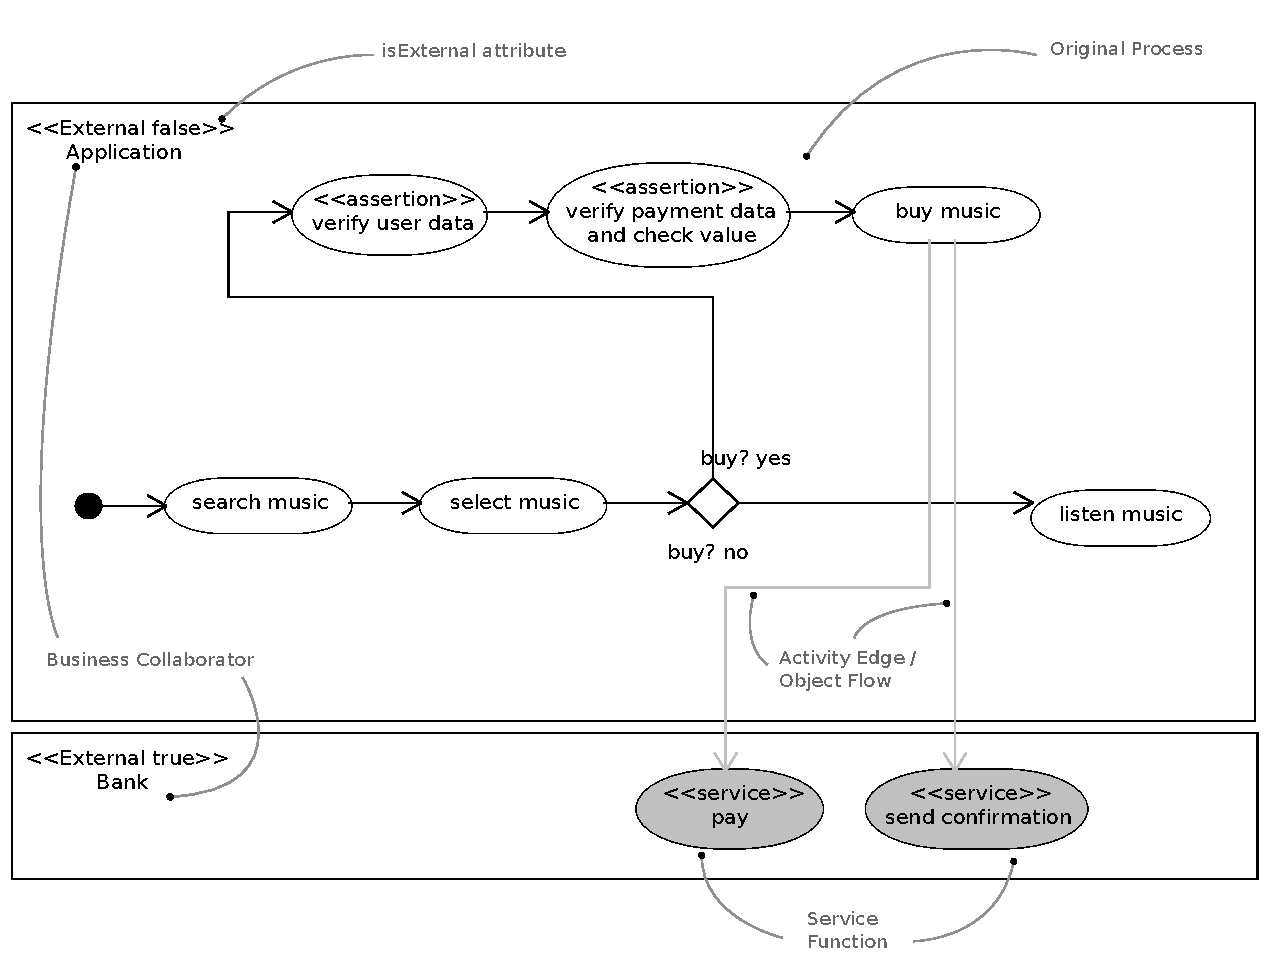
\includegraphics[width=0.99\textwidth]{chapters/methodology/figs/serviceComposition_detail}
\caption{Business Collaborator Representation.}
\label{fig:businesscollaborator_detail}
\end{figure}
  
\begin{figure}[ht!] 
\centering
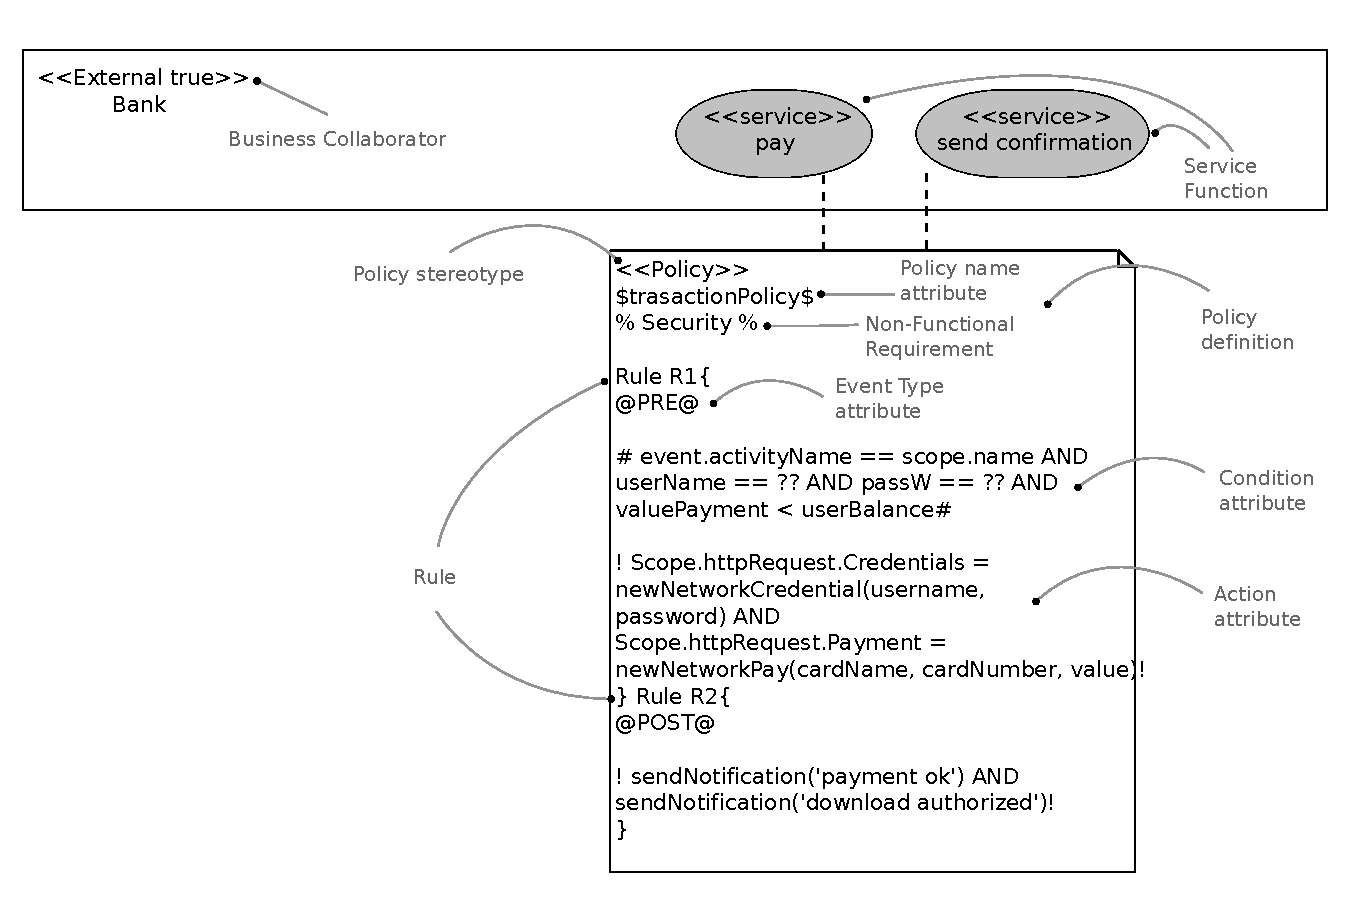
\includegraphics[width=0.99\textwidth]{chapters/methodology/figs/policy_detail}
\caption{Policy Representation.}
\label{fig:policy_detail}
\end{figure} 

The main properties described in the  \textit{$\pi$-ServiceComposition} model
for the ``\textit{to publish music}'' example are: (i) description of workflow
application (\textit{External false}), where the business collaborator \textit{Application} points out that it is not an
external workflow, (ii) the external services (\textit{business collaborators})
and (iii) the application policies. Figures
\ref{fig:businesscollaborator_detail} and \ref{fig:policy_detail} presents how
to model the \textit{$\pi$-ServiceComposition} concepts (figure
\ref{fig:servicecomposition}).

Figure \ref{fig:businesscollaborator_detail} shows how each action is connected to an external service
(through \textit{Activity Edge - Object Flow}), and how to define the
description of each business process, while Figure  \ref{fig:policy_detail} shows each
policy property and how it should be presented in the model. 

Each business collaborator encompasses a set of services that can
be performed by the application. These external services are used by the 
application must be described in this model, and not in the
\textit{$\pi$-ServiceProcess} model. The contracts described for each action are
refined into policies, considering the non-functional requirement of each
contract.



 \subsubsection{Meta-model} 
 
 

Considering the $\pi$SOD-M concepts (figure \ref{fig:pisodm-concepts}), the
\textit{$\pi$-ServiceComposition} meta-model (figure
\ref{fig:servicecomposition}) describes the service compositions
to be modelled and the policies related with each service composition.
The $\pi$SOD-M concepts modelled in the \textit{$\pi$-ServiceComposition}
meta-model are: {\sc Policy, Rule, Variable, Exceptional Behaviour, Service
Activity, Action, Business Collaborator} and {\sc Non-Functional
Requirement}.

 $\pi$SOD-M proposes representing this model using the a extension of UML
 activity diagram technique. This extension describes the relationship of each {\sc Action} for the
respective {\sc Service Activities}. Thus, as shown in figure
\ref{fig:servicecomposition}, the meta-model includes typical modeling elements
of the activity diagram such as {\sc Activity Nodes}, {\sc Initial
Nodes} and {\sc Final Nodes}, {\sc Decision Nodes}, etc., along with
new elements defined by $\pi$SOD-M such as {\sc Business Collaborator},
{\sc Service Activity} and {\sc Action} (see
figures \ref{fig:servicecomposition} and \ref{fig:servicecompositionPolicy}).

All \textit{$\pi$-ServiceComposition} models
describe the set of services and its relation with the service process and its
activities that need to be performed. So, the external services
are represented by the {\sc Business Collaborator} concept. All service
composition may specify a {\sc Policy} as restriction. A {\sc Policy} is the
set of {\sc Contracts} related with the service process expressed in the
previous model (\textit{$\pi$-ServiceProcess}).

 

Policy over service activities and business collaborators are not described in
the original SOD-M method. The rule concept grouped into policy and
exceptional behaviour make possible to model restrictions on service composition. Entities
highlighted in the \textit{$\pi$-ServiceComposition} (figure
\ref{fig:servicecomposition}) meta-model are the difference from the original
SOD-M service composition model.


\begin{figure}[ht!]
\centering
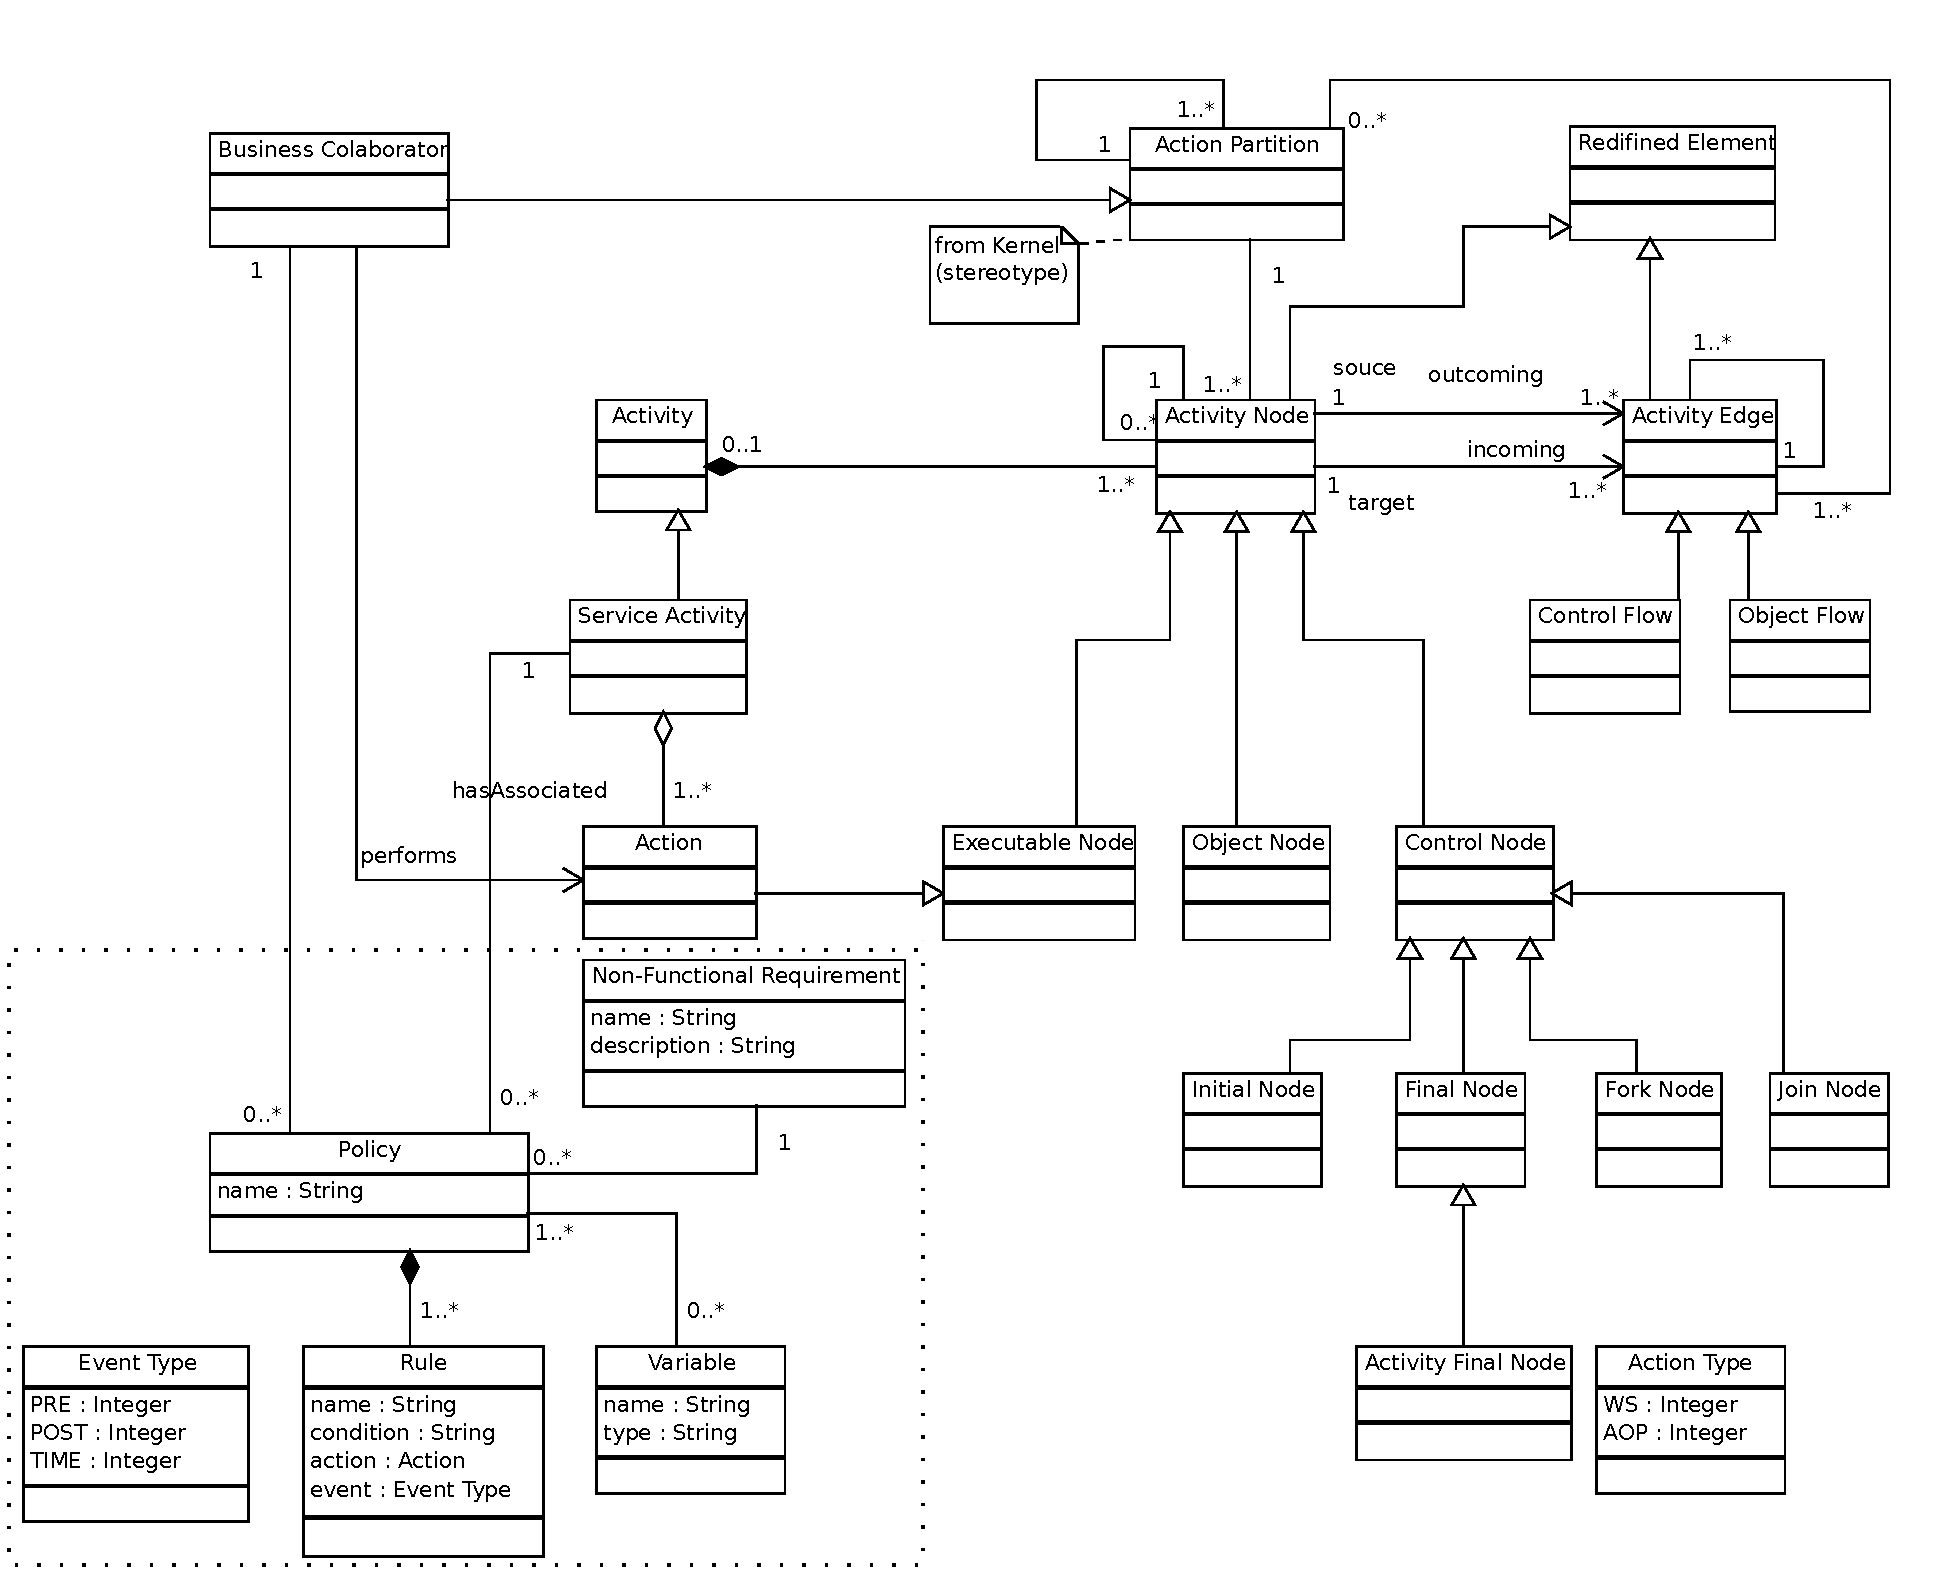
\includegraphics[width=1.0\textwidth]{chapters/methodology/figs/PiServiceComposition}
\caption{\textit{$\pi$-ServiceComposition} Concepts (Meta-model).}
\label{fig:servicecomposition}
\end{figure}

A {\sc Business Collaborator} element represents those
entities that collaborate in the business processes by
performing some of the required actions. They are graphically
presented as a partition in the activity diagram.
A collaborator can be either internal or external to the
system being modelled. When the collaborator of the
business is external to the system, the attribute \textit{IsExternal} of the
collaborator is set to \textit{true}.

{\sc Action}, a kind of {\sc Executable Node}, are represented
in the model as an activity. Each action identified in
the model describes a fundamental behaviour unit which
represents some type of transformation or processing
in the system being modelled. There are two types of
actions: i) a Web Service (attribute Type is \textit{WS}); and ii) a
simple operation that is not supported by a Web Service,
called an {\sc Activity Operation} (attribute Type is \textit{AOP}).

The {\sc Service Activity} element is a composed activity
that must be carried out as part of a business service and
is composed of one or more executable nodes.


The policy based service composition model refines the concept contract of
service process model. A policy assemble a set of contracts and can be
applied to more than one activity. The restriction on service composition model
is marked with the stereotype \texttt{<<policy>>}.


An {\em Policy} groups a set of rules. It describes global variables and
operations that can be shared by the rules and that can be used for expressing
their Event  and Condition parts. An {\em Policy} is associated to the
elements {\sc Business Collaborator}, {\sc Service Activity} and, {\sc Action}  of
the $\pi$-ServiceComposition meta-model (see figure
\ref{fig:servicecomposition}) .

% Instead of programming different protocols within the application logic, we
% propose to include the modeling of non-functional requirements like
% transactional behaviour, security and adaptability at the early stages of the
% services' composition engineering process.



 \subsubsection{UML Concepts Representation} 
 
 
 

The representation described in figure \ref{fig:picomposition_representation}
presents how the user of the methodology's user apply the concepts described in
the \textit{$\pi$-ServiceComposition} meta-model. In the specific case
of \textit{$\pi$-ServiceComposition} meta-model, those concepts will be used to
describe how {\sc Business Collaborator, Action, Service Activity, Policy and
Rules} can be specified. Figure \ref{fig:picomposition_representation}
also describes how the proposed concepts can be modelled in real system
development cases. All \textit{$\pi$-ServiceComposition} based models
(presented in figure \ref{fig:picomposition_representation}) must follow the
meta-model description and its constraints.
 

\begin{figure}[ht!]
  \centering
  \subfloat[\textit{Service Activity} and \textit{Business Collaborator}  Model]
  {\label{fig:pisc1}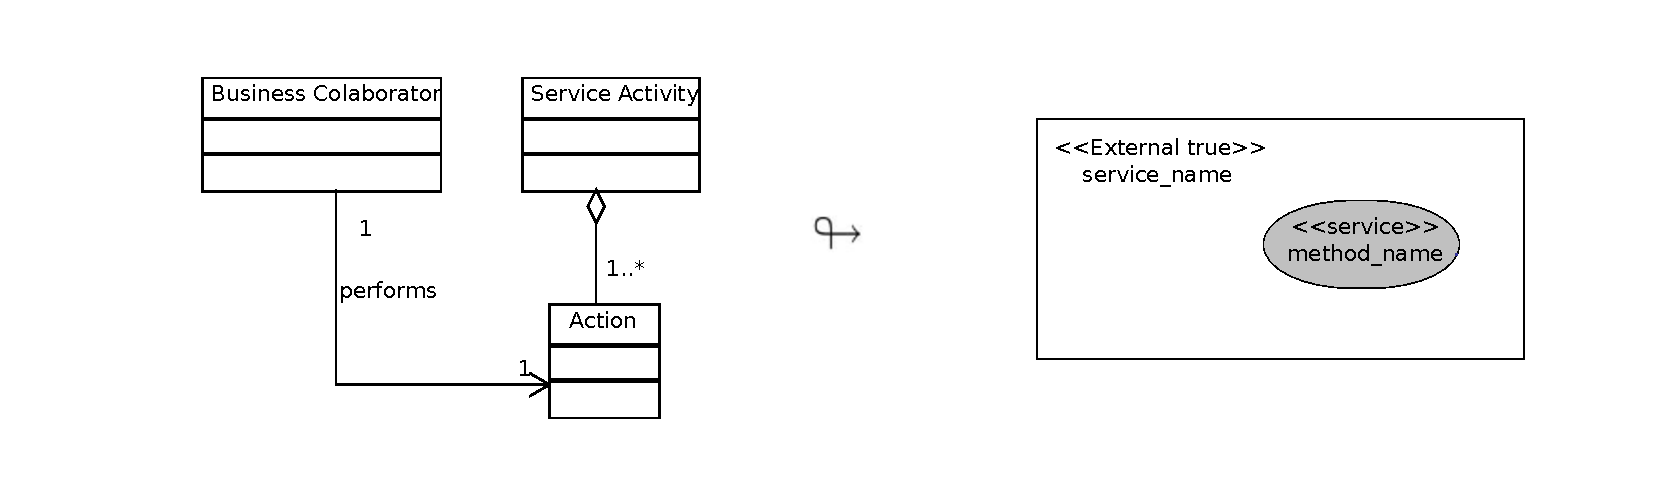
\includegraphics[width=0.8\textwidth]{chapters/methodology/figs/piservicecomposition/serviceComposition1}}
  ~ %add desired spacing between images, e. g. ~, \quad, \qquad etc. (or a blank line to force the subfig onto a new line)
  \\
  \subfloat[\textit{Policy} and \textit{Rule}  Model]
  {\label{fig:pisc2}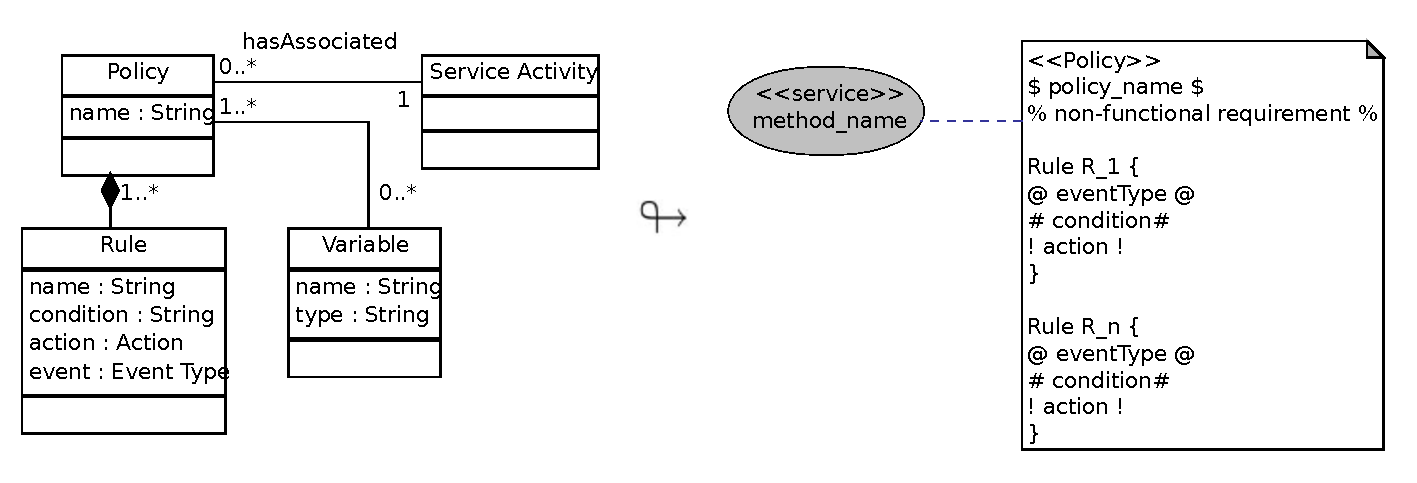
\includegraphics[width=0.8\textwidth]{chapters/methodology/figs/piservicecomposition/serviceComposition3}}
   %add desired spacing between images, e. g. ~, \quad, \qquad etc. (or a blank line to force the subfig onto a new line)
  ~
  \\
  \subfloat[\textit{Business Collaborator - External false} Model]
  {\label{fig:pisc3}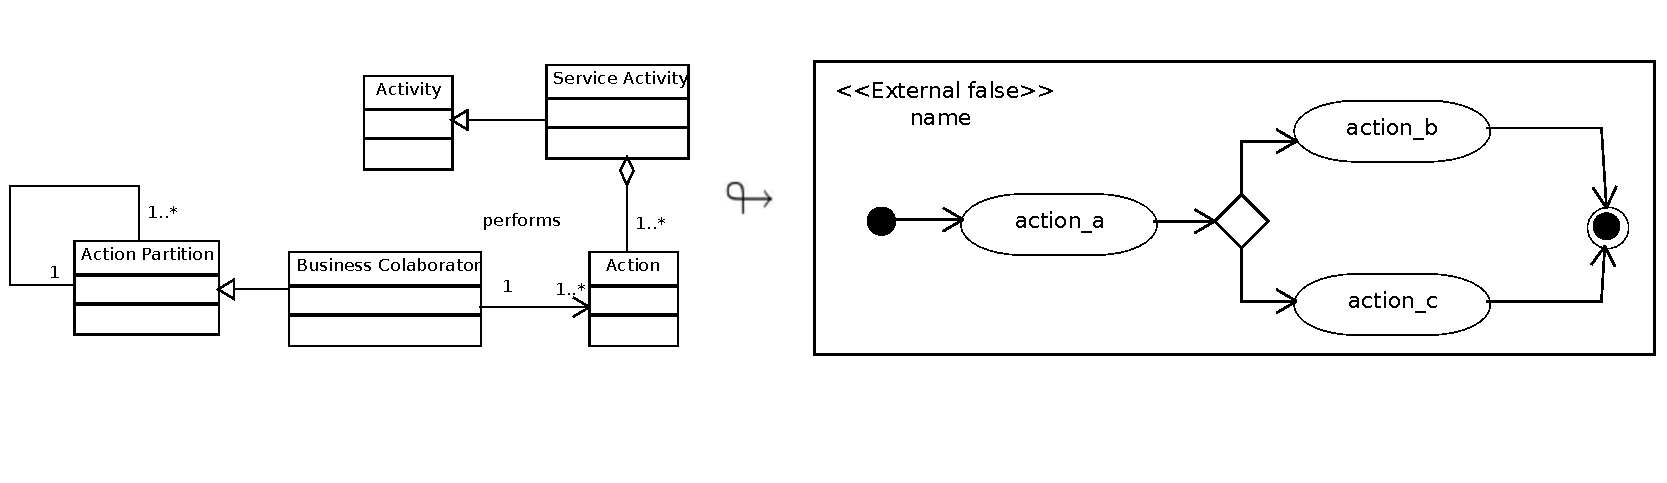
\includegraphics[width=0.8\textwidth]{chapters/methodology/figs/piservicecomposition/serviceComposition2}}
  ~ %add desired spacing between images, e. g. ~, \quad, \qquad etc. (or a blank line to force the subfig onto a new line)
  \\
  \subfloat[\textit{Business Collaborator - External true} Model]
  {\label{fig:pisc4}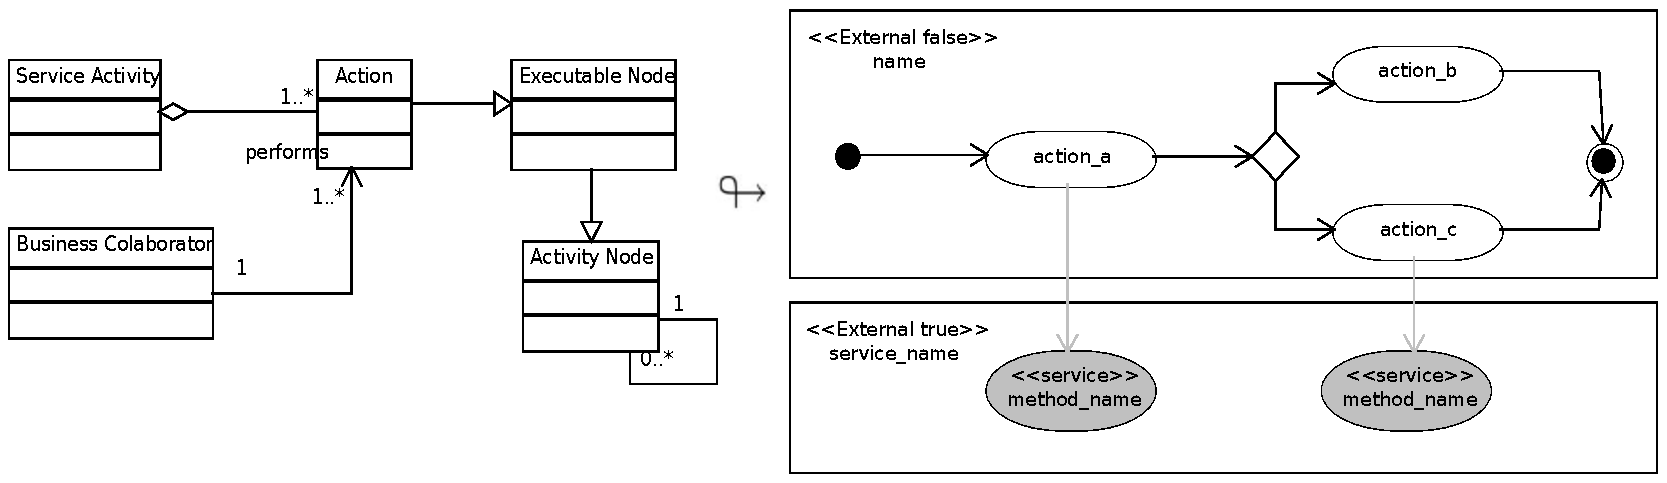
\includegraphics[width=0.8\textwidth]{chapters/methodology/figs/piservicecomposition/serviceComposition4}}
  ~ %add desired spacing between images, e. g. ~, \quad, \qquad etc. (or a blank line to force the subfig onto a new line)
  \caption{\textit{$\pi$-ServiceComposition} Representation Models.}
  \label{fig:picomposition_representation}
\end{figure}

Figure \ref{fig:pisc1} presents the representation for the relation between
{\sc Action} and {\sc Business Collaborator}. As a {\sc Service Activity} are
modelled as a set of {\sc Actions} (service functions), they are represented as
\textit{<<External true>>} {\sc Business Collaborator}. It means that an
external service is invoked by the application's function. Each {\sc Business
Collaborator} can represents an external service. Figure \ref{fig:pisc2}
presents the representation for the relation between {\sc Action}, {\sc Policy} and {\sc
Rule}. Figure \ref{fig:pisc3} presents the representation of the original
\textit{Service Process} associated to the \textit{<<External false>>} {\sc
Business Collaborator} and figure \ref{fig:pisc4} presents how to associate the
\textit{Service Process}' {\sc Action} with real services.

Notice that all \textit{$\pi$ServiceComposition} meta-model concepts can be
represented in the real application model, as we illustrate next using the
scenario example.

\subsubsection{\textit{Publish Music} Service Composition}

To illustrate the use of the \textit{$\pi$-ServiceComposition} model we used it for
defining the policy based composition model of the example scenario (see figure
\ref{fig:servicecompositionPolicy}). There are four external {\sc Business
Collaborators}, they are: \textit{Bank, Spotify, Twitter} and \textit{Facebook}.
The model also shows the business process of the application that consists of
six {\sc Service Activities} (see figure \ref{fig:example_serviceprocess}):
\textit{search music, select music, buy music, download music, listen music} and
\textit{publish music}. Note that the action \textit{publish music} of the
application calls the actions of two service collaborators namely Facebook and
Twitter, and the action \textit{buy music} of the application calls two actions
of the service collaborator Bank.

\begin{figure}[ht!]
\centering
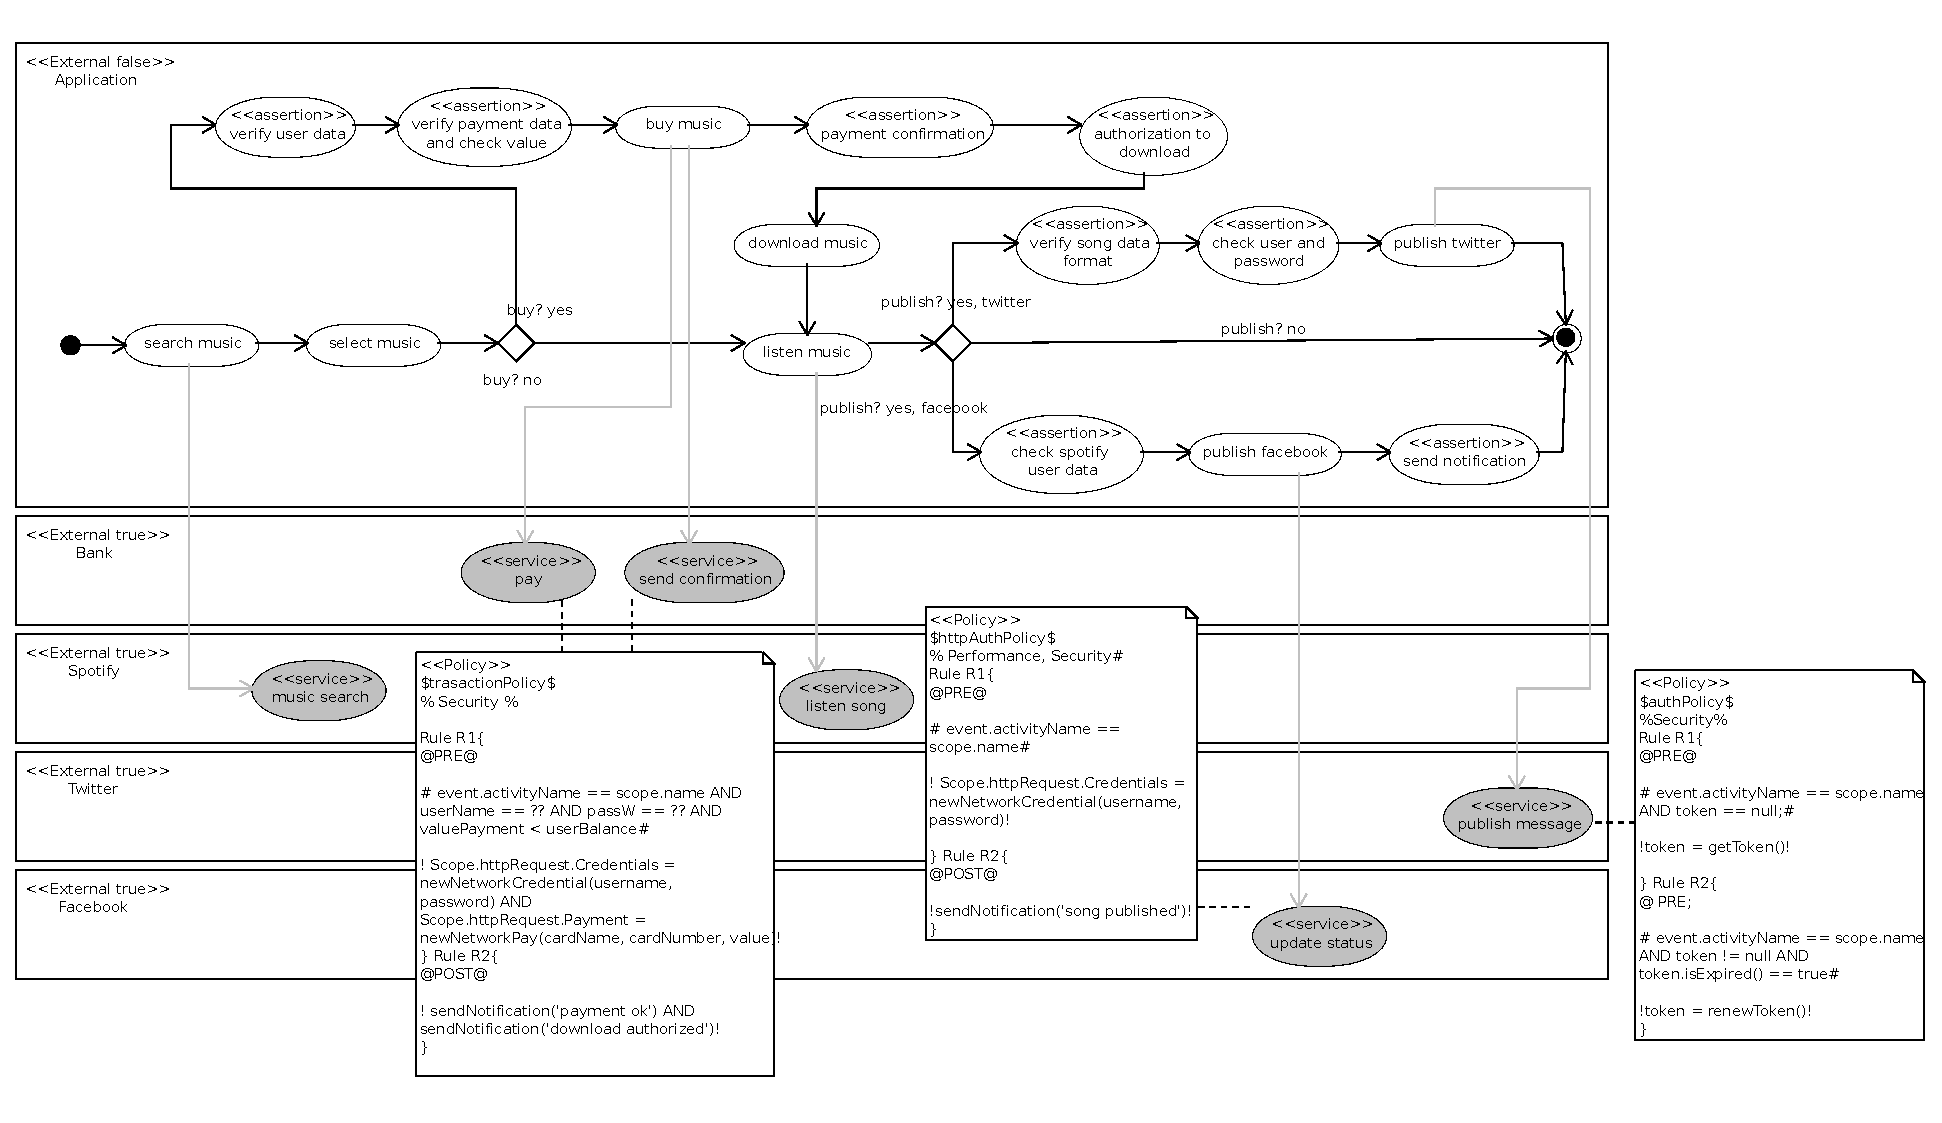
\includegraphics[width=.99\textwidth]{chapters/methodology/figs/runningExampleServiceComposition.pdf}
\caption{Service Composition Model with Policy Definition - Spotify Music
Service.}
\label{fig:servicecompositionPolicy}
\end{figure}


The {\em Facebook} and {\em Twitter} services require authentication
protocols in order to execute methods that will read and update the users'
space. A call to such services must be part of the authentication protocol
required by these services. In this example we  associate two authentication
policies, one for the open authentication protocol, represented by the class
{\sf\small Twitter AuthPolicy} that will be associated to the activity
{\sf\small UpdateTwitter} (see figure \ref{fig:servicecompositionPolicy}). In
the same way, the  class {\sf\small Facebook HTTPAuthPolicy}, for the http
authentication protocol will be associated to the activity {\sf\small
UpdateFacebook}. {\sf\small OAuth}  implements the open authentication protocol.
As shown in figure \ref{fig:servicecompositionPolicy}, the {\em Policy} has a
variable {\sf\small Token} that will be used to store the authentication token
provided by the service. This variable is imported through the library
{\sf\small Auth.Token}. The {\em Policy}  defines two rules, both can be
triggered by events of type {\sf\small ActivityPrepared}: (i) if no token has
been associated to the variable {\sf\small token}, stated in by the condition of
rule {\sf\small R$_1$}, then a token is obtained (action part of {\sf\small
R$_1$}); (ii) if the token has expired, stated in the condition of rule
{\sf\small R$_2$}, then it is renewed (action part of {\sf\small R$_2$}). Note
that the code in the actions profits from the imported  {\sf\small Auth.Token}
for transparently obtaining or renewing a token from a third party.
 
HTTP-Auth implements the HTTP-Auth protocol.  As shown in figure
\ref{fig:servicecompositionPolicy}, the {\em Policy} imports an http protocol
library and it has two variables {\sf\small username} and {\sf\small password}.
The event of type {\sf\small ActivityPrepared} is the triggering event of the
rule {\sf\small R$_1$}. On the notification of an event of that type, a
credential is obtained using the username and password values. The object
storing the credential is associated to the scope, i.e., the activity that will
then use it for executing the method call.

\bigskip
\bigskip

Thanks to rules and policies it is possible to model and associate
non-functional properties to services' compositions  and then generate the code.
For example, the atomic integration of information retrieved from different
social network services, automatic generation of an integrated view of the
operations executed in different social networks or for providing security in
the communication channel when the payment service is called.

Back to the  definition process of a SIS, once the {\em Policy} based services'
composition model has been defined, then it can be transformed into a model
(i.e., $\pi$-PEWS model, Section \ref{sec:psm-pisodm}) that can support then
executable code generation. 

% The following Section describes the $\pi$-PEWS
% meta-model that supports this representation.

\section{$\pi$-PEWS Platform Specific Models}
\label{sec:psm-pisodm}



Platform specific models (PSMs) are used to combine the specifications in
the PIM with the details of the chosen implementation platform. PSM
models are used to implement the system (generating code automatically), and
they must provide all information needed to build the system and its
components. A PSM model can also run as a model to be used for further
refinements by others PSM models.


$\pi$SOD-M platform model proposed at PSM level combines
specific details of the service-based platforms. We use a $\pi$-PEWS language
meta-model for representing the specification of a service composition on the
language. A model can be then used to generate the corresponding code.
$\pi$-PEWS~\cite{Placido2010LTPD} is a extension of the PEWS language that
provides constructs for specifying policies for services through contracts clauses (see Appendix \ref{append:pews_language}).

% From models described in PEWS, the code can be automatically generated. We extend the PEWS language, and named the its extension as
% $\pi$-PEWS (see Appendix \ref{append:pews_language}), and aggregate to it
% constructs for specifying policies for services through contracts clauses.

\subsection{$\pi$-PEWS Specification, Terms and Concepts}

 A \textit{$\pi$-PEWS} model represents the system
 specification. This model is essential for the system specification,
 detailing the services, compositions and system's constraints. A
 \textit{$\pi$-PEWS} specification describes the behavioural aspects of the
 system.
 
 We extended the PEWS language~\cite{Placido2010LTPD} to support the notion
\textit{policy} through contracts definitions (see figure
\ref{fig:contractRepresentation} and appendix \ref{append:pews_language}). The
extension does not modify the syntax of existing PEWS programs, but complements
it by specifying (non-functional) restrictions in a separate block. This feature
is intended to enhance reusability and allows the programmer to adequate a
program to specific requirements of the application being developed. This means
that the program developer can reuse the control part of the program and add
application-specific requirements as contract or time constraints.

 \begin{figure}[ht!]
\centering
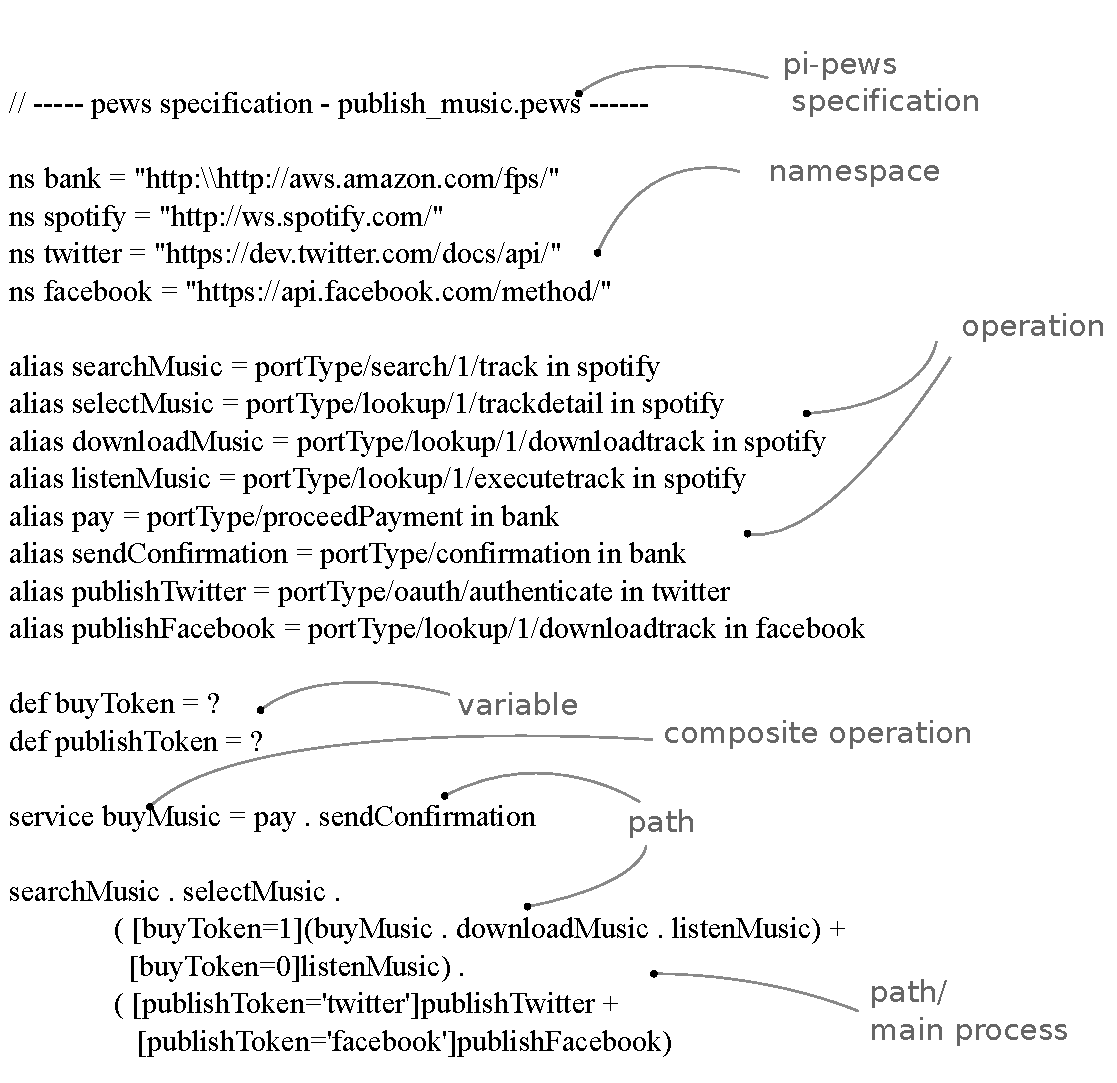
\includegraphics[width=.9\textwidth]{chapters/methodology/figs/pewsEspecification.pdf}
\caption{$\pi$-PEWS Specification Representation.}
\label{fig:pewsRepresentation}
\end{figure}

 Behavioural web service interface languages describe not only the input/output
interface of a web service but also the expected behaviour of its components.
This behaviour can be specified as a workflow, defining the \textit{order} in
which the components of a service will be executed, so that the workflow
specifies the functional behaviour of the compound web service (figures \ref{fig:pewsRepresentation} and
\ref{fig:contractRepresentation}). 

% This is what
% $\pi$-PEWS programs do (figures \ref{fig:pewsRepresentation} and
% \ref{fig:contractRepresentation}).



\begin{figure}[ht!] 
\centering
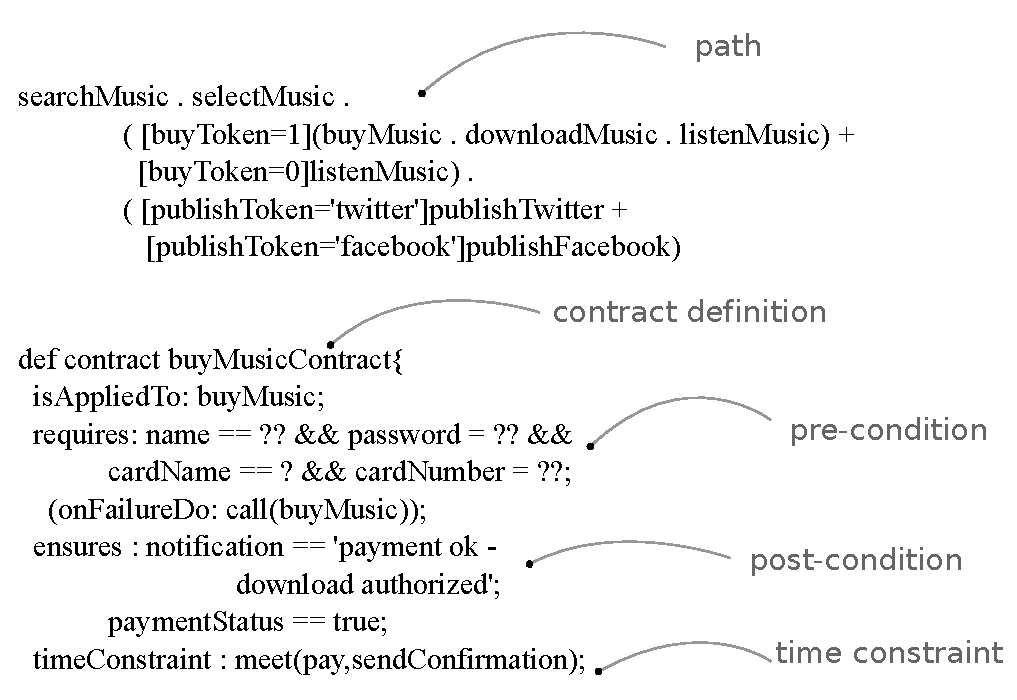
\includegraphics[width=.9\textwidth]{chapters/methodology/figs/pewsEspecificationContract.pdf}
\caption{$\pi$-PEWS Contract Representation.}
\label{fig:contractRepresentation}
\end{figure}

Additionally, we can specify non-functional behaviour for a service;
\textit{i.e}, to impose some additional restrictions which are separated from 
the application's workflow. This can be done by
using the notion of \textit{contract} to be added to each particular instantiation of
the PEWS program. The result of this is to allow a given service (workflow) to
have different restrictions in different contexts.



The policy model proposed here follows the main ideas presented
in~\cite{Espinosa-OviedoVZC09,PortillaHE08}, where contracts are added to a
given composition, as a separate concern. The properties defined by a contract
should be verified at runtime. Recovery actions, defined by the contract, are to
be performed in case of failure of the contract's conditions. Recovery actions
are defined by the contract itself.


\subsection{Meta-model}

% , a programming language that lets the service designer  combine the methods or
% subprograms that implement each operation of a service, in order to achieve the
% desired application logic. 

The idea of the $\pi$-{\sc Pews} meta-model is based on the services'
composition approach provided by the language PEWS
\cite{BHM06,Placido2010LTPD} (\textit{Path Expressions for Web Services}).
Figure \ref{fig:metamodel} presents the $\pi$-{\sc Pews} meta-model consisting of  classes representing:

\begin{itemize}
\item A services' composition: {\sc Namespace} representing the interface exported by a service, {\sc Operation} that represents a call to a service method, {\sc Composite Operation}, and  {\sc Operator} for representing a services' composition and {\sc Path} representing a services' composition.
A {\sc Path} can be an {\sc Operation} or a {\sc Composite Operation}
denoted by an identifier. A {\sc Composite Operation} is defined using an  {\sc Operator}  that can be represent  sequential ($\ . \ $) and parallel ($\ \| \ $) composition of services,
choice ($\ + \ $) among services,
the sequential ($*$) and parallel ($\{\dots\}$) repetition of an operation or the conditional execution of an operation ($[C]S$).

\item {\em Policies} that can be associated to a services' composition:  {\sc A-Policy}, {\sc Rule}, {\sc Event}, {\sc Condition}, {\sc Action}, {\sc State}, and {\sc Scope}.
\end{itemize}
 
\begin{figure}[ht!]
\centering
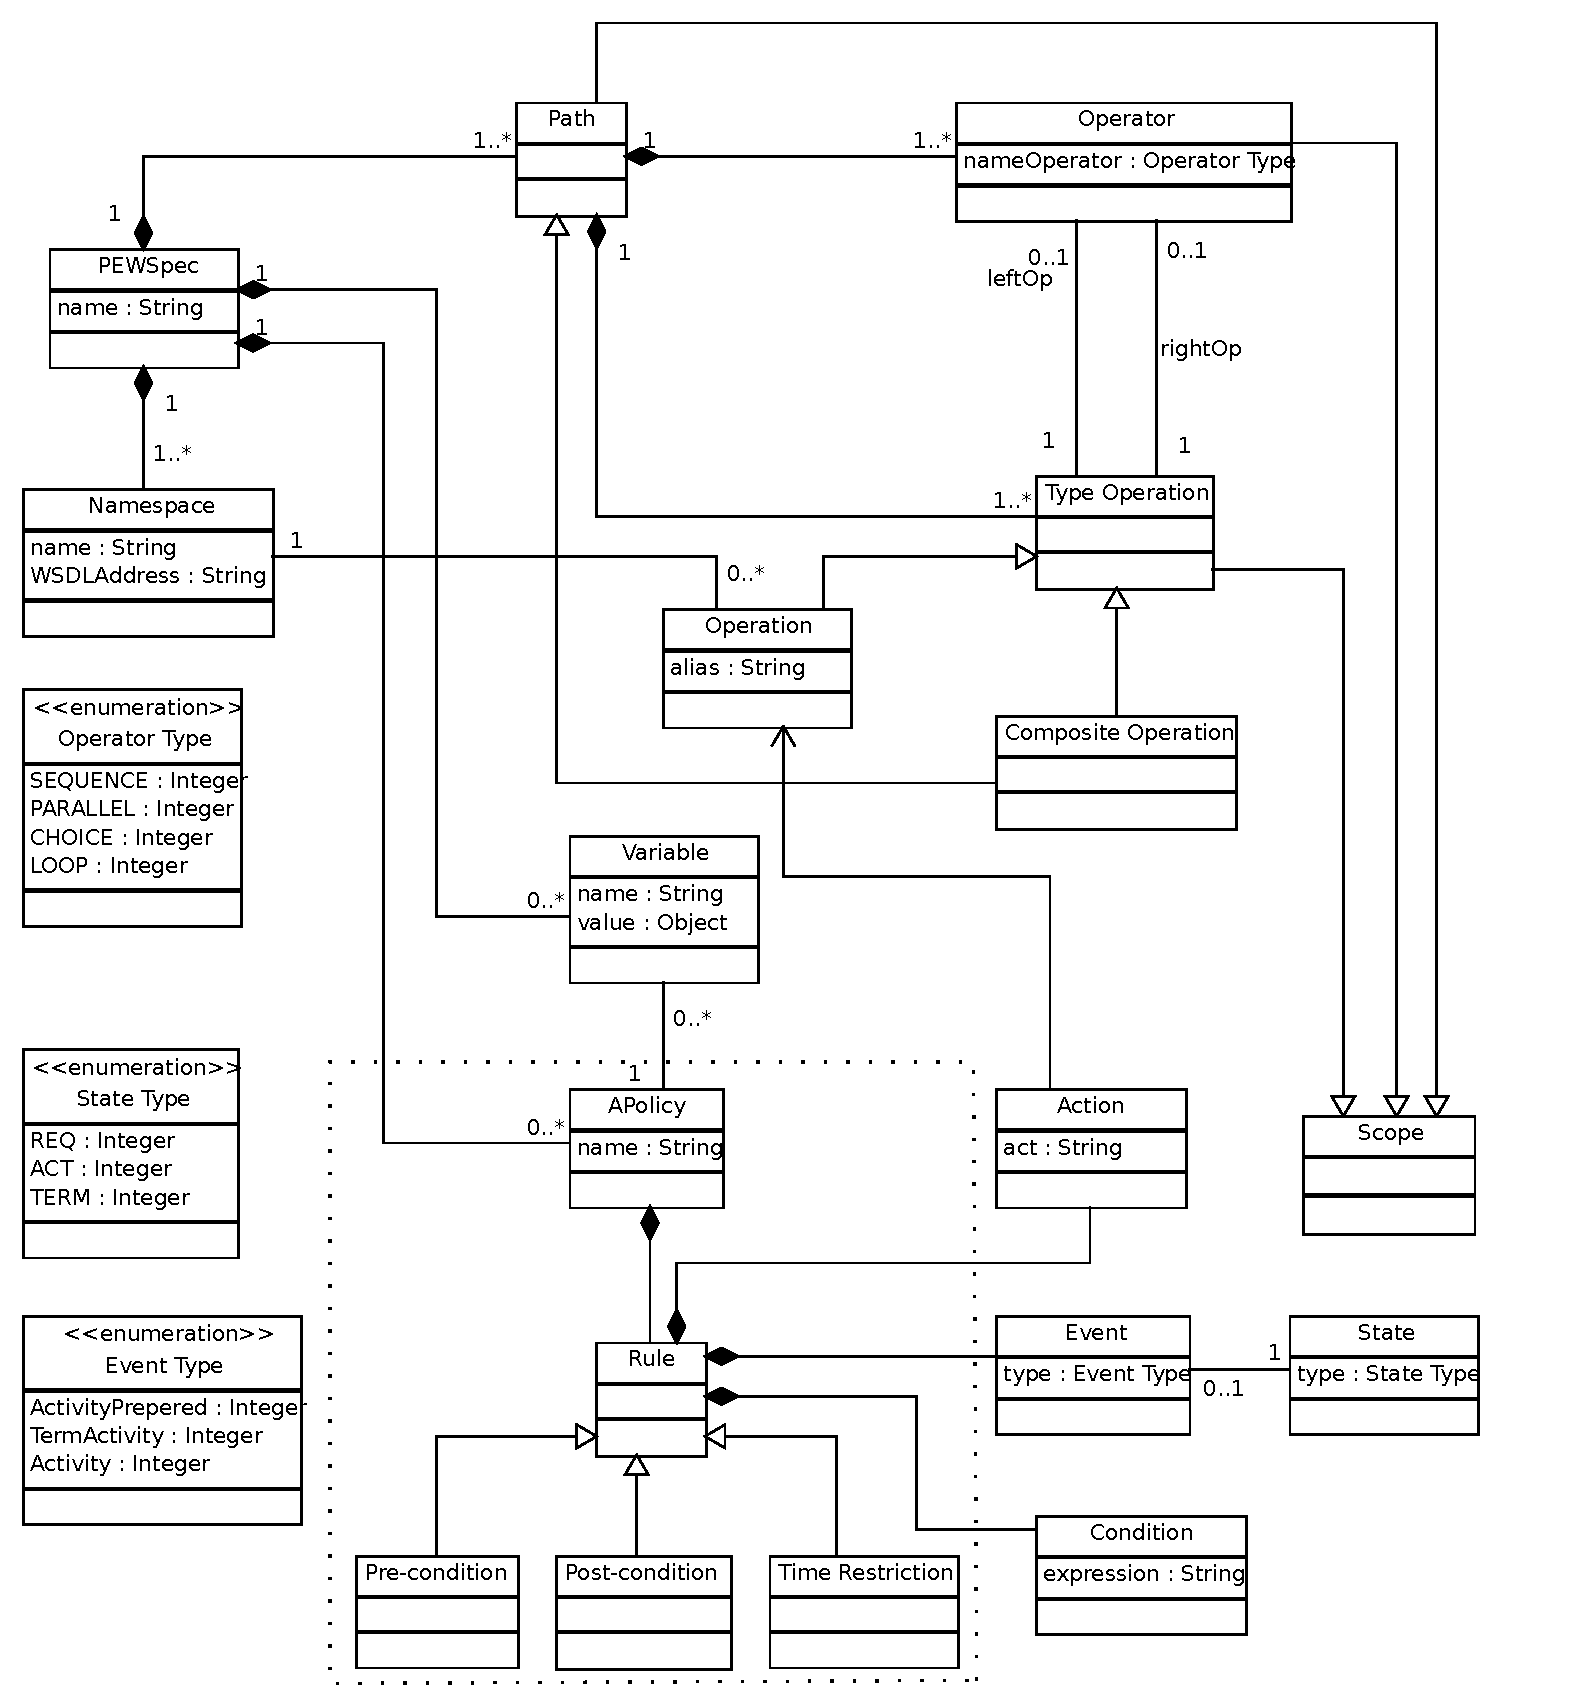
\includegraphics[width=1.0\textwidth]{chapters/methodology/figs/PEWSMetamodel}
\caption{$\pi$-PEWS Meta-model.}
\label{fig:metamodel}
\end{figure}

As shown in the diagram an {\sc Policy} is applied to a {\sc Scope} that can be
either an {\sc Operation} (e.g., an authentication protocol associated to a
method exported by a service),  an {\sc Operator} (e.g., a temporal constraint
associated to a sequence of operators, the authorized delay between reading a
song title in Spotify and updating the walls must be less then 30 seconds), and
a {\sc Path} (e.g., executing the walls' update under a strict atomicity
protocol -- all or noting).  It groups a set of ECA rules, each rule having a
classic semantics, i.e, {\em when an event of type E occurs if  condition C is
verified then execute the action A}.  Thus, an {\em Policy} represents a set of
reactions to be possibly executed if one or several triggering events of its
rules are notified.

\begin{itemize}
\item The class {\sc Scope} represents any element of a services' composition (i.e., operation, operator, path).
\item The class {\sc Policy} represents a recovery strategy implemented by ECA
rules of the form {\sc Event} - {\sc Condition} - {\sc Action}. A {\em Policy}
has variables that represent the view of the execution state of its associated
scope, that is required for executing the rules. The value of a variable is
represented using the type {\sc Variable}. The class {\sc Policy} is specialized
for defining specific constraints, for instance authentication policies.
\end{itemize}

Given a $\pi$-ServiceComposition model of a specific service-based application
(expressed according to the $\pi$-ServiceComposition meta-model), it is possible
to generate its corresponding $\pi$-PEWS model by using transformation
rules. The following Section describes the transformation rules between the
$\pi$-ServiceComposition and $\pi$-PEWS meta-models of our method.

The $\pi$-PEWS language (extension of PEWS) is described in the Appendix
\ref{append:pews_language}. The generated code by $\pi$SOD-M, as end product, is
based on the meta-model shown in figure \ref{fig:servicecomposition} and the
language syntax.
 
% \subsection{\textit{Publish Music} $\pi$-PEWS Specification} 

\section{Model Transformations}
\label{sec:models-tranformation}

A model transformation usually specifies which models are acceptable as input,
and if appropriate what models it may produce as output, by specifying the
meta-model to which model must conform. Model transformations can be seen
as processes that take models as input and produces models as output. There
is a wide variety of kinds of model transformation and uses of them, which differ in their inputs and outputs
and also in the way they are expressed \cite{miller}. A model transformation is
also a way of ensuring that a family of models is consistent, in a precise sense
which the software engineer can define. The aim of using a model transformation
is to save effort and reduce errors by automating the building and modification
of models where possible \cite{atl_manual}.

The $\pi$SOD-M model transformations occur in the two levels, PIM and PSM,
we defined:  PIM-to-PIM and PIM-to-PSM transformations. Transformations in the
same level are considered ``horizontal transformations''. Transformations
between different levels are called ``vertical transformations''. There are 3
model transformations defined in $\pi$SOD-M: $\pi$-UseCase to
$\pi$-ServiceProcess; $\pi$-ServiceProcess to $\pi$-ServiceComposition; and
$\pi$-ServiceComposition to $\pi$-PEWS.

\begin{figure}[ht!]
  \centering
  \subfloat[From one A to one B]
  {\label{fig:rule01}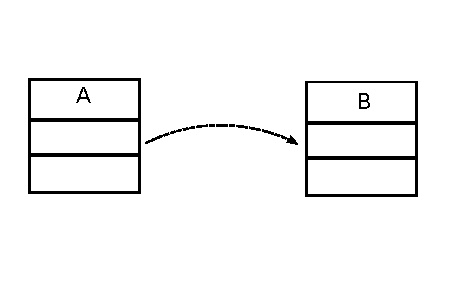
\includegraphics[width=0.33\textwidth]{chapters/implementation/figs/rule01}}
   %add desired spacing between images, e. g. ~, \quad, \qquad etc. (or a blank line to force the subfig onto a new line)
  ~
   \subfloat[From many A to many B]
  {\label{fig:rule02}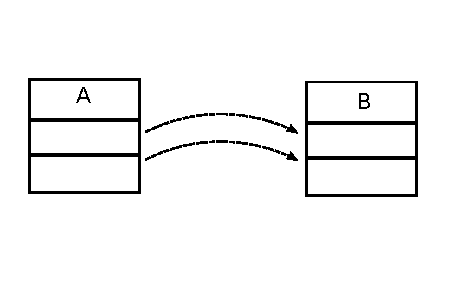
\includegraphics[width=0.33\textwidth]{chapters/implementation/figs/rule02}}
  ~
   \subfloat[From many A to one B]
  {\label{fig:rule03}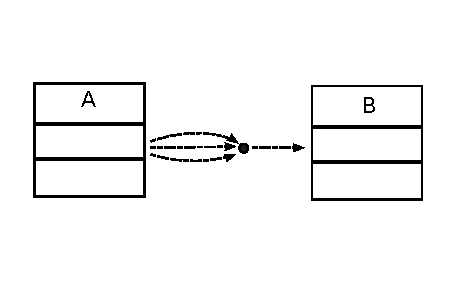
\includegraphics[width=0.33\textwidth]{chapters/implementation/figs/rule06}}
  ~ %add desired spacing between images, e. g. ~, \quad, \qquad etc. (or a blank line to force the subfig onto a new line)
  \\
 \subfloat[From one A to one B, and one C]
  {\label{fig:rule04}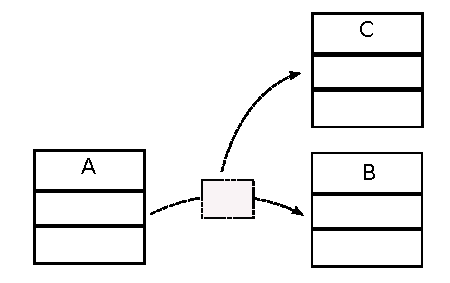
\includegraphics[width=0.33\textwidth]{chapters/implementation/figs/rule03}}
   %add desired spacing between images, e. g. ~, \quad, \qquad etc. (or a blank line to force the subfig onto a new line)
  ~
   \subfloat[From many A to many B, and one C]
  {\label{fig:rule05}\includegraphics[width=0.33\textwidth]{chapters/implementation/figs/rule04}}
  ~
   \subfloat[From many A to many B, and one C]
  {\label{fig:rule06}\includegraphics[width=0.33\textwidth]{chapters/implementation/figs/rule05}}
  ~ %add desired spacing between images, e. g. ~, \quad, \qquad etc. (or a blank line to force the subfig onto a new line)
  \caption{Entities' Model Transformation Rules.}
  \label{fig:rules}
\end{figure}




 All $\pi$SOD-M transformation rules are described in natural language.
 These transformations ensure consistency between the concepts being refined and
 processed at different levels. Figure \ref{fig:rules} presents the set of rules
we defined to apply for each type of transformation. The entities of the
left-hand side represent the source model, and those on the right-hand side
represent the target model. Figure \ref{fig:rule01} shows the transformation
rule in which a single source entity is transformed in a target model entity.
Figure \ref{fig:rule02} describes a many to many entity transformation: a set of
objects from the source model is transformed into a set of objects in the target
model. Figure \ref{fig:rule03} presents a many to one transformation rule: many
objects in the source model it will be transformed into a single object element
in the target model. The next 3 rules are advanced rules, which transform single element in the source model into a set of different elements
in the target model. In figure \ref{fig:rule04}, a source element is
transformed in two different ones, \textit{e.g.} from a ``\textit{A}'' element,
it generates a ``\textit{B}'' and a ``\textit{C}'' element in the target model.
In figure \ref{fig:rule05}, a set of source elements is
transformed into a set of elements ``\textit{B}'' and one ``\textit{C}'' element
in the target model. Finally, figure \ref{fig:rule06} presents the rule which
transforms source elements into a set of elements
``\textit{B}'' and one element ``\textit{C}'' in the target model.

\subsection{From $\pi$-UseCase to
$\pi$-ServiceProcess}

The PIM to PIM transformation process between $\pi$-UseCase and
$\pi$-ServiceProcess (Table \ref{tab:transformationUseCaseToServiceProcess})
models defines how the application requirements are represented as a service
process. At this level, services and general functions are represented as simple
or composite use cases.

Every {\sc Use Case} is transformed into
an {\sc Action} in the \textit{$\pi$-ServiceProcess} model, and every {\sc
Extend} association identified in the \textit{$\pi$-UseCase} model is
transformed into a {\sc Fork Node}, \newText{because several extends relations
implies a conditional verification in the execution workflow}. If the extend
association has only one {\sc Use Case}, the fork will present the {\sc Action} as an alternative flow, and later, both flows will meet. If the extend association has several source
{\sc Use Case}, the fork will present different {\sc Actions} as mutual
alternatives flows, and later, all these flows will meet. A {\sc Activity
Services} (from $\pi$-ServiceProcess meta-model) consists of a composition of
one or more {\sc Actions}. {\sc Action} can be viewed as a method of
the system application. Thus, services are represented as a set of functions in
the \textit{$\pi$-ServiceProcess} meta-model, because {\sc Contracts} modelled
are associated to functions ({\sc Actions}).

All {\sc Constraints} in the source model (\textit{$\pi$-UseCase model}) are
transformed into a {\sc Contract}. A {\sc Contract} is represented as a set of {\sc Constraints}. Each
constrain description is directly transformed into {\sc Assertion}. A set of
{\sc Constraint} of a {\sc Use Case} or a {\sc Composite Use Case} is
transformed into a set of {\sc Assertion} used to define a
{\sc Contract}. All {\sc Use Cases} are associated to a {\sc Non-Functional
Requirement} and all {\sc Constraints} are associated with a {\sc Non-Functional Attribute}. Thus,
{\sc Constraint} representing the same {\sc Use Case} is transformed into a
{\sc Contract}. A {\sc Contract} can have exceptional cases. The negation of the
{\sc Constraint} predicate are treated as {\sc Exceptional Behaviour}. In this
particular case, a {\sc Exceptional Behaviour} will be generated in the target
model. 

The {\sc Constraint Type} can have different transformations, depending of the
following values:

\begin{itemize}
\item If the value of {\sc Constraint Type} is \textit{BUSINESS}, it will be
transformed into none {\sc Assertion};
\item If the value of {\sc Constraint Type} is \textit{VALUE} with the
{\sc Assertion} \textit{isExceptionalBehaviour} attribute setted to
\textit{false}, it will be transformed into one {\sc Assertion};
\item If the value of {\sc Constraint Type} is \textit{VALUE} with the
{\sc Assertion} \textit{isExceptionalBehaviour} attribute setted to
\textit{true}, it will be transformed into a {\sc Exceptional Behaviour};
\end{itemize}

\begin{table}[ht!]
\tiny
\renewcommand{\arraystretch}{1.3}
\caption{Transformation Rules: From $\pi$-UseCase to $\pi$-ServiceProcess.}
\label{tab:transformationUseCaseToServiceProcess}
\centering
\begin{tabular}{l|l|l}
    \hline
    Source  &  Mapping Rules & Target\\
    $\pi$-UseCase meta-model  &   & $\pi$-ServiceProcess meta-model\\
    \hline
    \hline

	Constraint & - All \textbf{Constraints} in the source model will be transformed
	into a \textbf{Assertion} in the target model.  & Assertion, Contract, \\
	 & All \textbf{Use Cases} are associated to a \textbf{Non-Functional
	 Requirement} and all \textbf{Constraints} & Exceptional Behaviour   \\
	 &are associated with a \textbf{Non-Functional Attribute}. Thus,
	 \textbf{Constraint} representing the same Use Case,  &  \\
	& is transformed in a \textbf{Contract}. & \\
	& - A \textbf{Contract} can also have a exceptional cases. The negation of the
	\textbf{Constraint} predicate are treated &\\

	& as the type \textit{EXCEPTIONALBEHAVIOUR}. Thus, all the \textbf{Assertions}
	related to this \textbf{Constraint},  &\\

	&in this particular case, will be transformed in a \textbf{Exceptional
	Behaviour}.&\\
	& - The set of {\sc Assertions} of a {\sc Use Case} are associated with a
	{\sc Contract} & \\
	& - The {\sc Contract} name is formed by ``<useCaseName>'' + ``Contract''
	token. & \\
\hline


	 Constraint Type & - The \textbf{Constraint Type} in source model can have the
	 following transformation: & Assertion\\

	   &  $\bullet$ \textbf{BUSINESS} type is transformed into none
     \textbf{Assertion}; &  Exceptional Behaviour\\

      &  $\bullet$ \textbf{VALUE} with the
     \textbf{Assertion} \textit{isExceptionalBehaviour} attribute setted to false
      is transformed into& \\
     & a \textbf{Assertion} in the target model;&\\

      &  $\bullet$ \textbf{EXCEPTIONALBERAVIOR} with the
      \textbf{Assertion} \textit{isExceptionalBehaviour} attribute setted  & \\
      &to true is transformed into a \textbf{Exceptional Behaviour} in the target
      model.&\\


    & - Both, the  value and exceptional restriction are based on in accordance
    with the values&\\
    & of \textbf{Assertions}&\\

    & - \textbf{Constraint Type} defines the type of restriction on a
    \textbf{Use Case}. &  \\

% \hline
%
% 	Assertion, & Every \textbf{Assertion} associated to an element (\textbf{Assertion
% 	Property} and \textbf{Constraint}) in the source  & Assertion, \\
% 	Assertion Property & model becomes an \textbf{Assertion} associated to the
% 	corresponding element in the target model. & Assertion Property \\
%
\hline

	Non-Functional & Every \textbf{Non-Functional Attribute} associated to an
	element (\textbf{Constraint} and \textbf{Non-Functional} &
	Non-Functional \\ Attribute &  \textbf{Requirements}) in the source model
	becomes a \textbf{Non-Functional Attribute} associated to the  &
	Attribute \\
	&corresponding element (\textbf{Contract}) in the target model. &\\
\hline
    Use Case   &  For every \textbf{Use Case} there will be a
    \textbf{Action} in the service delivery process model & Action  \\
    & describing the Business Service &   \\

    \hline

    Extend (Use Case)    & - Every \textbf{Extend} association identified in the
     \textit{$\pi$-UseCase model} will be represented in the target model   & Control Node, \\
     &by a \textbf{Fork Node}.&  Fork Node,\\
      & - The \textbf{Service Activity} corresponding to the source
      \textbf{ Use Case} of the extend association must be  & Service
      Activity
    \\

      & previous to the \textbf{Service Activity} corresponding to the
      target \textbf{ Use Case} of the extend association. &\\

        &  - If the extend association has only one source \textbf{
        Use Case}, the fork will present the \textbf{Service} & \\
        &\textbf{ Activity} as an alternative to another flow with no \textbf{Service Activity}. Later, both flows will meet;&\\

       &  - If the extend association has several source \textbf{
        Use Case}, the fork will present the different \textbf{Service} & \\
        &\textbf{Activities} as mutual alternatives to another flow with no
        \textbf{Service Activity}. Later, all these flows will&\\
        &meet;&\\
    \hline

      Include (Use Case)    & - An \textbf{Include} association is found in the
      \textit{$\pi$-UseCase model},  the \textbf{Service Activity} corresponding to the    &
      Service Activity \\
       &source must be subsequent to the \textbf{Service Activity} corresponding
       to the target \textbf{ Use Case} of the & \\
      &include association;&\\

        &  - If the include association has several targets, the designer must
        decide the appropriate sequence & \\
        & for the different \textbf{Service Activities} corresponding to the
        target  \textbf{ Use Case} (which will obviously&\\

        &  be previous to the \textbf{Service Activity} corresponding to the
        source \textbf{ Use Case}).&\\

\hline

	Requirement & - A \textbf{Requirement} in the source model is transformed into
	\textbf{Service Activity} of the target model. & Service Activity
	\\ & - The rules for a \textbf{Requirement} to be transformed into a  &\\
	& service activity is analyzed after the transformations of included and
	extended use cases.&\\
	 &- A \textbf{Requirement} associated with only one \textbf{Use Case} in the
	 source model is transformed in a.&\\
	 &\textbf{Service Activity} and an \textbf{Action}, respectively. &\\
	&- All \textbf{Use Cases} must be associated with a \textbf{Requirement}.&\\

\hline

\end{tabular}
\end{table}



\begin{figure}[ht!]
  \centering
  \subfloat[From \textit{Use Case} and \textit{Constraint} to \textit{Action}
  and \textit{Contract}]
  {\label{fig:trans01}\includegraphics[width=0.5\textwidth]{chapters/implementation/figs/trans01}}
   %add desired spacing between images, e. g. ~, \quad, \qquad etc. (or a blank line to force the subfig onto a new line)
   \subfloat[From \textit{Constraint} to \textit{Contract} (2)]
  {\label{fig:trans02}\includegraphics[width=0.5\textwidth]{chapters/implementation/figs/trans06}}
  ~ %add desired spacing between images, e. g. ~, \quad, \qquad etc. (or a blank line to force the subfig onto a new line)
  \\
  \subfloat[From \textit{Composite Use Case} to \textit{Service Activity}]
  {\label{fig:trans03}\includegraphics[width=0.5\textwidth]{chapters/implementation/figs/trans03}}
   %add desired spacing between images, e. g. ~, \quad, \qquad etc. (or a blank
   % line to force the subfig onto a new line)
  \subfloat[From \textit{Requirements} to \textit{Service Activity}]
  {\label{fig:trans04}\includegraphics[width=0.5\textwidth]{chapters/implementation/figs/trans02}}
  \caption{$\pi$-UseCase2$\pi$-ServiceProcess Model Transformation Rules.}
  \label{fig:modelRulesUS2SP}
\end{figure}

Given the \textit{$\pi$-UseCase} model, to all {\sc Constraint} entity related
with a {\sc Use Case}, there is a {\sc Contract} that compounds a set of {\sc
Assertions} entity (figure \ref{fig:trans01}) and the {\sc Use Case} is refined
in a service {\sc Action}.  

\begin{exampl}
Considering the scenario example presented in Section
\ref{sec:example}, the transformation of the ``\textit{listen music}'' {\sc Use
Case} is transformed into a service {\sc Action}. This action is a Spotify
service function that can be invoked to play the music. For ``\textit{publish music}''
{\sc Use Case}, all {\sc Constrains} are transformed in a set of
{\sc Assertions} that are grouped in a {\sc Contract}
(``\textit{publishMusicContract}''). The
``\textit{publishMusicContract}'' is related with the ``\textit{publishMusic}''
{\sc Action}.
\end{exampl}

 
\begin{figure}[ht!]
\centering
\subfloat[From \textit{Extend} to \textit{Fork/Join Flow}]
{\label{fig:trans05}\includegraphics[width=0.9\textwidth]{chapters/implementation/figs/trans04}}
~ %add desired spacing between images, e. g. ~, \quad, \qquad etc. (or a blank line to force the subfig onto a new line)
\\
\subfloat[From \textit{Include} to \textit{Activity Node Flow}]
{\label{fig:trans06}\includegraphics[width=0.9\textwidth]{chapters/implementation/figs/trans05}}
~ %add desired spacing between images, e. g. ~, \quad, \qquad etc. (or a blank line to force the subfig onto a new line)
\caption{$\pi$-UseCase2$\pi$-ServiceProcess Model Transformation Rules (2).}
\label{fig:modelRulesUS2SP2}
\end{figure}

A {\sc Constrain} transformation means that from {\sc Constraint} and {\sc
Constraint Type} entities are generated detailed {\sc Contract} information,
that are refined into {\sc Exceptional Behaviours} and {\sc Assertions} entities
(figure \ref{fig:trans02}). {\sc Constraint} is related with a {\sc Constraint Type}, and there are
different cases for the transformation of this concept. A \textit{Business}
type are transformed into an {\sc Assertion} that does not consider value
attributes information like \textit{maxValue} and \textit{minValue} (see figure \ref{fig:usecasemodel}). These {\sc Assertion} information
attributes are considered if the {\sc Constraint Type} is a \textit{Value}
type. This is semi-automatic, because there is not enough
information in a $\pi$-UseCase model to run a complete automatic transformation.
If the {\sc Constraint Type} is a \textit{Value} type, the designer must specify
the variable information, and its boundary values after the transformation. For this, the designer must consider the {\sc Constraint} and {\sc Use
Case} descriptions. By default, \textit{value constraints} are transformed into
\textit{pre-conditions} and  \textit{business constraints} are transformed into
\textit{post-conditions}. This rule may be adjusted by the designer at the time
of transformation.

A {\sc Service Activity} and the {\sc Actions} are generated from two different
elements in the source model ($\pi$-UseCase), from a {\sc Requirement} or a {\sc
Composite Use Case}. Figures \ref{fig:trans03} and \ref{fig:trans04} present
the transformation schema for {\sc Requirement} and {\sc
Composite Use Case} concepts. Both elements are related with many {\sc Use
Cases} that are transformed in many {\sc Actions}. A {\sc Use Case} are related
with, either, a {\sc Requirement} and a {\sc Composite Use Case}. {\sc Actions}
are related with a {\sc Service Activity}. 

\begin{exampl}
For the execution of the ``\textit{download music}'' use case is necessary
process with the payment process. Thus, the set of {\sc Use Cases} that include the ``\textit{download
music}'' process are transformed in {\sc Actions}, and a {\sc Service Activity}
that aggregates all these {\sc Actions} is also generated. 
\end{exampl}


\begin{figure} [ht!]
\centering

\subfloat[Extended Use Case Example]
{\label{fig:extend01}\includegraphics[width=0.3\textwidth]{chapters/implementation/figs/ucExtended}}
~ %add desired spacing between images, e. g. ~, \quad, \qquad etc. (or a blank line to force the subfig onto a new line)
\subfloat[Extended Use Case Example (2)]
{\label{fig:extend02}\includegraphics[width=0.3\textwidth]{chapters/implementation/figs/ucExtended2}}
\\
\subfloat[Equivalent Service Process Workflow]
{\label{fig:servProc01}\includegraphics[width=0.3\textwidth]{chapters/implementation/figs/servProc}}
~ %add desired spacing between images, e. g. ~, \quad, \qquad etc. (or a blank line to force the subfig onto a new line)
\subfloat[Equivalent Service Process Workflow (2)]
{\label{fig:servProc02}\includegraphics[width=0.3\textwidth]{chapters/implementation/figs/servProc2}}

\caption{Extended Transformation Examples.}
\label{fig:modelRulesUS2SP}
\end{figure}


The transformations for {\sc Extend} and {\sc Include} dependence elements are
not as simple as the previous transformations (figures \ref{fig:trans05}.
The workflow generated for each \textit{<<extends>>} relationship with just two
use cases (figure \ref{fig:extend01}) is described by figure
\ref{fig:servProc01}. The generated workflow contains: one {\sc Fork Node},
one {\sc Join Node}, and four {\sc Control Flow} elements, and also two {\sc
Action} elements, one for each {\sc Use Case}, if there are less than 2 extended
{\sc Use Case}. When there is more than one  \textit{<<extends>>} relationship
among different use cases (figures \ref{fig:extend02} and
\ref{fig:servProc02}), the transformation is proceed as: adding two more {\sc
Control Flow} for each new {\sc Use Case}, and one {\sc Action} for each new
extended {\sc Use Case}.

\begin{exampl}
Considering the scenario example, it is possible to apply
the same rule for the ``\textit{publish music}'' use case, which has two
extended use cases, ``\textit{public twitter}'' and ``\textit{public
Facebook}'', applying the illustration expressed in figures \ref{fig:extend02}
and \ref{fig:servProc02}.  
\end{exampl}

For the {\sc Include} use case elements, the transformation is represented as a
{\sc Action} sequence, as shown in figure \ref{fig:trans06}. For each {\sc Use
Case} element an {\sc Action} element  is generated. For a set of \textit{n}
{\sc Use Cases} we generate \textit{n-1} {\sc Object Flow} elements. Each
{\sc Control Flow} links two {\sc Actions}. 


\begin{exampl}
Given the ``\textit{download music}'' use case from the scenario example, it
includes payment process to buy the music. It is represented as a include in the $\pi$-UseCase model and is
transformed in a sequence flow in the $\pi$-ServiceProcess model (as presented
in figure \ref{fig:include}).
\end{exampl}
  

All this transformation rules from \textit{$\pi$-UseCase} model to
\textit{$\pi$-ServiceProcess} model were validated with the scenario example.
All transformations described in this section are completely automatic, however
information about values and its boundaries are inserted by the designer after
the transformation process.


\begin{figure}[ht!]
\centering
\includegraphics[width=0.5\textwidth]{chapters/methodology/figs/include.pdf}
\caption{Include Transformation Example.}
\label{fig:include}
\end{figure}

\subsection{From $\pi$-ServiceProcess to
$\pi$-ServiceComposition}

The PIM to PIM transformation process from \textit{$\pi$-ServiceProcess} to
\textit{$\pi$-ServiceComposition} model will refine further the application
design. The main goal of this transformation is to group all {\sc Contracts} and
{\sc Actions} in {\sc Policies} and {\sc Service Activities}, respectively. 


All {\sc Actions} entities in the source model will be transformed into an {\sc
Action} in the target model, and every {\sc Service Activity} in the source
model will be transformed into a {\sc Service Activity} in the target model.
This happens because \textit{$\pi$-ServiceComposition} is an extension of
\textit{$\pi$-ServiceProcess}.


For the non-functional specifications, the {\sc Contract} entity with the same
{\sc Non-Functional Requirement} in the source model
(\textit{$\pi$-ServiceProcess} model) will be transformed into a {\sc Policy} in
the target model ($\pi$-ServiceComposition model).  Each {\sc Assertion} will be
transformed into a {\sc Rule:condition} attribute in the target model, but if
the {\sc Assertion} has a value type, the \textit{name}
and the attributes in the source model will be transformed into a
\textsc{Variable} in the target model. The other {\sc Assertion
Property} values remains unchanged.



The {\sc  Assertion:aProperty} attribute can have different transformations,
depending of the following values:

\begin{itemize}
\item \textit{POST-CONDITIONS} are transformed into \textit{POST} in
the $\pi$-ServiceComposition model;
\item \textit{PRECONDITIONS} are transformed into \textit{PRE}
in the $\pi$-ServiceComposition model;
\item \textit{TIMERESTRICTIONS} are transformed into \textit{TIME}
in the $\pi$-ServiceComposition model.
\end{itemize}

The {\sc Exceptional Behaviour} entities will be
transformed into an {\sc Action} in the \textit{$\pi$-ServiceComposition} model,
and every {\sc Non-Functional Attribute} associated to an element
({\sc Contract} and {\sc Non-Functional Requirement}) in the
$\pi$-ServiceProcess model becomes a \textsc{Non-Functional Attribute}
associated to the corresponding element ({\sc Policy}) in the \textit{$\pi$-ServiceComposition}
model.

Table \ref{tab:transformationServiceProcessToComposition} describes the
transformations between \textit{$\pi$-ServiceProcess} and
\textit{$\pi$-ServiceComposition} meta-models.

\begin{table} [ht!]
\tiny
\renewcommand{\arraystretch}{1.3}
\caption{Transformation Rules: From $\pi$-ServiceProcess to
$\pi$-ServiceComposition.}
\label{tab:transformationServiceProcessToComposition}
\centering
\begin{tabular}{l|l|l}
    \hline
    Source  &  Mapping Rules & Target\\
    $\pi$-ServiceProcess meta-model &   & $\pi$-ServiceComposition\\
      &&  meta-model\\
    \hline
    \hline

   Action & All \textbf{Actions} in the source model will be
   transformed in a \textbf{Action} in the target model. &Action\\
   \hline
   Service Activity&  - All \textbf{Service Activity} in the source model will
   be transformed in a \textbf{Service Activity} in the target model. &Service Activity,\\
   \hline
   Contract, & All \textbf{Contract} with the same \textbf{Non-Functional
   Requirement}, in the source model, will be transformed in& Policy\\
   Non-Functional Attribute&  a \textbf{Policy} in the target
   model.&\\
   \hline
   Assertion & Each \textbf{Assertion} will be transformed in a
   \textbf{Rule:condition} attribute in the target model. & Rule:condition\\
   \hline

   Assertion:name, & If the \textbf{Assertion} has the type equal to
   \textit{VALUE}, the \textit{name} and the \textit{type} attribute in the source
   model will & Variable\\
   Assertion:type & be transformed in a \textbf{Variable} in the target model.&
   \\
   \hline
   Exceptional Behaviour & An \textbf{Exceptional Behaviour} and its attributes in
   the source model will be transformed & Rule:action\\
   &in a \textbf{Rule:action} in the target model. &\\
   \hline
   Assertion:aProperty &- Depending on the \textbf{assertion Property} type in
   the source model, it will be transformed in a \textbf{Rule:event}&
   Rule:Event,\\ & in the target model. The transformation rules
    are:& Event Type\\
    &$\bullet$ \textit{PRECONDITION} type is transformed into \textit{PRE}
    in the target model;&\\
    &$\bullet$ \textit{POST-CONDITION} type is transformed into \textit{POST} in
    the target model;&\\
    &$\bullet$ \textit{TIMERESTRICTION} type is transformed into \textit{TIME}
    in the target model.&\\
   \hline

	Non-Functional & Every \textbf{Non-Functional Attribute} associated to an
	element (\textbf{Contract} and \textbf{Non-Functional} &
	Non-Functional \\ Attribute &  \textbf{Requirements}) in the source model
	becomes a \textbf{Non-Functional Attribute} associated to the  &
	Attribute \\
	&corresponding element (\textbf{Policy}) in the target model. &\\
	\hline
\end{tabular}
\end{table}




\begin{figure} [ht!]
  \centering
  \subfloat[From \textit{Contract} and \textit{Assertion} to \textit{Policy}
  and \textit{Rule}]
  {\label{fig:trans07}\includegraphics[width=0.5\textwidth]{chapters/implementation/figs/trans07}}
   %add desired spacing between images, e. g. ~, \quad, \qquad etc. (or a blank line to force the subfig onto a new line)
   \subfloat[From \textit{Action} to \textit{Service Activity} (2)]
  {\label{fig:trans08}\includegraphics[width=0.5\textwidth]{chapters/implementation/figs/trans08}}
  ~ %add desired spacing between images, e. g. ~, \quad, \qquad etc. (or a blank line to force the subfig onto a new line)
  \\
  \subfloat[From \textit{Exceptional Behaviour} to \textit{Action}]
  {\label{fig:trans09}\includegraphics[width=0.6\textwidth]{chapters/implementation/figs/trans09}}
  \caption{$\pi$-ServiceProcess2$\pi$-ServiceComposition Model Transformation
  Rules.}
  \label{fig:modelRulesSp2SC}
\end{figure}


Figure \ref{fig:modelRulesSp2SC} presents the main transformation rules for
this level. The main feature of this
transformation is the generation of a \textsc{Policy} from of a set of {\sc
Contracts}. But, \textit{what is the adopted criterion for this transformation?} The main criteria is that all
{\sc Contracts} from the same {\sc Non-Functional Requirement} will be
transformed in one {\sc Policy}. Thus, we can have {\sc Policies} on:
\textit{Safety, Performance, Reliability}, and so on.

% A set of {\sc Assertions} are composed in one {\sc
% Policy}, transformed directly into {\sc Rules}, and many {\sc Contracts} turn
% into one {\sc Policy}. This happens because all {\sc Assertions} that represent
% a contract, become directly in {\sc Rules}. 

Each \textsc{Assertion} of a\textsc{Contract} ( \textit{$\pi$-UseCase}
model) is transformed into a \textsc{Rule} in the \textit{$\pi$-ServiceProcess}
model. The set of {\sc Constracts} generates a {\sc Policy} composed by those
{\sc Rules}. Thus, the set of {\sc Rules} make up
a single {\sc Policy}. It is important to highlight that only the {\sc
Contracts} of the same {\sc Non-Functional Requirement} is transformed into the
same {\sc Policy}. Different NFRs' {\sc Contracts}, are transformed into
different {\sc Policies}. Figure \ref{fig:trans07} show how this transformation
is made.

Similar to the transformation between {\sc Contract} and
{\sc Policy}, a set of {\sc Actions} is transformed into a single {\sc Service
Activity} entity. {\sc Actions} are related with {\sc Business Collaborator},
and all information related to a {\sc Business Collaborator} are transformed
from {\sc Packages} information ($\pi$-UseCase model). All {\sc Packages}
are transformed into {\sc Business Collaborator}. Figure \ref{fig:trans08}
presents the transformation between {\sc Action} and {\sc Service Activity}
elements.

An exceptional behaviour is triggered by a failure in the verification of the
condition of a rule. An {\sc Exceptional Behaviour}
is performed to preserve the state of the application. Figure
\ref{fig:trans09} presents how an {\sc Exceptional Behaviour} that can be
transformed into an {\sc Action} call.

As the \textit{$\pi$-ServiceComposition} model refines the
\textit{$\pi$-ServiceProcess} concepts at PIM level, a service
previously defined as actions (source model) is refined as composition of
those actions (target model) that are necessary to represent a business
service, identifying who are the partners involved in the realization ({\sc
Business Collaborators}). In addition, $\pi$SOD-M defines a platform specific
model based on web services composition. This model is explicitly
indicates those actions which are (or will be, if not yet implemented) supported
by web services. 

\begin{exampl}
Considering the scenario example, the {\sc
Action}'s \textit{update music} {\sc Contract} is transformed is a {\sc Policy}
with its {\sc Rules}. All contract {\sc Assertions} are transformed in {\sc
Rule} and its attributes, \textit{e.g.} the login and password verification.  The
``\textit{securityLoginPolicy}'' is all set of {\sc Rules} that were transformed
from the {\sc Assertions} in $\pi$-ServiceProcess model. The {\sc Non-Functional
Requirement} information will be used to the {\sc Policy} generation comes from
the initial use case model. Also the {\sc Business Collaborator}
\textit{Facebook} and \textit{Spotify} information came from {\sc Package}
$\pi$-UseCase entity element. All {\sc Contracts} of the same {\sc
Non-Functional Requirement} are composed in a {\sc Policy}.
\end{exampl}


%%%%%%%%%%%%%%%%%%%%%%%%%%%%%%%%%%%%%%%%%%%%%%%%%%%%%%%%%%%%%%
%%%%%% FROM --> SERVICE COMPOSITION; TO PEWS
%%%%%%%%%%%%%%%%%%%%%%%%%%%%%%%%%%%%%%%%%%%%%%%%%%%%%%%%%%%%%% 

\subsection{From $\pi$-ServiceComposition to
$\pi$-PEWS}


Table \ref{tab:transformationServiceCompositionToPEWS} describes the PIM to PSM
transformations between $\pi$-ServiceComposition and $\pi$-PEWS meta-models. We
propose two groups of rules: those that transform services composition
elements of the $\pi$-ServiceComposition into $\pi$-PEWS meta-model elements;
and those that transform rules grouped by policies into A-policy types.

A named action of the $\pi$-ServiceComposition represented by  {\sc\em Action}
and {\sc\em Action:name} is transformed to a  named class {\sc Operation} with a
corresponding attribute name {\sc Operation:name}. A  named service activity
represented by the elements {\sc\em Service Activity}  and  {\sc\em
Service Activity:name} of the $\pi$-ServiceComposition, are  transformed into a
named operation of the $\pi$-{\sc Pews} represented by the elements  {\sc
Composite Operation} and {\sc Composite Operation:name}. When more than one action
is called, according to the following  composition patterns expressed using the
operators {\sc\em merge, decision, fork and join} in the $\pi$-ServiceComposition
the corresponding transformations, according to the PEWS operators presented
above, are:
\begin{itemize}
\item   $op_1 . op_2$ if no {\sc\em Control Node} is specified
\item ($op_1 \parallel op_2) . op_3$ if control nodes of type {\sc\em fork, join} are combined
\item ($op_1 + op_2) . op_3$ if control nodes of type {\sc\em decision, merge} are combined
\end{itemize}

The {\em A-policies} defined for the elements of the $\pi$-ServiceComposition are
transformed into {\sc A-Policy} classes, named according to the names expressed
in the source model. The transformation of the rules expressed in the
$\pi$-ServiceComposition is guided by the event types associated to these rules.
The variables associated to an {\em A-policy} expressed in the
$\pi$-ServiceComposition as {\sc\em $<$Variable:name, Variable:type$>$} are
transformed into elements of type {\sc Variable} with attributes {\sc name} and
{\sc type} directly specified from the elements {\sc\em  Variable:name} and
{\sc\em Variable:type} of the $\pi$-ServiceComposition model.


\begin{table}[ht!]
\tiny
\renewcommand{\arraystretch}{1.3}
\caption{Transformation Rules: From $\pi$-ServiceComposition to $\pi$-PEWS.}
\label{tab:transformationServiceCompositionToPEWS}
\centering
\begin{tabular}{l|l|l}
    \hline
    Source  &  Mapping Rules & Target\\
    $\pi$-ServiceComposition meta-model  &   & $\pi$-PEWS meta-model\\
    \hline
    \hline

    Action   &  - An \textit{Action} in the source model corresponding to an
    external \textbf{Business Collaborator} is mapped  & Operation:alias\\
       &   to an Operation in target model.   & \\
       &   - The \textbf{Action:name} in the source model is transformed into
       \textbf{Operation:name} in the target model.  & \\
    \hline

    Service Activity    & - The \textbf{Service Activity} in the source model is
    mapped to a \textbf{Composite Operation} in target  & Type Operation,\\
        &  model when more than one \textbf{Actions} are called.   &
        Composition Operation\\

        & - If \textbf{Composite Operation} is generated for a given
        \textit{Service Activity} then the \textbf{Service Activity:name} & \\
        & in the source model is mapped to
        \textbf{Composition Operation:name} in the target model. &\\
    \hline

    Control Nodes   &  - The \textbf{Control Node} in the source model is mapped
    to a \textbf{Operator} in target model. According to the & Operator\\

    & type of \textbf{Control Node} (merge, decision, join, fork)
    the expression of the \textbf{Composite Operation} is: & \\

    &  $\bullet$ Sequence if no \textbf{Control Node} is specified;  & \\
    &  $\bullet$ Parallel - Sequence for  a \textbf{Control Nodes} pattern fork -
    join; & \\ &
    $\bullet$ Choice - Sequence for a \textbf{Control Node} pattern decision -
    merge &
    \\

    \hline

    Business Collaborator   & A \textbf{Business Collaborator:isExternal} in the
    source model generates a \textbf{Namespaces} in the target model  &
    Namespace\\
    \hline

    Rule:event   &  The \textbf{Rule}\'s attribute event in the source model is
    transformed into an \textbf{Event:type} of the target  & Event Type,\\
    & model. In this case attribute is mapped to an
entity with an attribute. The \textbf{Event Type} of a & Event\\
  & \textbf{Rule} in the target model is
determined by the Rule type: & \\
     &  $\bullet$ \textbf{Event Type} of a \textit{Precondition} \textbf{Rule} is
     \textit{ActivityPrepared}; & \\
     &  $\bullet$ \textbf{Event Type} of a \textit{Postcondition} \textbf{Rule}
     is \textit{TermActivity}; & \\
    &  $\bullet$ \textbf{Event Type} of a \textit{TimeRestriction} \textbf{Rule}
     is \textit{Activity}; & \\
    \hline

    Rule:condition   &  The \textbf{Rule}\'s attribute condition in the source
    model is transformed into a \textbf{Condition:expression}  & Condition\\
    &  in the target model.  In this case, an attribute is
mapped into an entity with an attribute  & \\
    \hline

    Rule:action   & The \textbf{Rule:action} in the source model is
    transformed in an \textbf{Action:act} in the target model.  & Action\\
    & The attribute action is mapped to an entity with an attribute. In the
    target model an action & \\
    & is executed according to the rule condition value (true/false). & \\

    \hline

    Policy   & - Every \textbf{Policy} associated to an element
    (\textbf{Business Collaborator, Service, Activity, Action}) in the   &
    APolicy\\
    & source model becomes an \textbf{APolicy} associated to the corresponding
element in the target model. & \\
   & - The name attribute of a \textbf{Policy} in the source model becomes an
\textbf{Apolicy:name} of the target model. & \\
    \hline
    Variable   &  Every \textbf{Variable}, and its attributes, associated to a
    \textbf{Policy} in the source model
    becomes a \textbf{Variable}   & Variable\\
    &associated to an \textbf{APolicy} in the target
    model. The variables can be used in an \textbf{APolicy}\'s Condition &\\
    & of the target model.&\\
    \hline
    Rule:event &  For a \textbf{Rule} in the source
    model, depending on the \textbf{Event Type}, the corresponding transformation
    & Precondition \\ &   in the target model is: \textbf{Precondition,
    Postcondition} or \textbf{TimeRestriction Rule}  & Postcondition\\
    &&TimeRestriction\\
    &&Rule\\
    \hline
\end{tabular}
\end{table}

As shown in Table \ref{tab:transformationServiceCompositionToPEWS}, for an event
of type {\sc\em Pre} the corresponding transformed rule is of type {\sc
Precondition}; for an event of type {\sc\em Post} the corresponding transformed
rule is of type {\sc Post-condition}; finally, for an event of type {\sc\em
TimeRestriction} the corresponding transformed rule is of type {\sc Time}. The
condition expression of a rule in the $\pi$-ServiceComposition ({\sc\em
Rule:condition}) is transformed into a class {\sc\em Condition:expression} where
the attributes of the expression are transformed into elements of type {\sc
Attribute}.

Figures \ref{fig:pewsRepresentation} and \ref{fig:contractRepresentation}
present the \textit{$\pi$-PEWS} specification resulting from the
\textit{$\pi$-ServiceComposition} model transformation of our scenario example.

\section{Conclusions}
\label{sec:pisodm_conclusion}


This chapter presented $\pi$-SOD-M for specifying and designing reliable service
based applications, using a MDA approach. As one of the main aims of MDA is to
separate design from architecture and technologies, the $\pi$SOD-M's models
describe the system behaviour and its restrictions, without considering
definition of a standard architecture.


Non-functional constraints are related to business rules associated to the
general semantics of the application. In the case of service-based
applications, this type of applications also concern the use constraints imposed
by the services. We worked on the definition of a method for explicitly expressing
such properties in the early stages of the specification of services based
applications. Having such business rules expressed and then translated and
associated to the services' composition can help to ensure that the resulting
application is compliant to the user requirements and also to the
characteristics of the services it uses.

\newText{
Our approach considers that it is possible to model both aspects, functional and
non-functional, in an service-oriented application development throughout the
whole development process.     


A business process specification can be modelled with the concepts {\sc Use
Case} and {\sc Requirement}. In the same level, the NFRs can be modelled using
the concepts of {\sc Constraint}, {\sc Constraint Type} and {\sc NF-Requirment}.
The concepts used to represent the functional aspects and the business process were modeled by SOD-M method.


In order to fill the gap between the abstract specification and the concrete
implementation, the Business process activities that can be done  by external
entities can be modelled  with the concepts {\sc Action}, {\sc Business
Collaborator}. In order to express NFP from NFRs we proposed the concepts of:
{\sc Contract}, {\sc Assertion (property)} and  {\sc Exceptional behaviour}. 

Since our objective is also to provide a platform dependent specification, We
also propose a platform specific meta-model, named $\pi$-PEWS, wich represents
the $\pi$-PEWS specification language for define web services path expressions.
}


Designing and programming non-functional properties is not an easy task, so we
are defining a set of predefined {\em Policy} types with the associated use rules for guiding
the programmer when she associates them to a concrete application. {\em Policy}
types  that can also serve as patterns for programming or specializing the way
non-functional constraints are programmed.  We model and associate policies to 
service-based applications that represent both systems' cross-cutting aspects and use
constraints stemming from the services used for implementing them.

An advantage of our methodology is the use of high-level models,
which by means of model transformations, helps software developers to make the
most of the knowledge for specifying and developing business services. 

% Before entering in detail in the models and the
% proposed process by $\pi$SOD-M, in the next section presents the methodology in
% the context of MDA architecture, which supports the proposed method.



